\section{Printed Circuit Board Assembly}
\label{sec:pcb}

An eagle file has been provided on the github for the main printed circuit board (PCB) of the GRITBot X. This guide assumes that the board has been sent out for fabrication and  assembly. This means the external company that fabricated the board has also placed the surface mount components as seen in \cref{fig:pcbPlain}. You can have this done at a variety of vendors, we have used Circuithub \cite{circuithub} and Advanced Circuits \cite{advancedCircuits} in the past. The rest of this section will consider the through hole components that have yet to be placed.

%PCB Picture straight from Circuithub.
\begin{figure}[t]
\centering
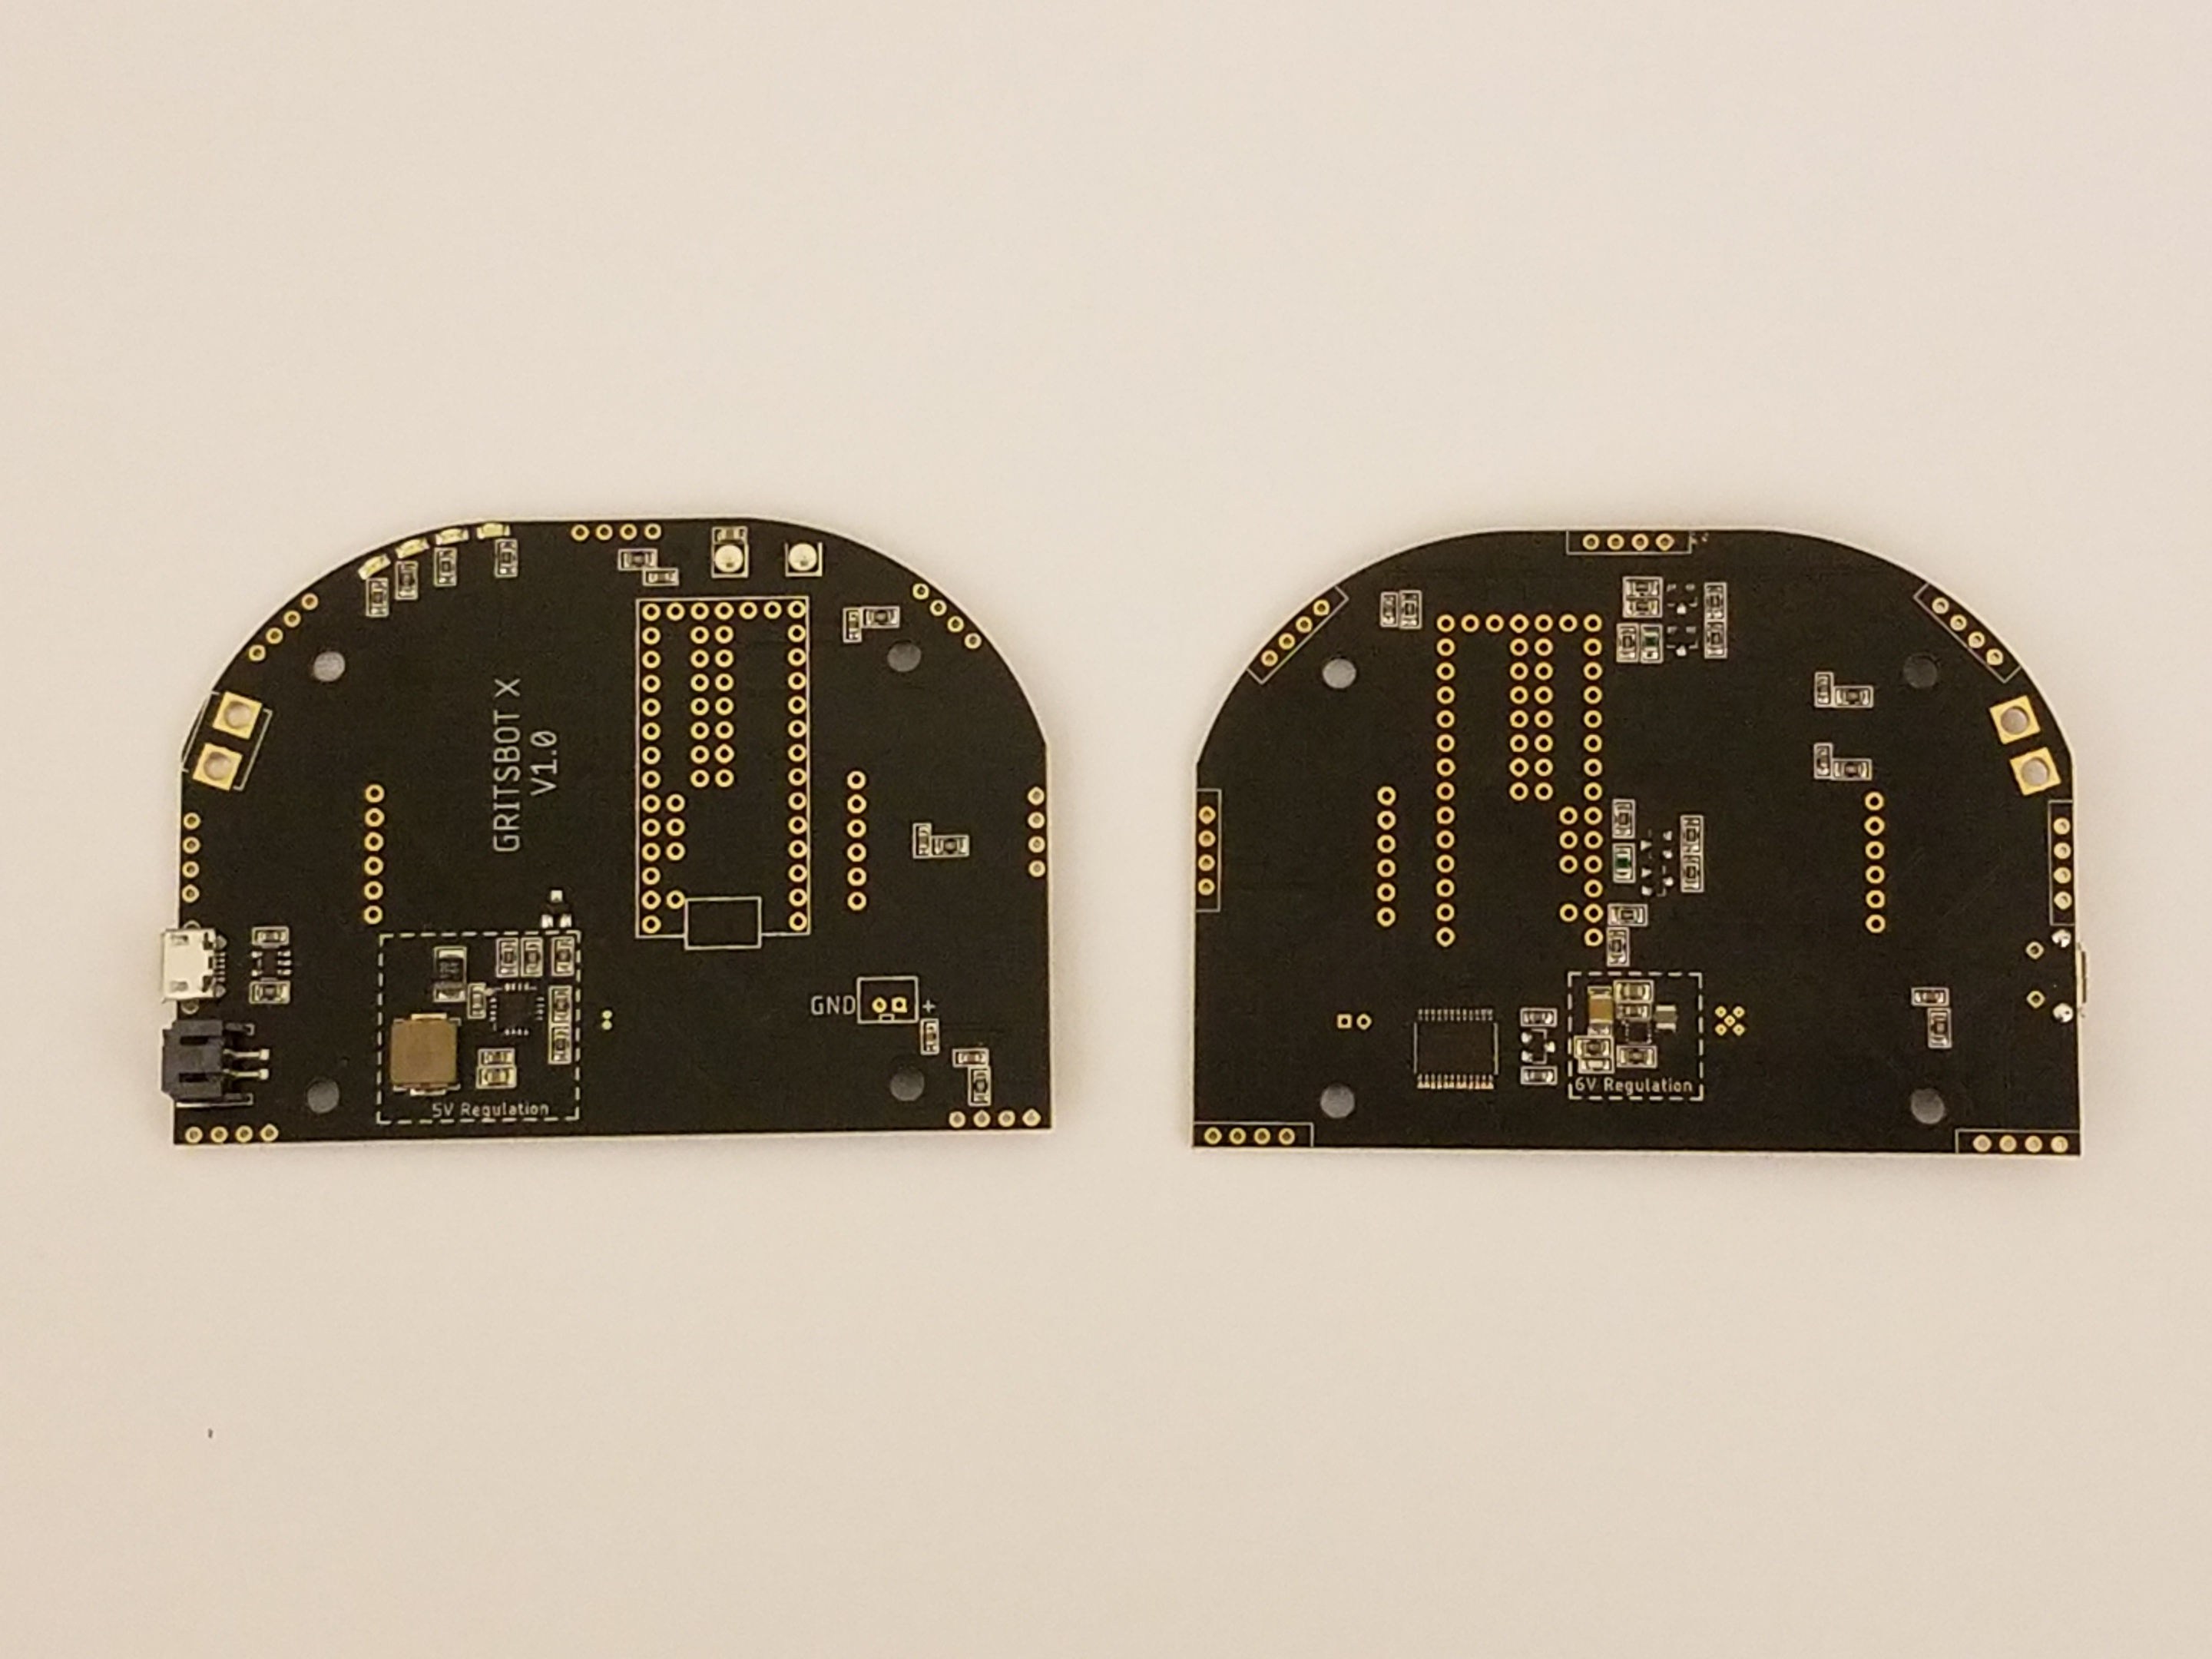
\includegraphics[width=0.65\columnwidth, keepaspectratio]{./figs/20181119_150313.jpg}
\caption{The main circuit board of the GRITSBot X after fabrication and partial assembly. This is the assumed starting point for PCB assembly.}
\label{fig:pcbPlain}
\end{figure}
%End PCB Picture straight from Circuithub
\vspace{1cm}
\noindent\textbf{\large{Assembly of Piggyback Boards}}\\

 A piggyback board is essentially a PCB that connects to another PCB. The GRITSBot X leverages two of these pre-made boards, the Teensy 3.2 microcontroller \cite{teensy} and the Pololu Carrier with Sharp GP2Y0A60SZLF Analog Distance Sensor \cite{pololuDistance}. The Teesny 3.2 is a microcontroller that handles the low level actuator control and sensor acquisition of the GRITSBot X.  The Pololu Sharp IR distance carrier enables the easy use of the GP2Y0A60SZLF range sensor.
 
 \subsection{Teensy 3.2}
 
 \subsubsection{Assembly Steps}
 
 \begin{enumerate}
 \item Gather the required materials (\cref{sec:teensyMaterials}).
 \item Solder the first set of male breakaway headers to the board leaving the left side unpopulated (\cref{sec:teensyFirstSolder}). 
 \item Mount and solder the surface mount header pins to the underside of the Teensy (\cref{sec:teensySecondSolder}).
 \item Finish soldering the header pins to the Teensy by populating the left side (\cref{sec:teensyFinalSolder}).
 \end{enumerate}
 
 %%% Teensy Materials Subsection
 \subsubsection{Required Materials}
 \label{sec:teensyMaterials}
 
 First, gather the required materials. The Teensy 3.2 microcontroller from PJRC, \cref{fig:teensyTB}, should come with the board and a $1 \times 36$ male breakaway header pin. If your Teensy did not come with male breakaway header pins, they are extremely inexpensive and can be purcased at a variety of locations.
 
 %Teensy 3.2 Picture.
\begin{figure}[h!]
\centering
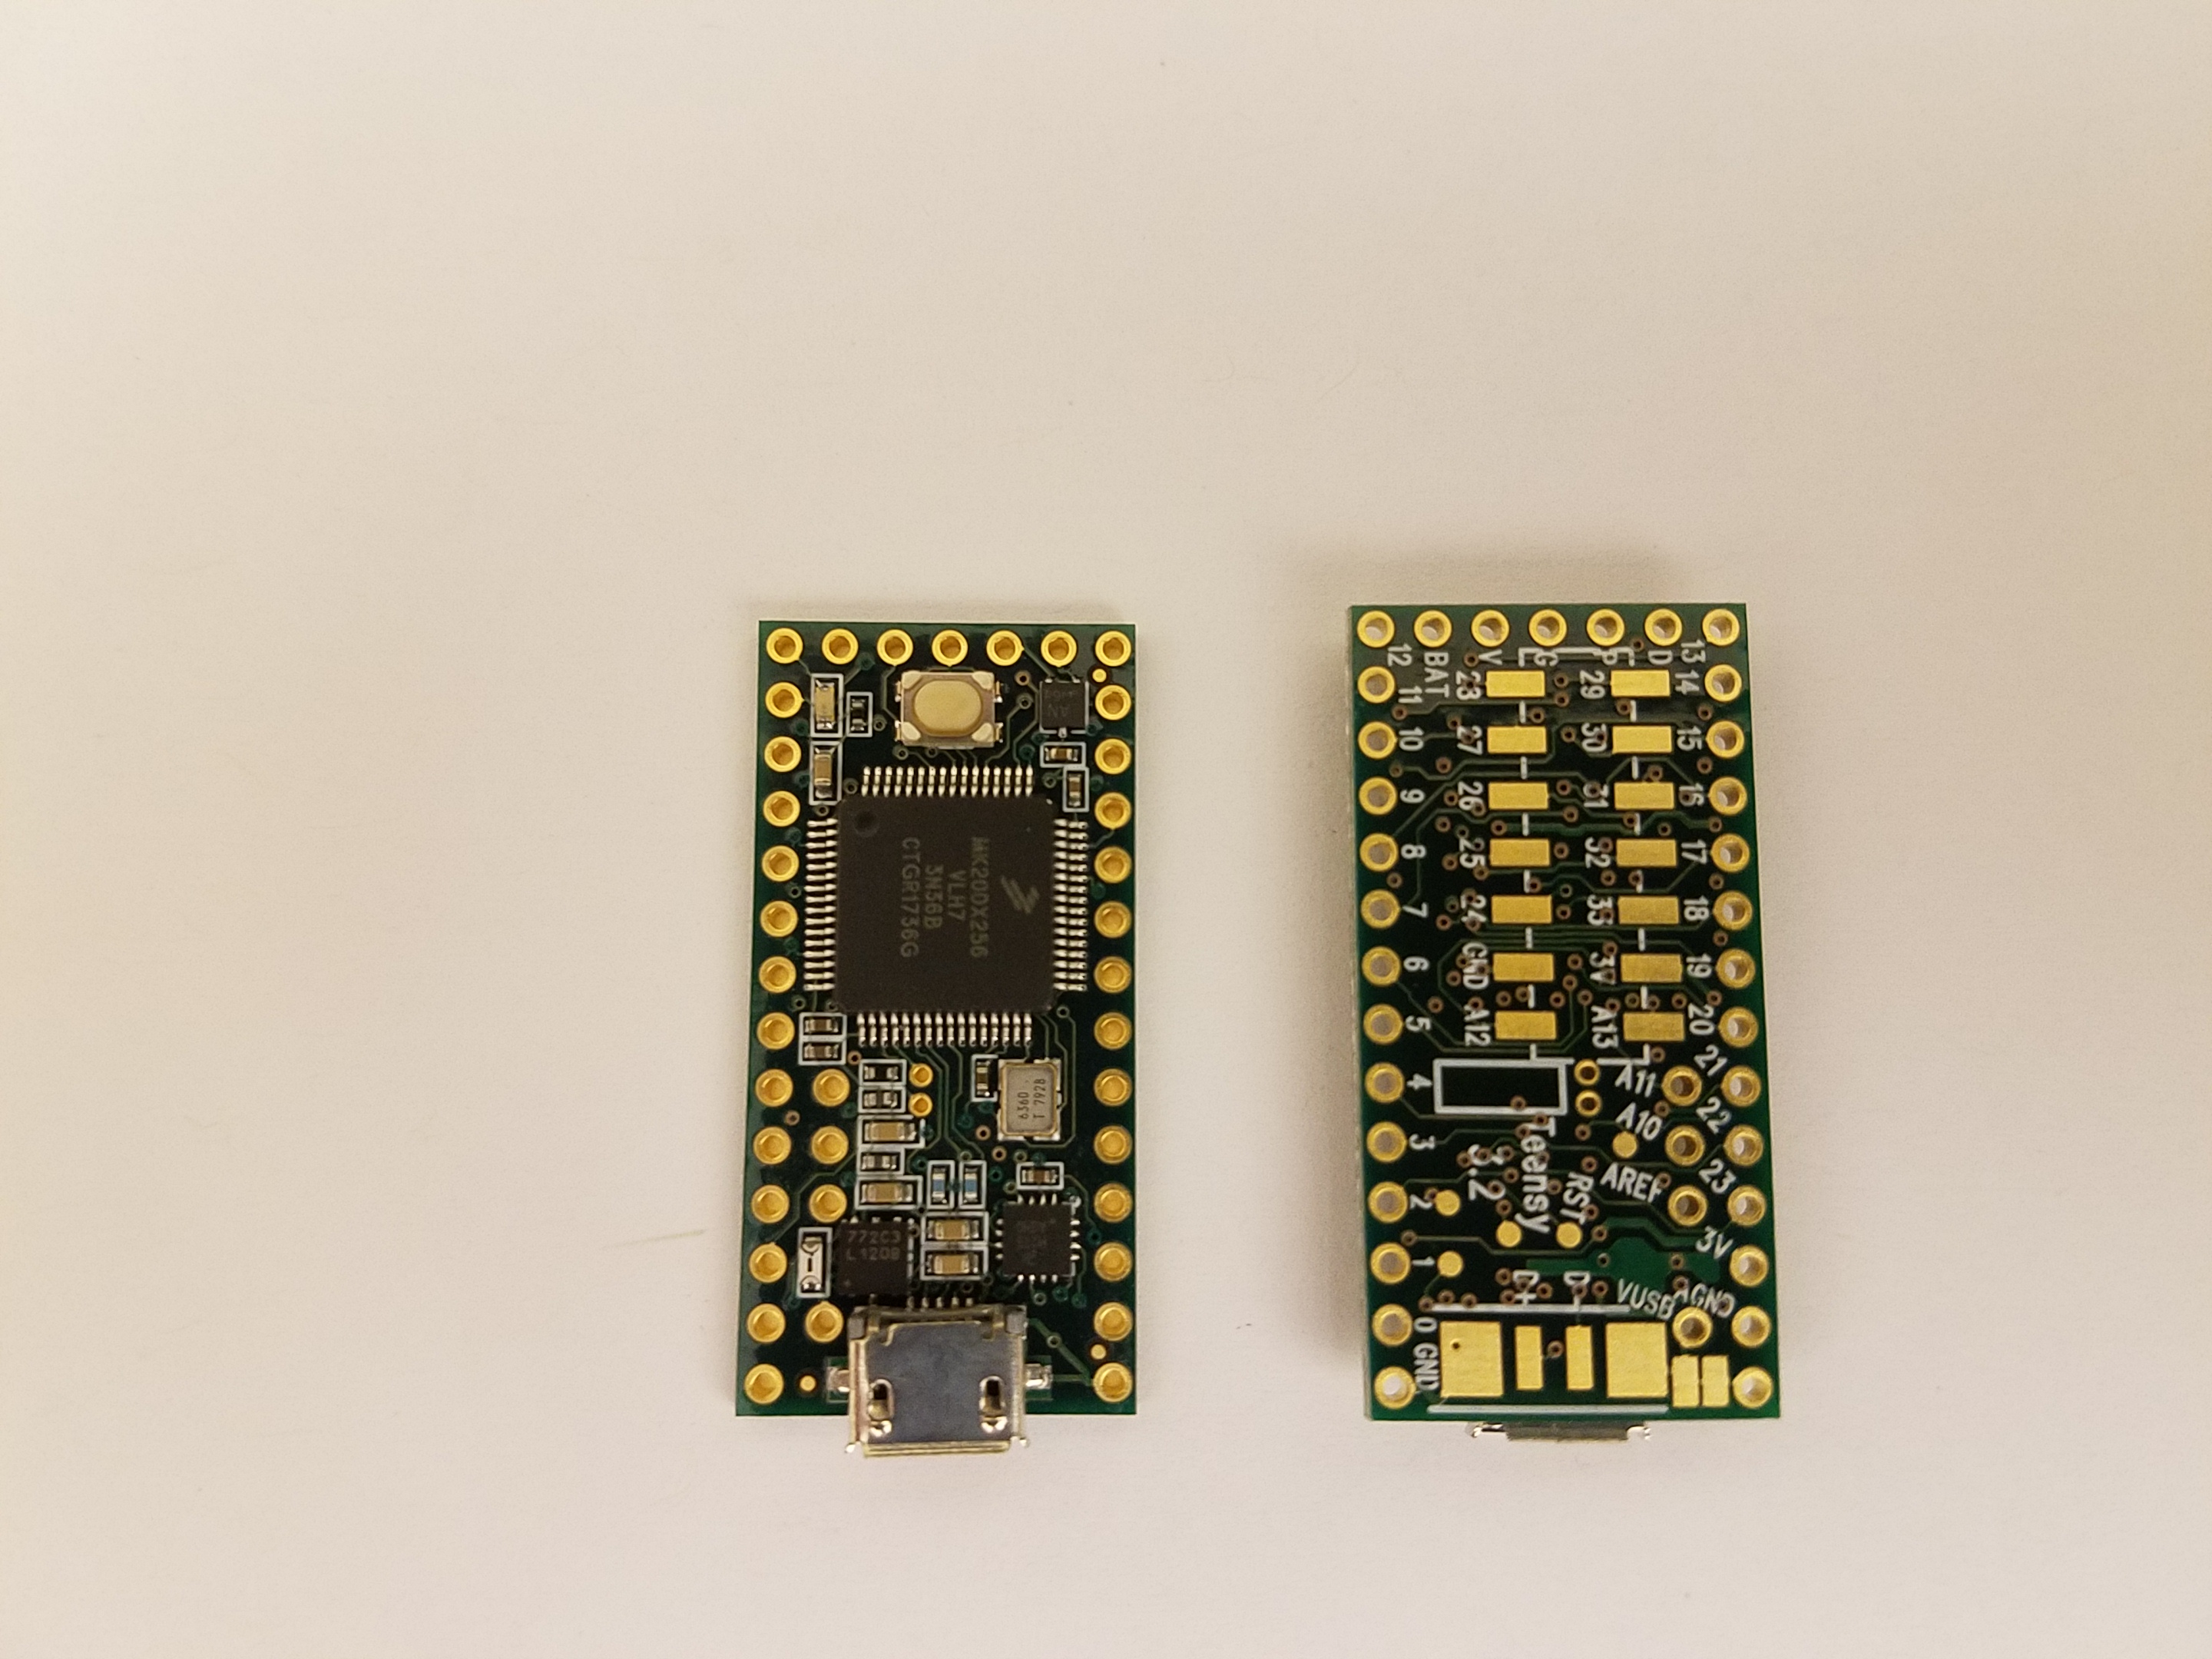
\includegraphics[trim={15cm 0 0 10cm},clip=true,width=0.65\columnwidth, keepaspectratio]{./figs/20181119_151744.jpg}
\caption{The Teensy 3.2 microcontroller top (\textbf{left}) and bottom (\textbf{right}) view.}
\label{fig:teensyTB}
\end{figure}
%End Teensy 3.2 Picture
 
 First, break the $1 \times 36$ breakaway header into smaller sections as described in \cref{tab:teensyBreakaway}. You may notice the number of male headers here totals 37 not the 36 provided with the board. You may either find a spare (recommended) or not populate the VUSB through hole.
 
  %Begin Teensy Part Table
 \begin{table}[h!]
 \centering
\begin{tabular}{ll}
\rowcolor[HTML]{C0C0C0} 
Number Required & Breakaway Dimension \\
2               & $1 \times  14$              \\
\rowcolor[HTML]{C0C0C0} 
1               & $1 \times 5$               \\
1               & $1 \times 3$               \\
\rowcolor[HTML]{C0C0C0} 
1               & $1 \times 1$              
\end{tabular}
\caption{The dimensions of the male breakaway headers needed to assemble the Teensy 3.2 microcontroller. \label{tab:teensyBreakaway}}
\end{table}
 %End Teensy Part Table

We also require the surface mount pins available on the underside of the Teensy 3.2 as seen in the right side of \cref{fig:teensyTB}. This requires a 14 position surface mount header and broken perforated board pictured in the bottom of \cref{fig:teensyParts}. Now that we have all the parts we can begin soldering this board together.

 %Teensy Parts Picture
\begin{figure}[h!]
\centering
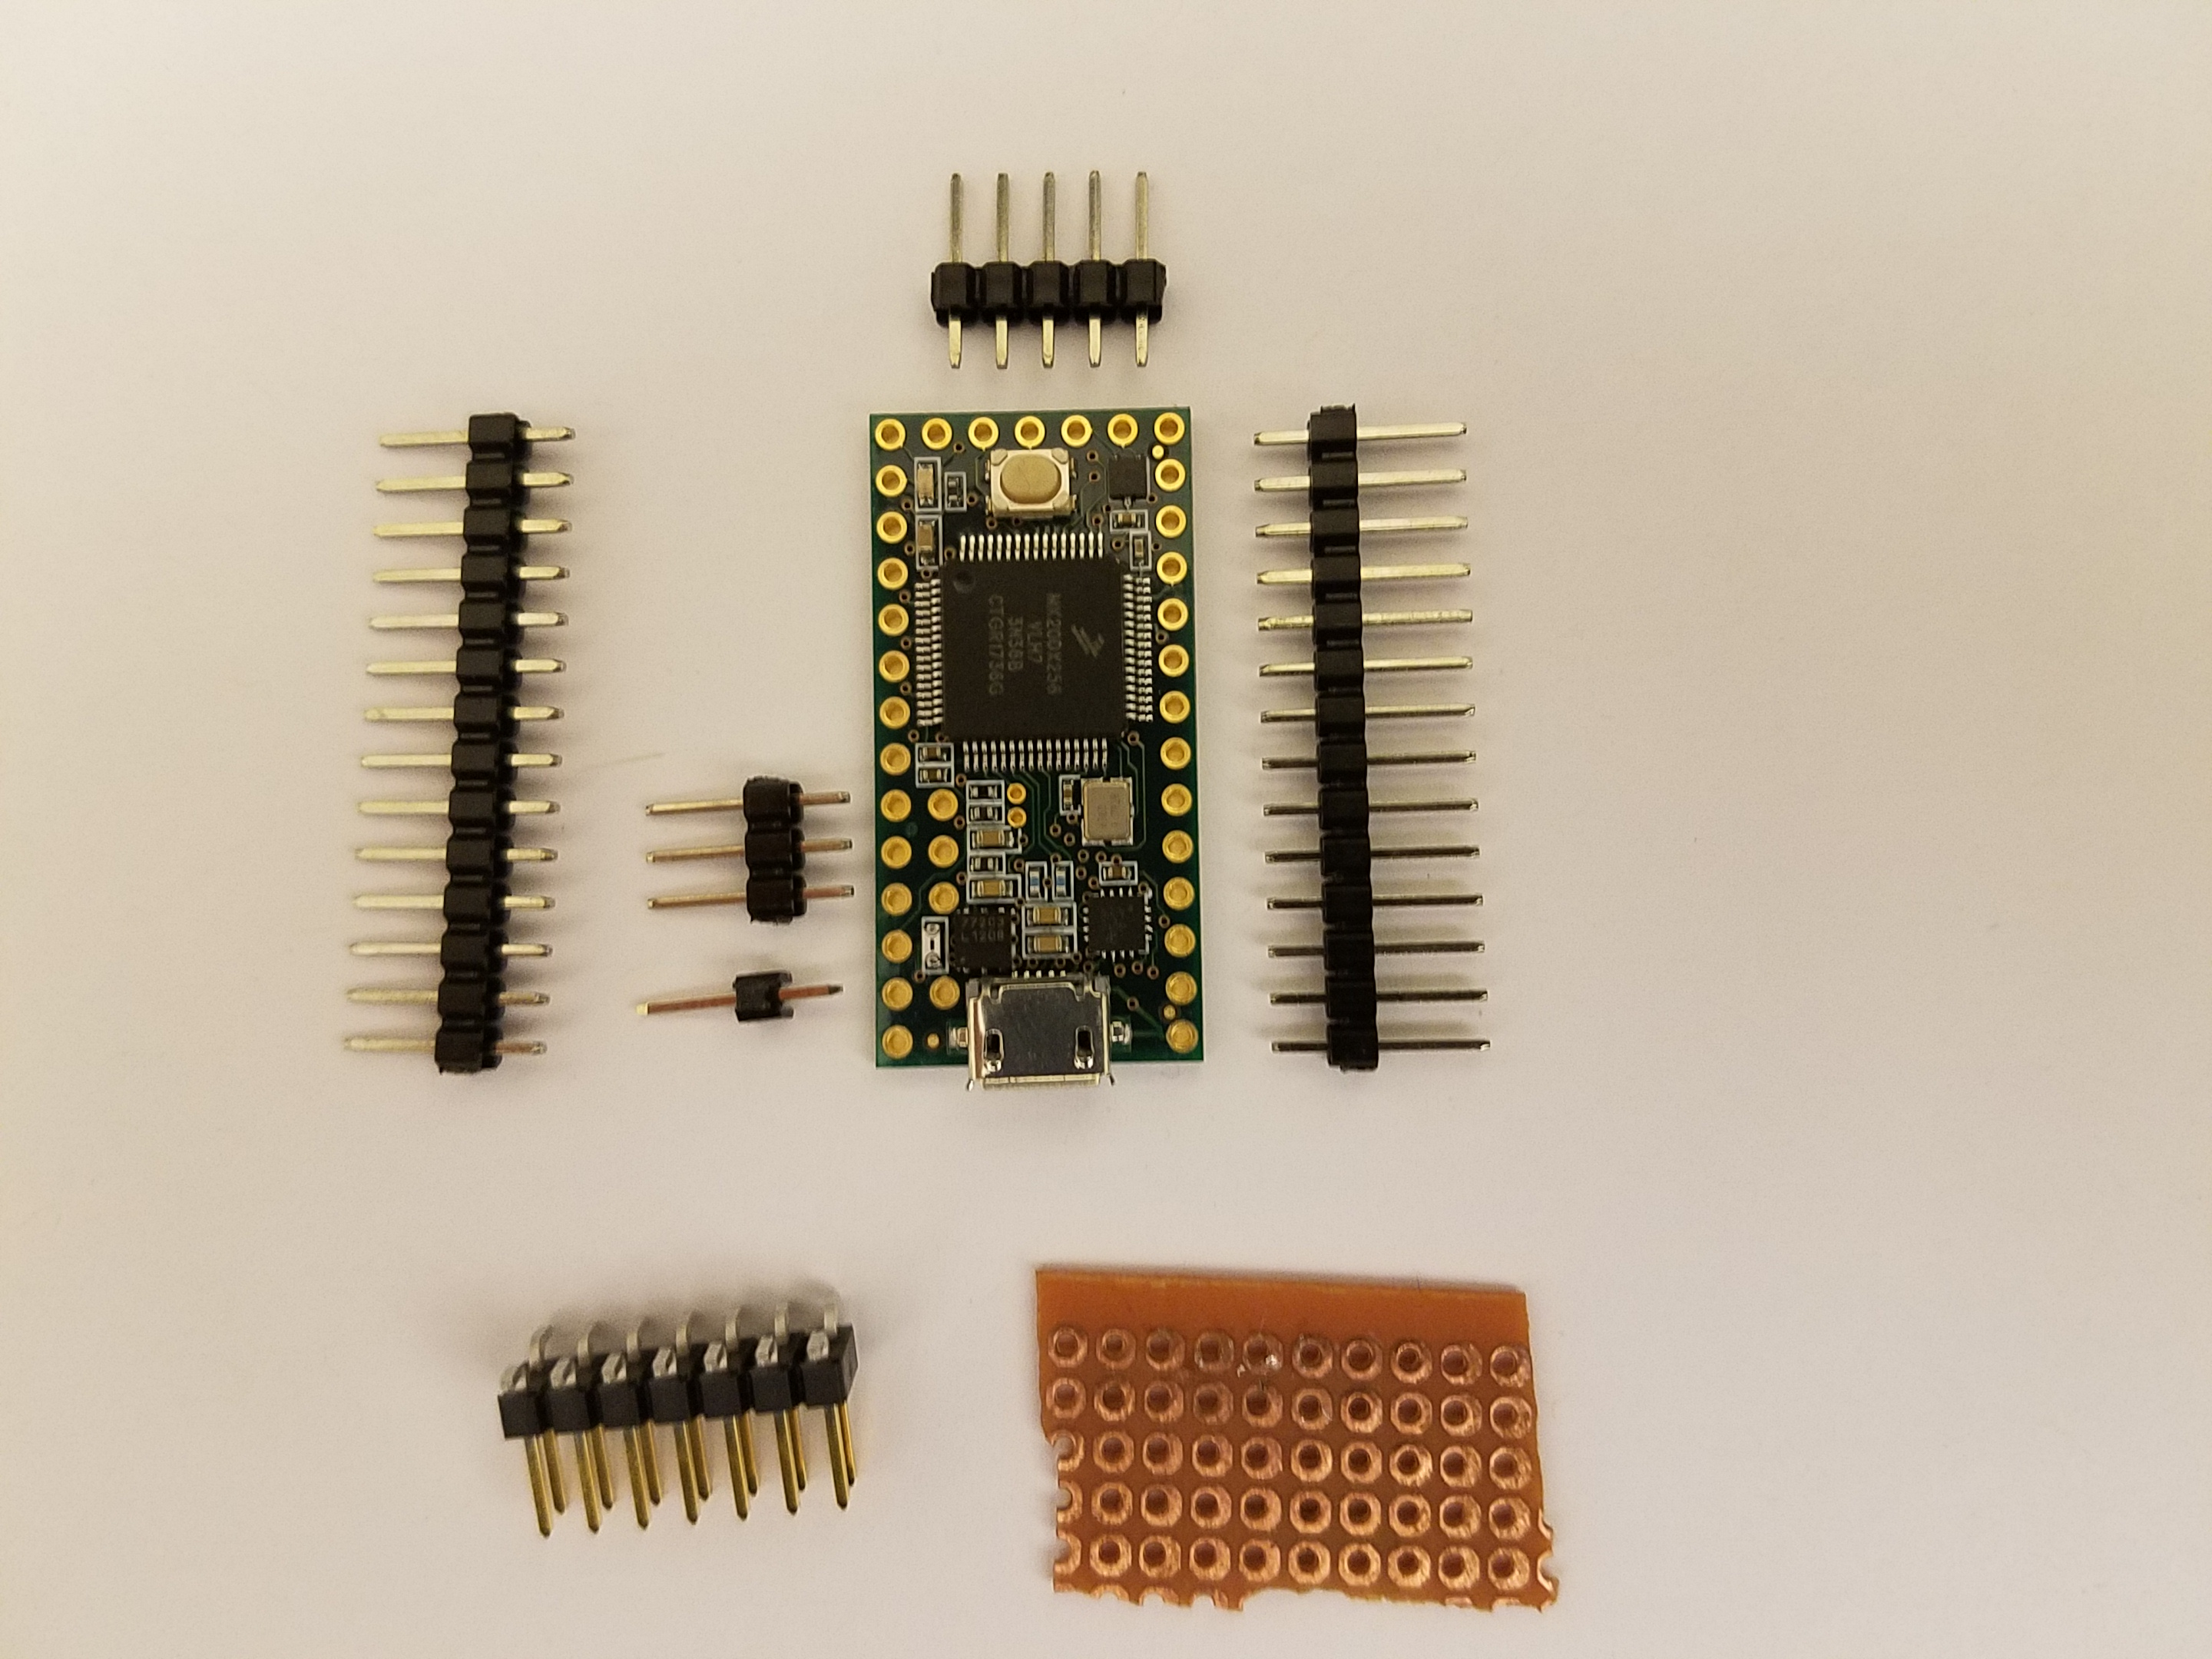
\includegraphics[width=0.65\columnwidth, keepaspectratio]{./figs/20181119_160924.jpg}
\caption{The parts needed to solder header pins to the Teensy 3.2 microcontroller.}
\label{fig:teensyParts}
\end{figure}
%End Teensy Parts Picture

%%%First Solder Pass Subsection (Male Headers)
\subsubsection{Creating Perpendicular Solder Points and the First Solder Pass}
\label{sec:teensyFirstSolder}

Using the main PCB as a guide, slide all the male breakaway headers (excluding the surface mount ones) into the PCB (\cref{fig:teensyMaleHeader}) and place the Teensy 3.2 on top (\cref{fig:teensyMountedMaleHeader}) as shown in \cref{fig:teensyFirstPass}. \textbf{\textcolor{red}{Before soldering}}, observe the proximity of the header pads to the main processor chip (big black square) connections. When soldering be very carful not to accidentally solder or bridge these connections. It is best to keep the iron and solder being applied on the outside perimeter of the board. At this point solder all of the header pins on the Teensy {\textcolor{red}{\textbf{except}}} the left side headers as seen in \cref{fig:teensyFirstSolder}. It is extremely important that the left side header pins be left unpopulated for now so there is enough room for the soldering iron to attach the surface mount headers in the next step.

 %Male headers in PCB picture
\begin{figure}[h!]
\centering
\subfloat[\label{fig:teensyMaleHeader}]{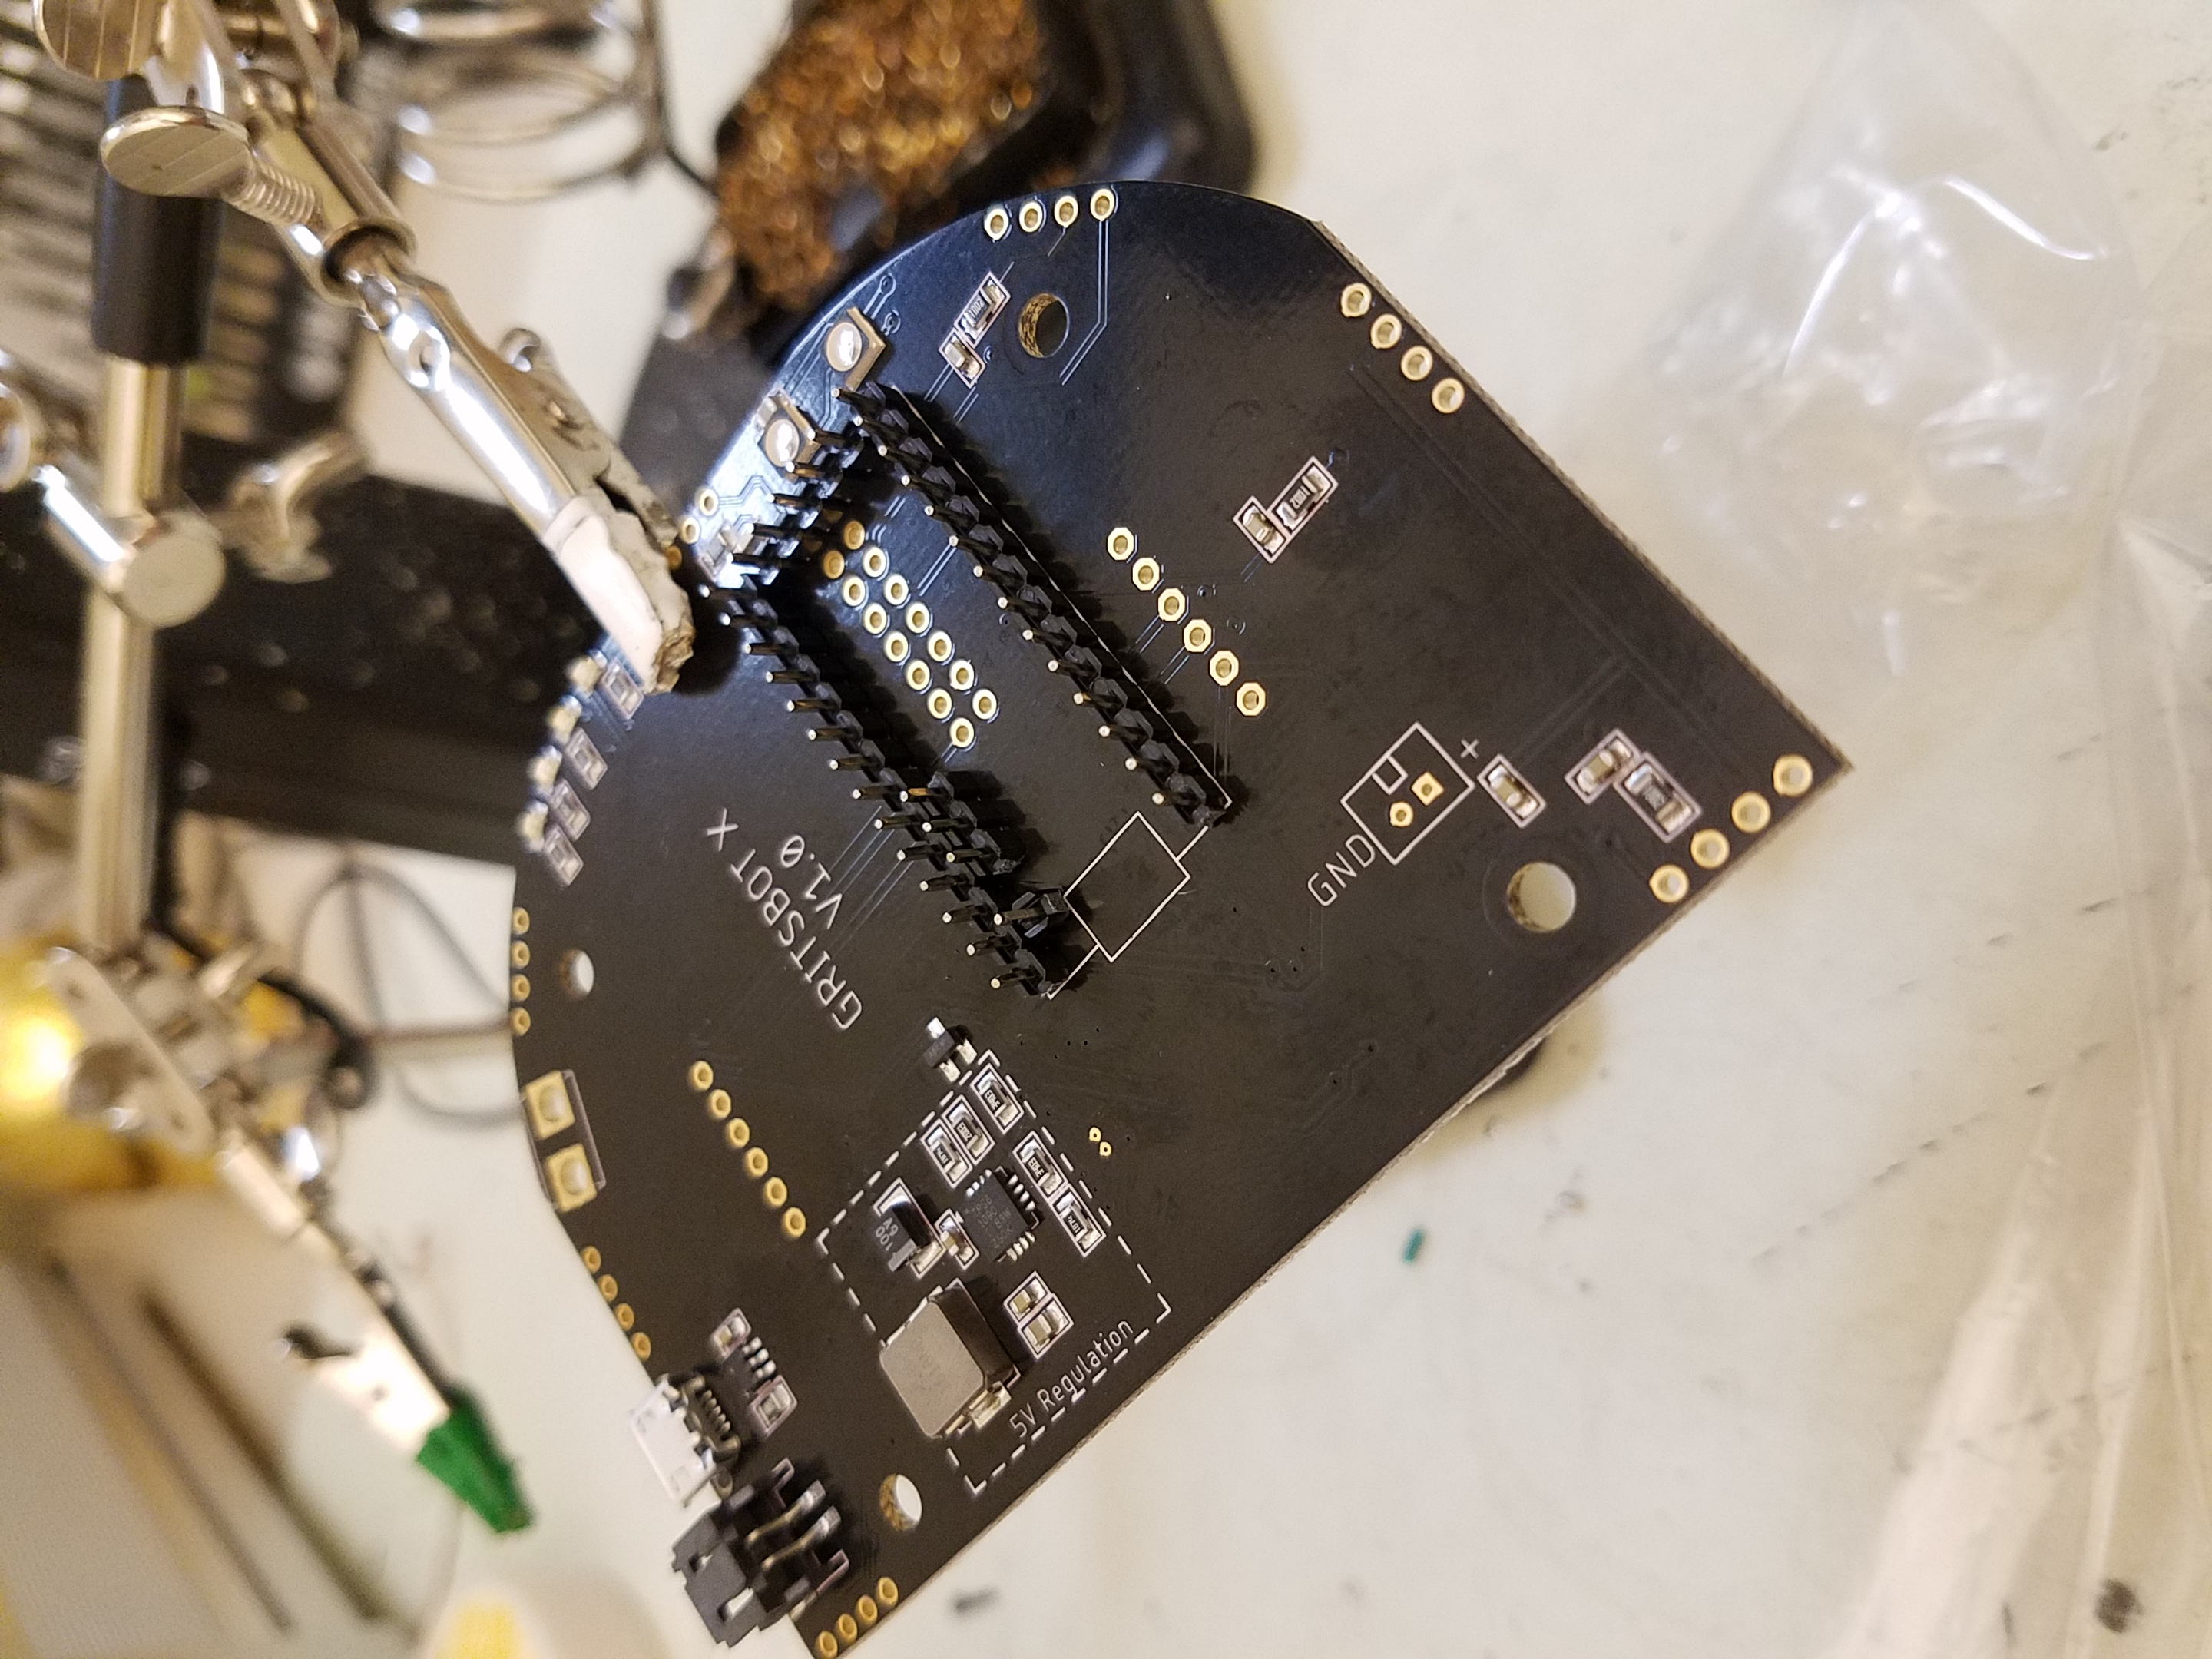
\includegraphics[width=0.45\columnwidth, keepaspectratio]{./figs/20180911_105051.jpg}}
\hfill
\subfloat[\label{fig:teensyMountedMaleHeader}]{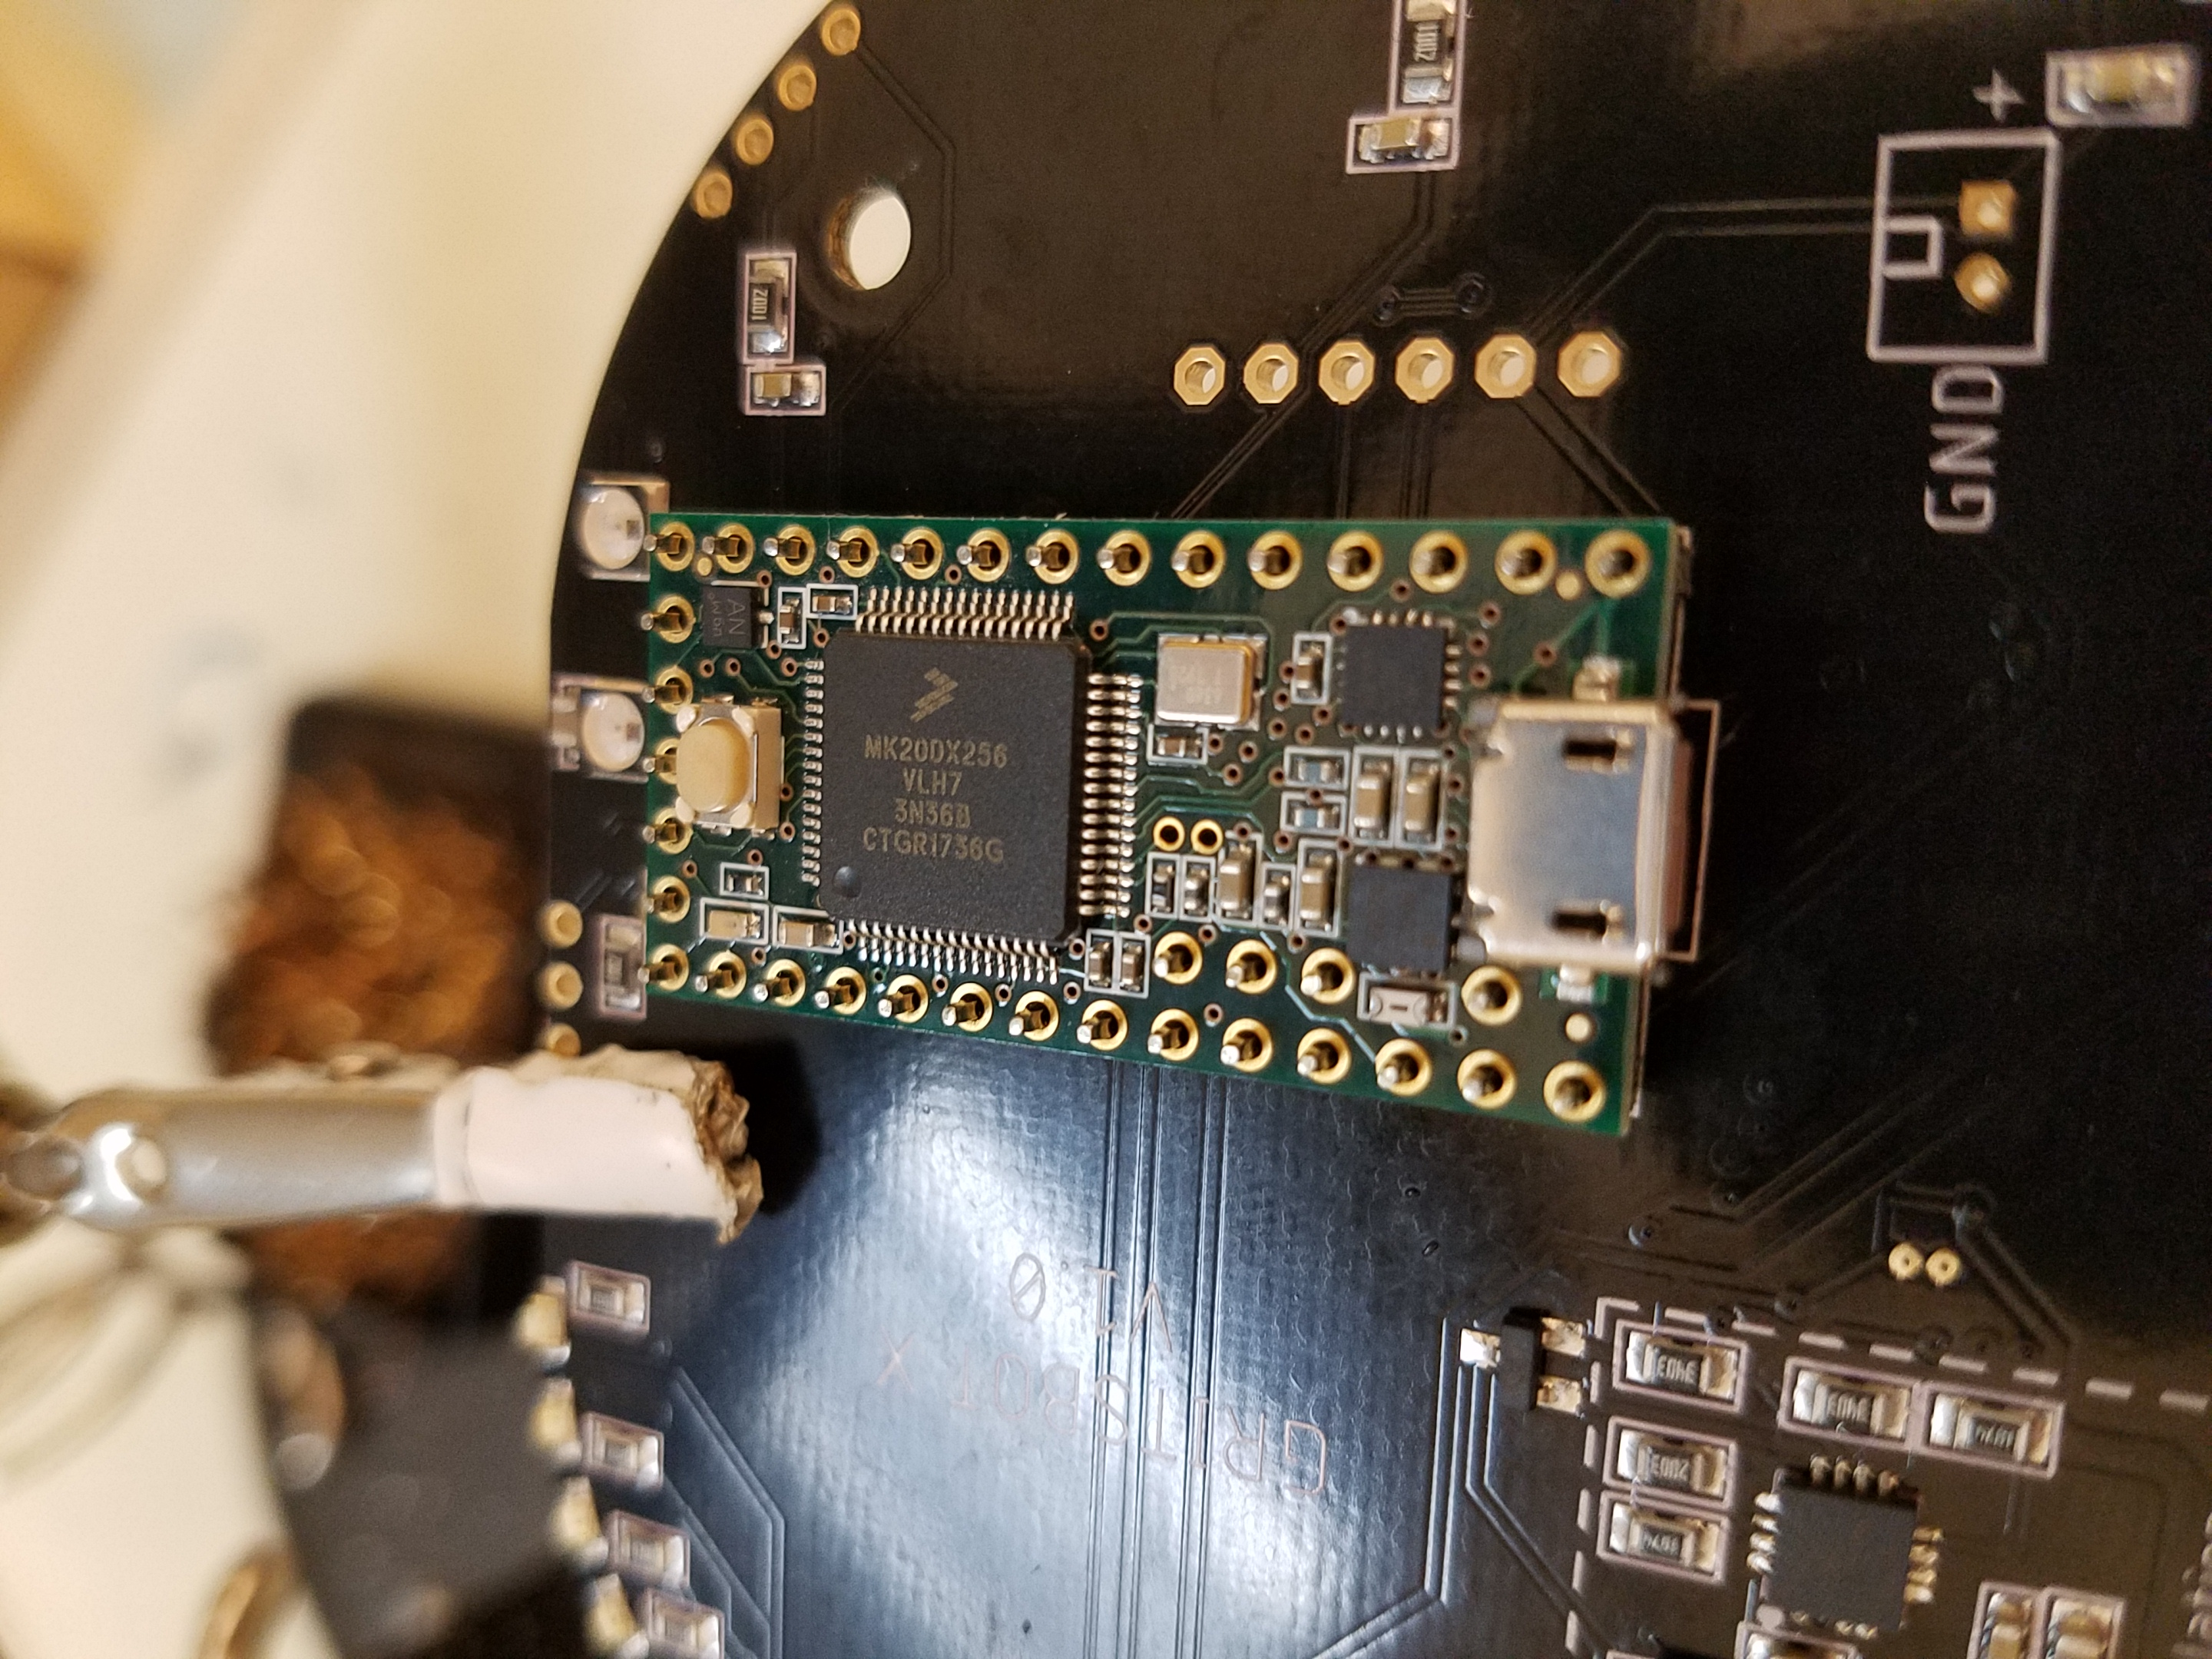
\includegraphics[width=0.45\columnwidth, keepaspectratio]{./figs/20180911_105154.jpg}}\\
\subfloat[\label{fig:teensyFirstSolder}]{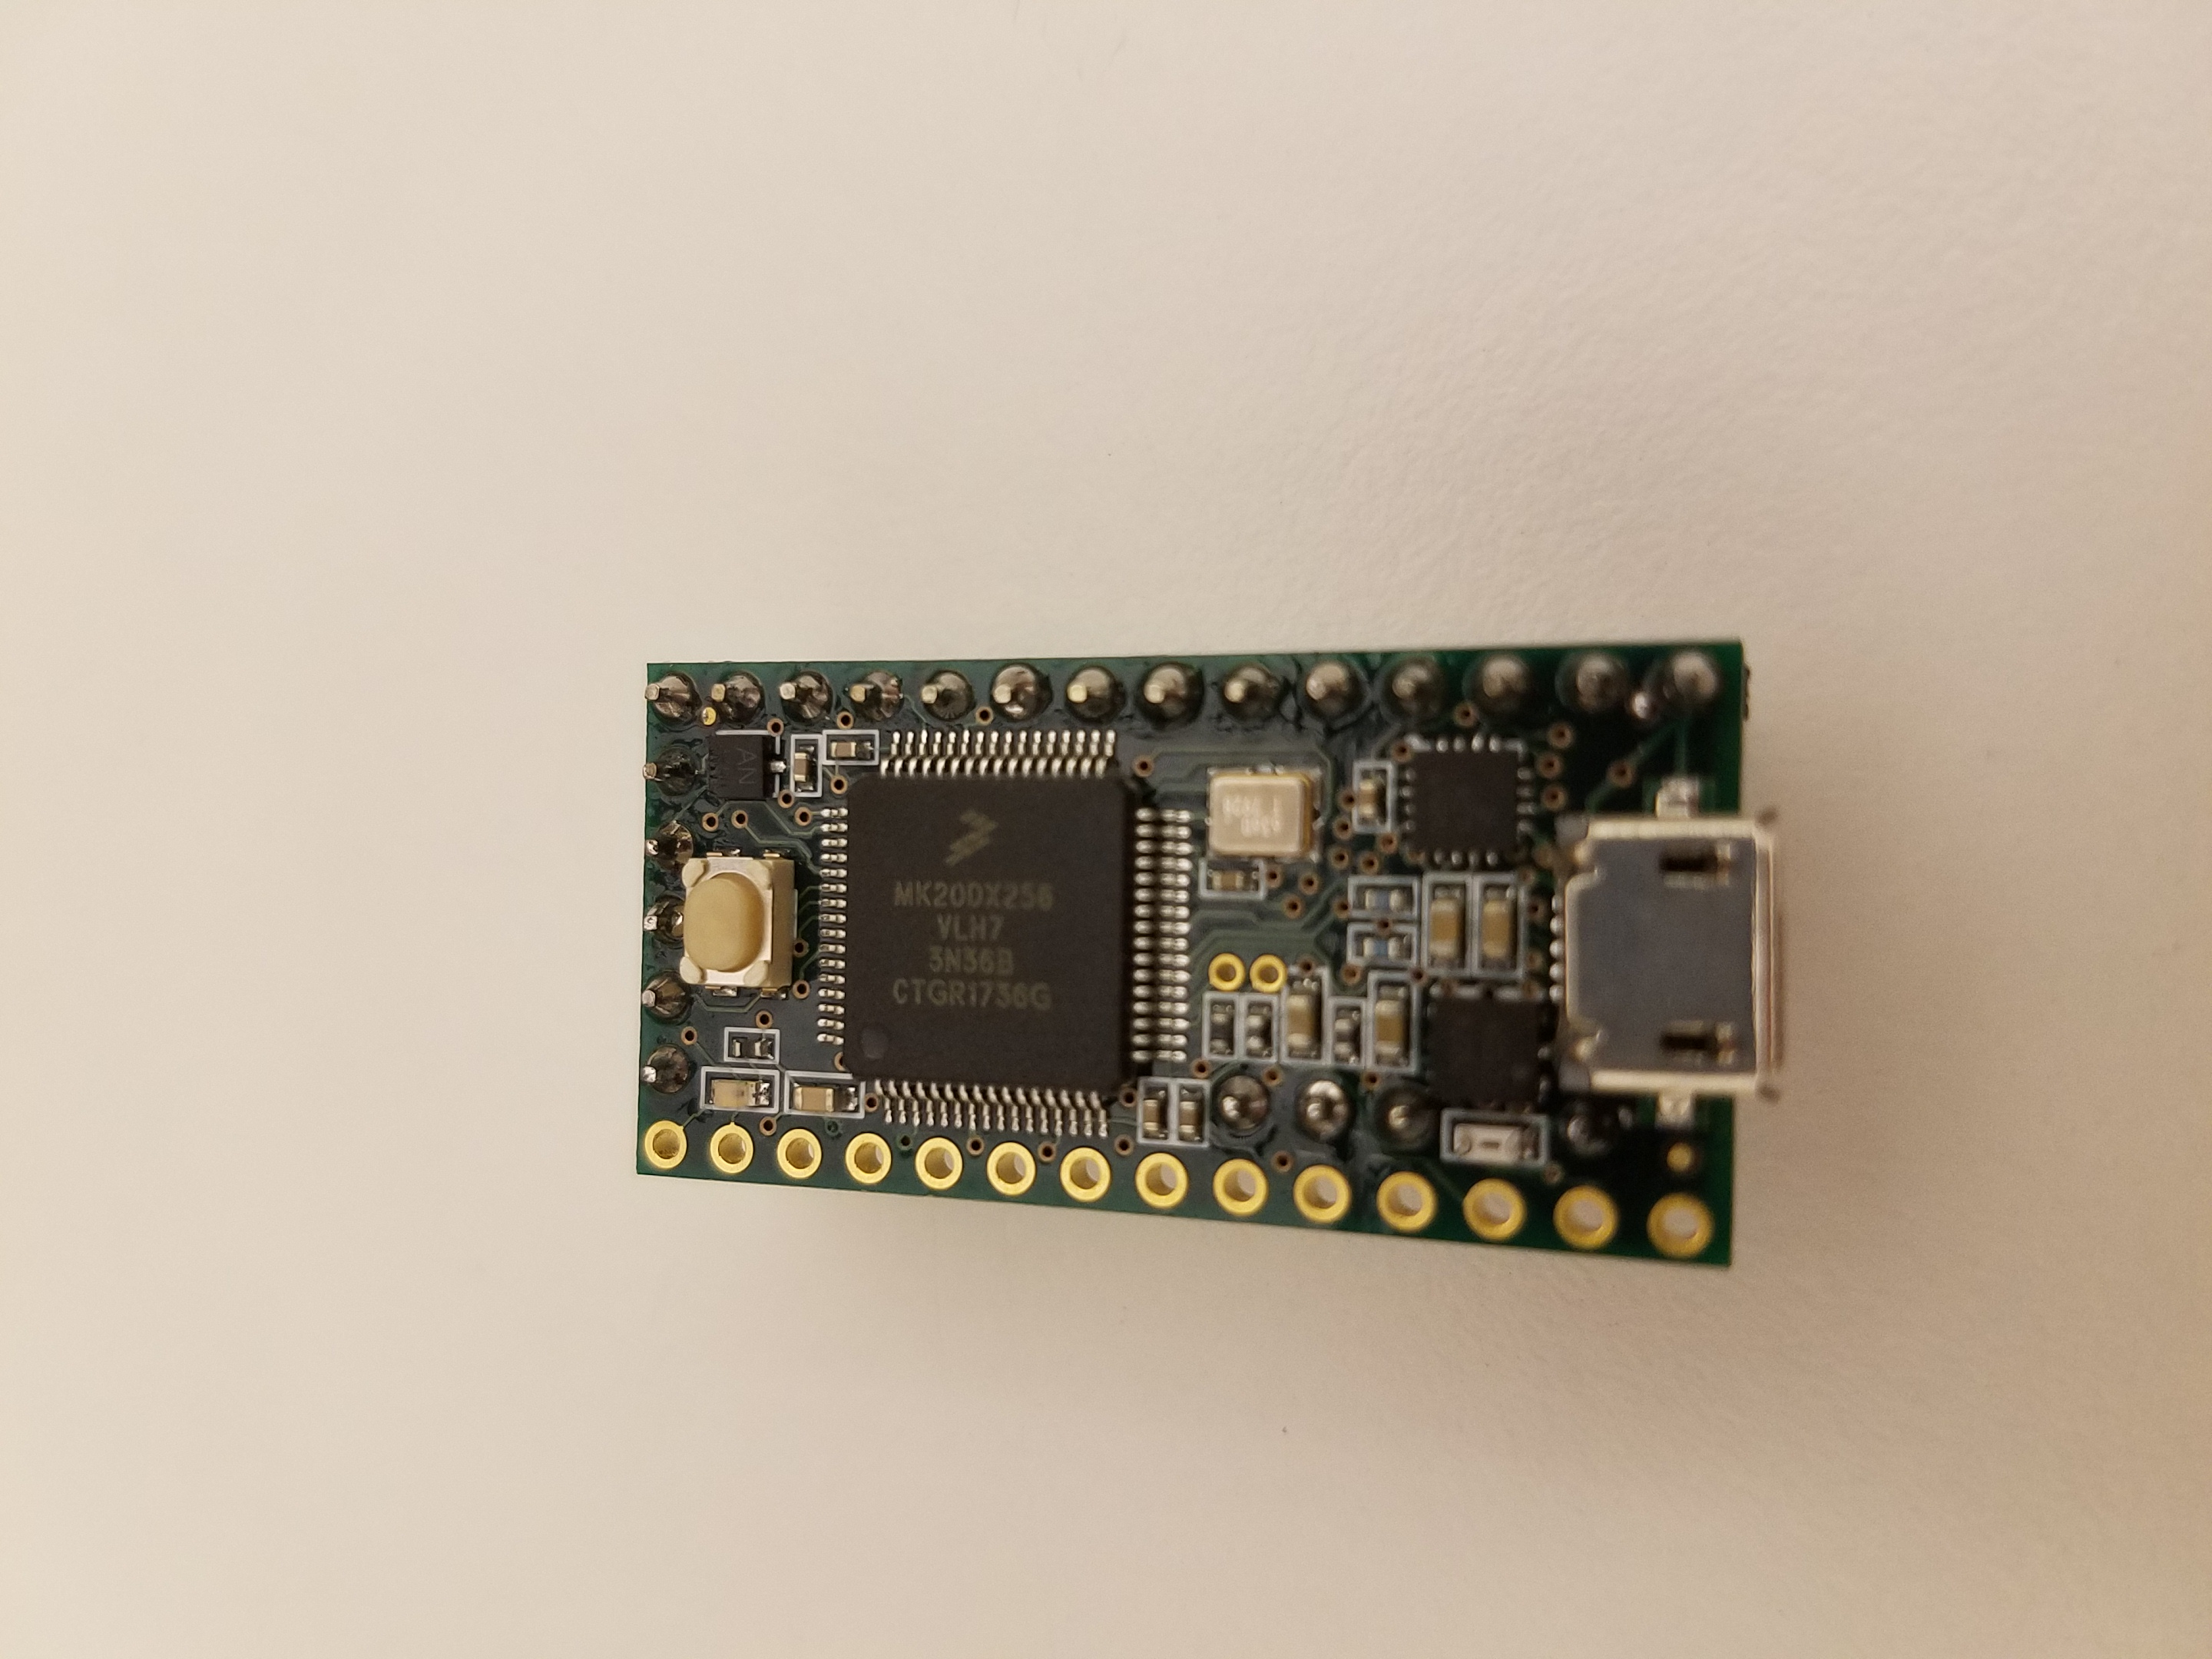
\includegraphics[width=0.45\columnwidth, keepaspectratio]{./figs/20180911_105434.jpg}}
\caption{Creating perpendicular solder points for the Teensy 3.2 using the GRITSBot X main PCB.}
\label{fig:teensyFirstPass}
\end{figure}
%End Male headers in PCB picture

%%%Second Solder Pass Subsection (Surface Mount)
\subsubsection{Soldering the Surface Mount Headers}
\label{sec:teensySecondSolder}

Now that the majority of the male headers have been soldered in place, we must now attach the surface mount headers. A major challenge here is mounting them so they align with the rest of the headers or the Teensy will not be able to fit into the main PCB of the GRITSBot X. To do this we will use the broken piece of perforated board, the 14 position surface mount header pins, and the Teensy that has been soldered so far (seen in \cref{fig:teensyMaterialsSecondSolder}).

 %Teensy Materials Surface Mount Picture
\begin{figure}[h!]
\centering
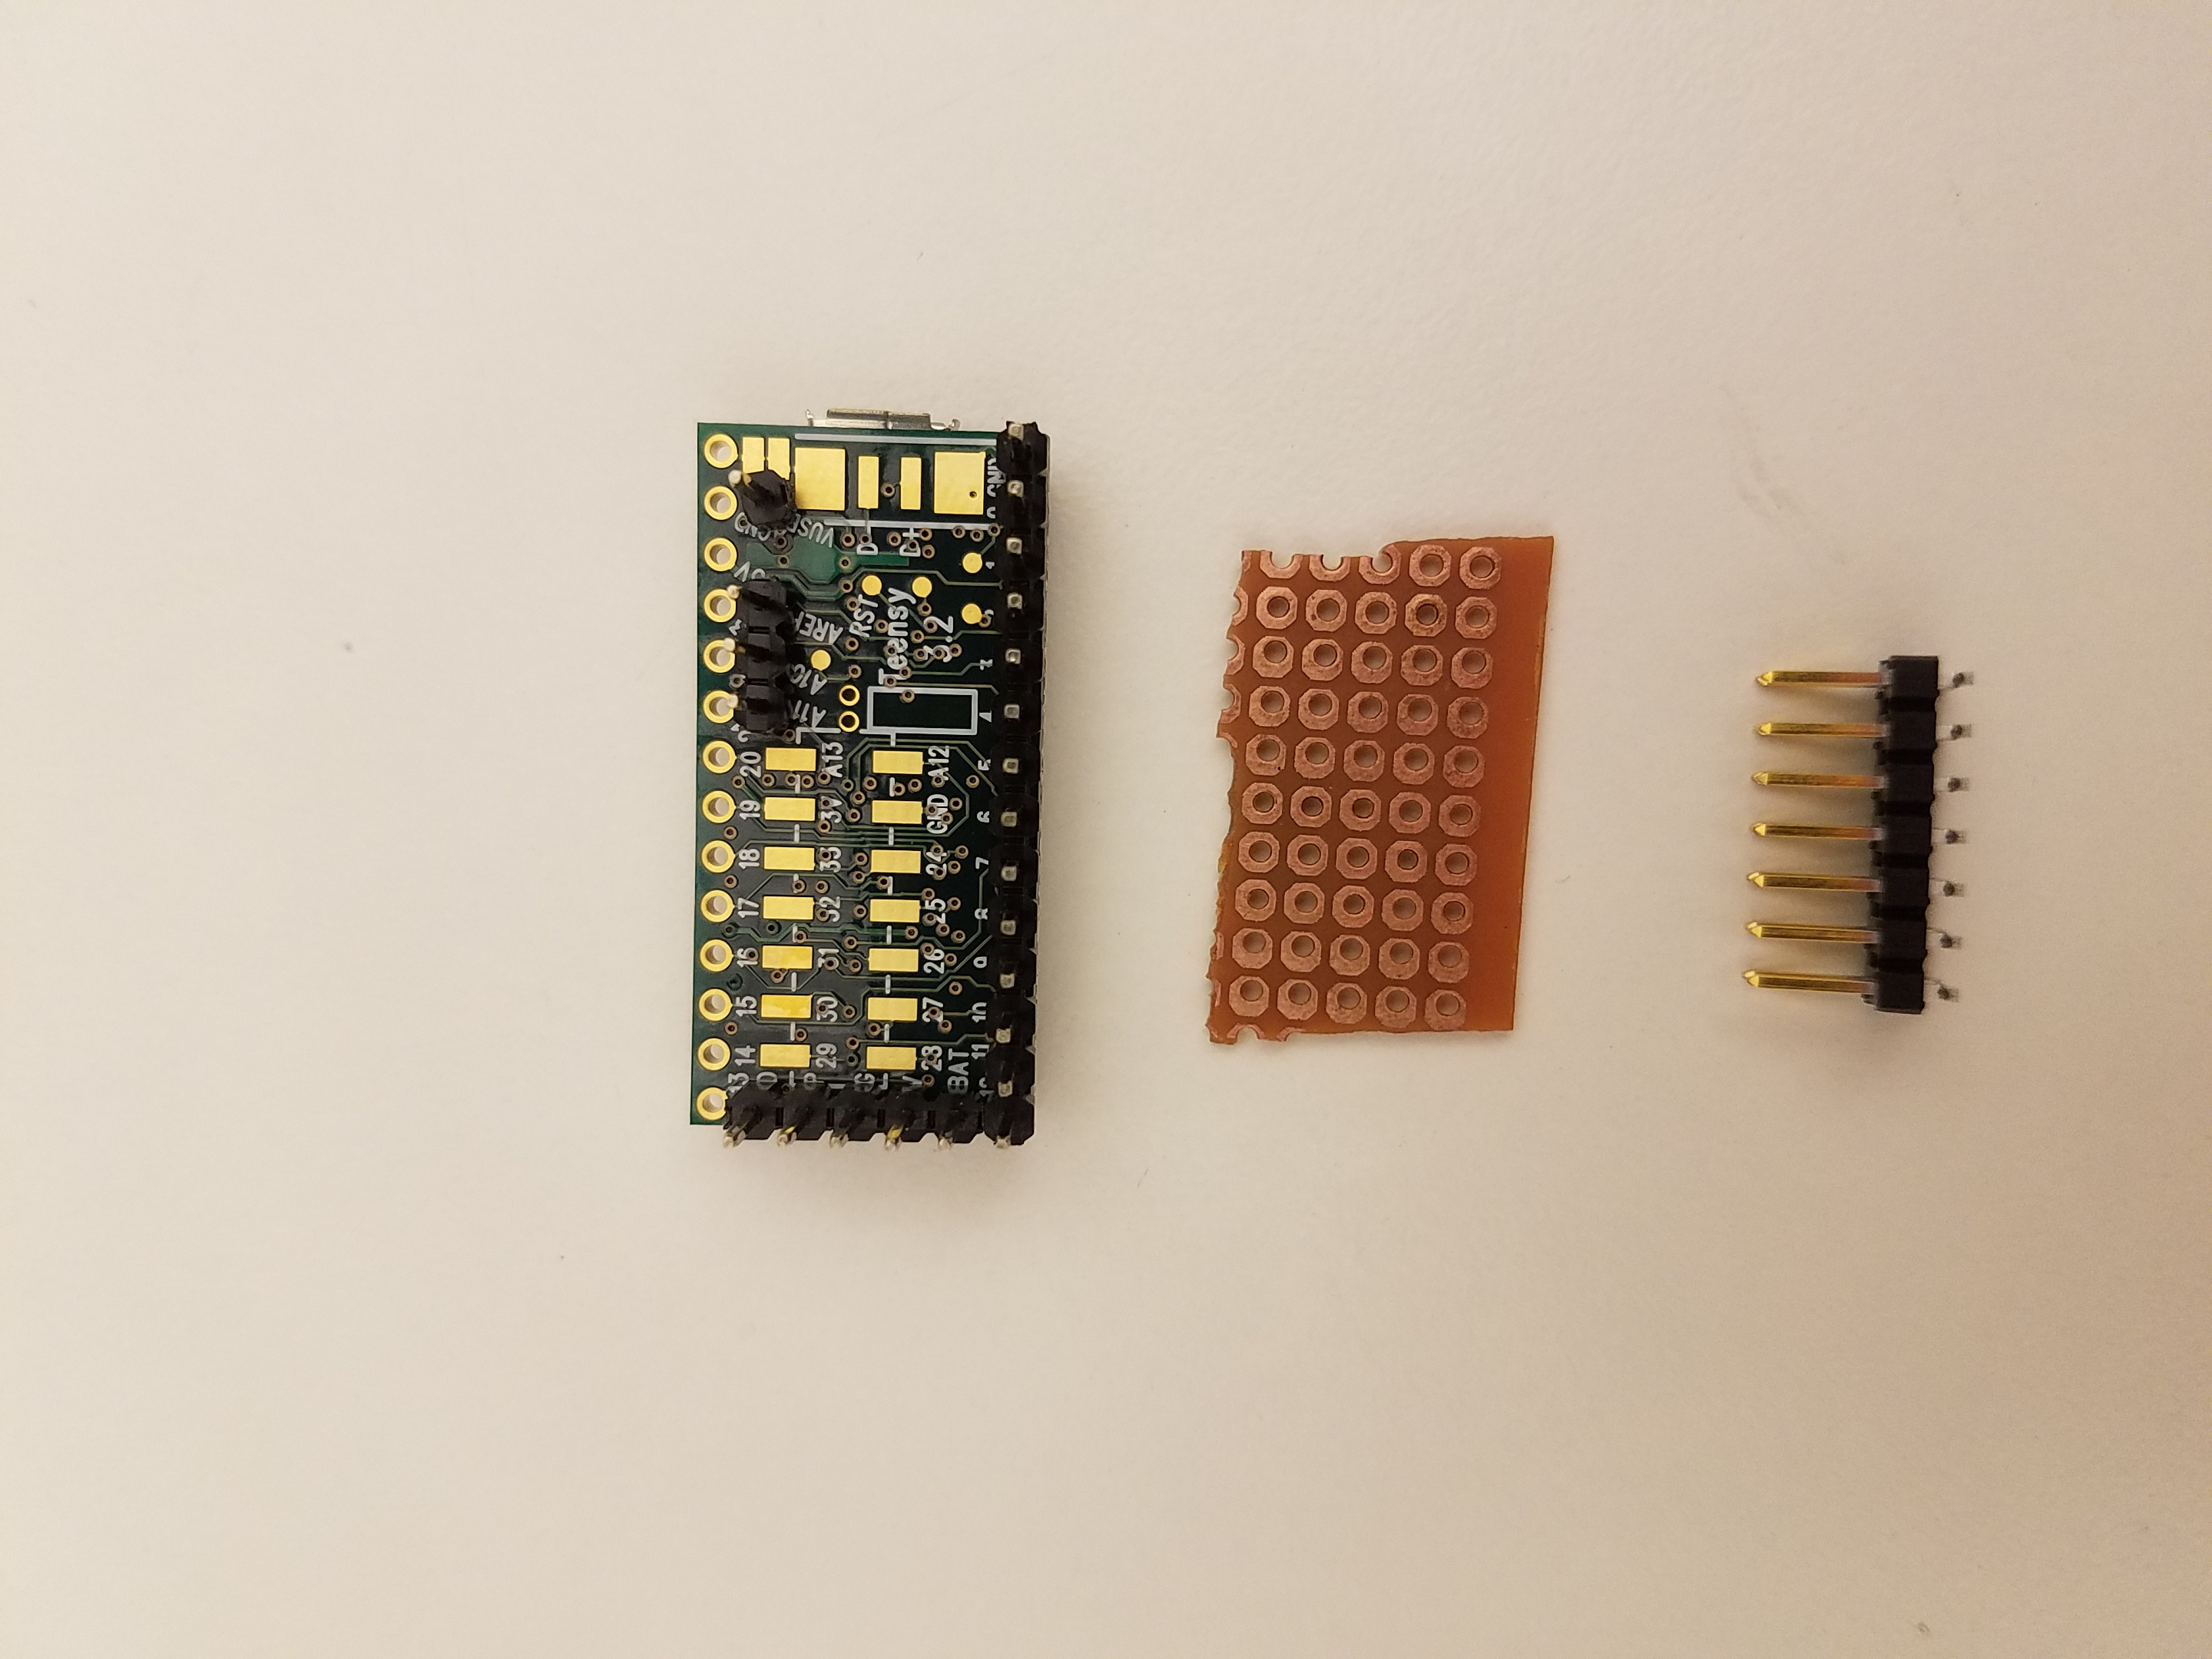
\includegraphics[trim={15cm 0 0 0},clip=true,width=0.65\columnwidth, keepaspectratio,angle=180]{./figs/20180911_105530.jpg}
\caption{The 14 position surface mount header, perforated board, and Teensy required to make the underside pins of the Teensy accessible.}
\label{fig:teensyMaterialsSecondSolder}
\end{figure}
%End Teensy Materials Surface Mount Picture  

Insert the surface mount header pins into the broken perforated board leaving at least 6 pins exposed as seen in \cref{fig:surfaceHeaderPerf}. Note, in this picture 8 pins are left exposed. Inset the Teensy into the same perforated board such that the surface pads of the Teensy are aligned with the surface mount header pins as seen in \cref{fig:surfaceHeaderPerfTeensy}. Make sure the surface mount headers are pressed into the Teensy pads and solder the first few pad, header connections into place with the perforated board keeping them aligned. After the solder cools, remove the perforated board and solder the rest of the connections. Upon completion your board should resemble that in \cref{fig:surfaceHeaderTeensy}.

 %Male headers in PCB picture
\begin{figure}[h!]
\centering
\subfloat[\label{fig:surfaceHeaderPerf}]{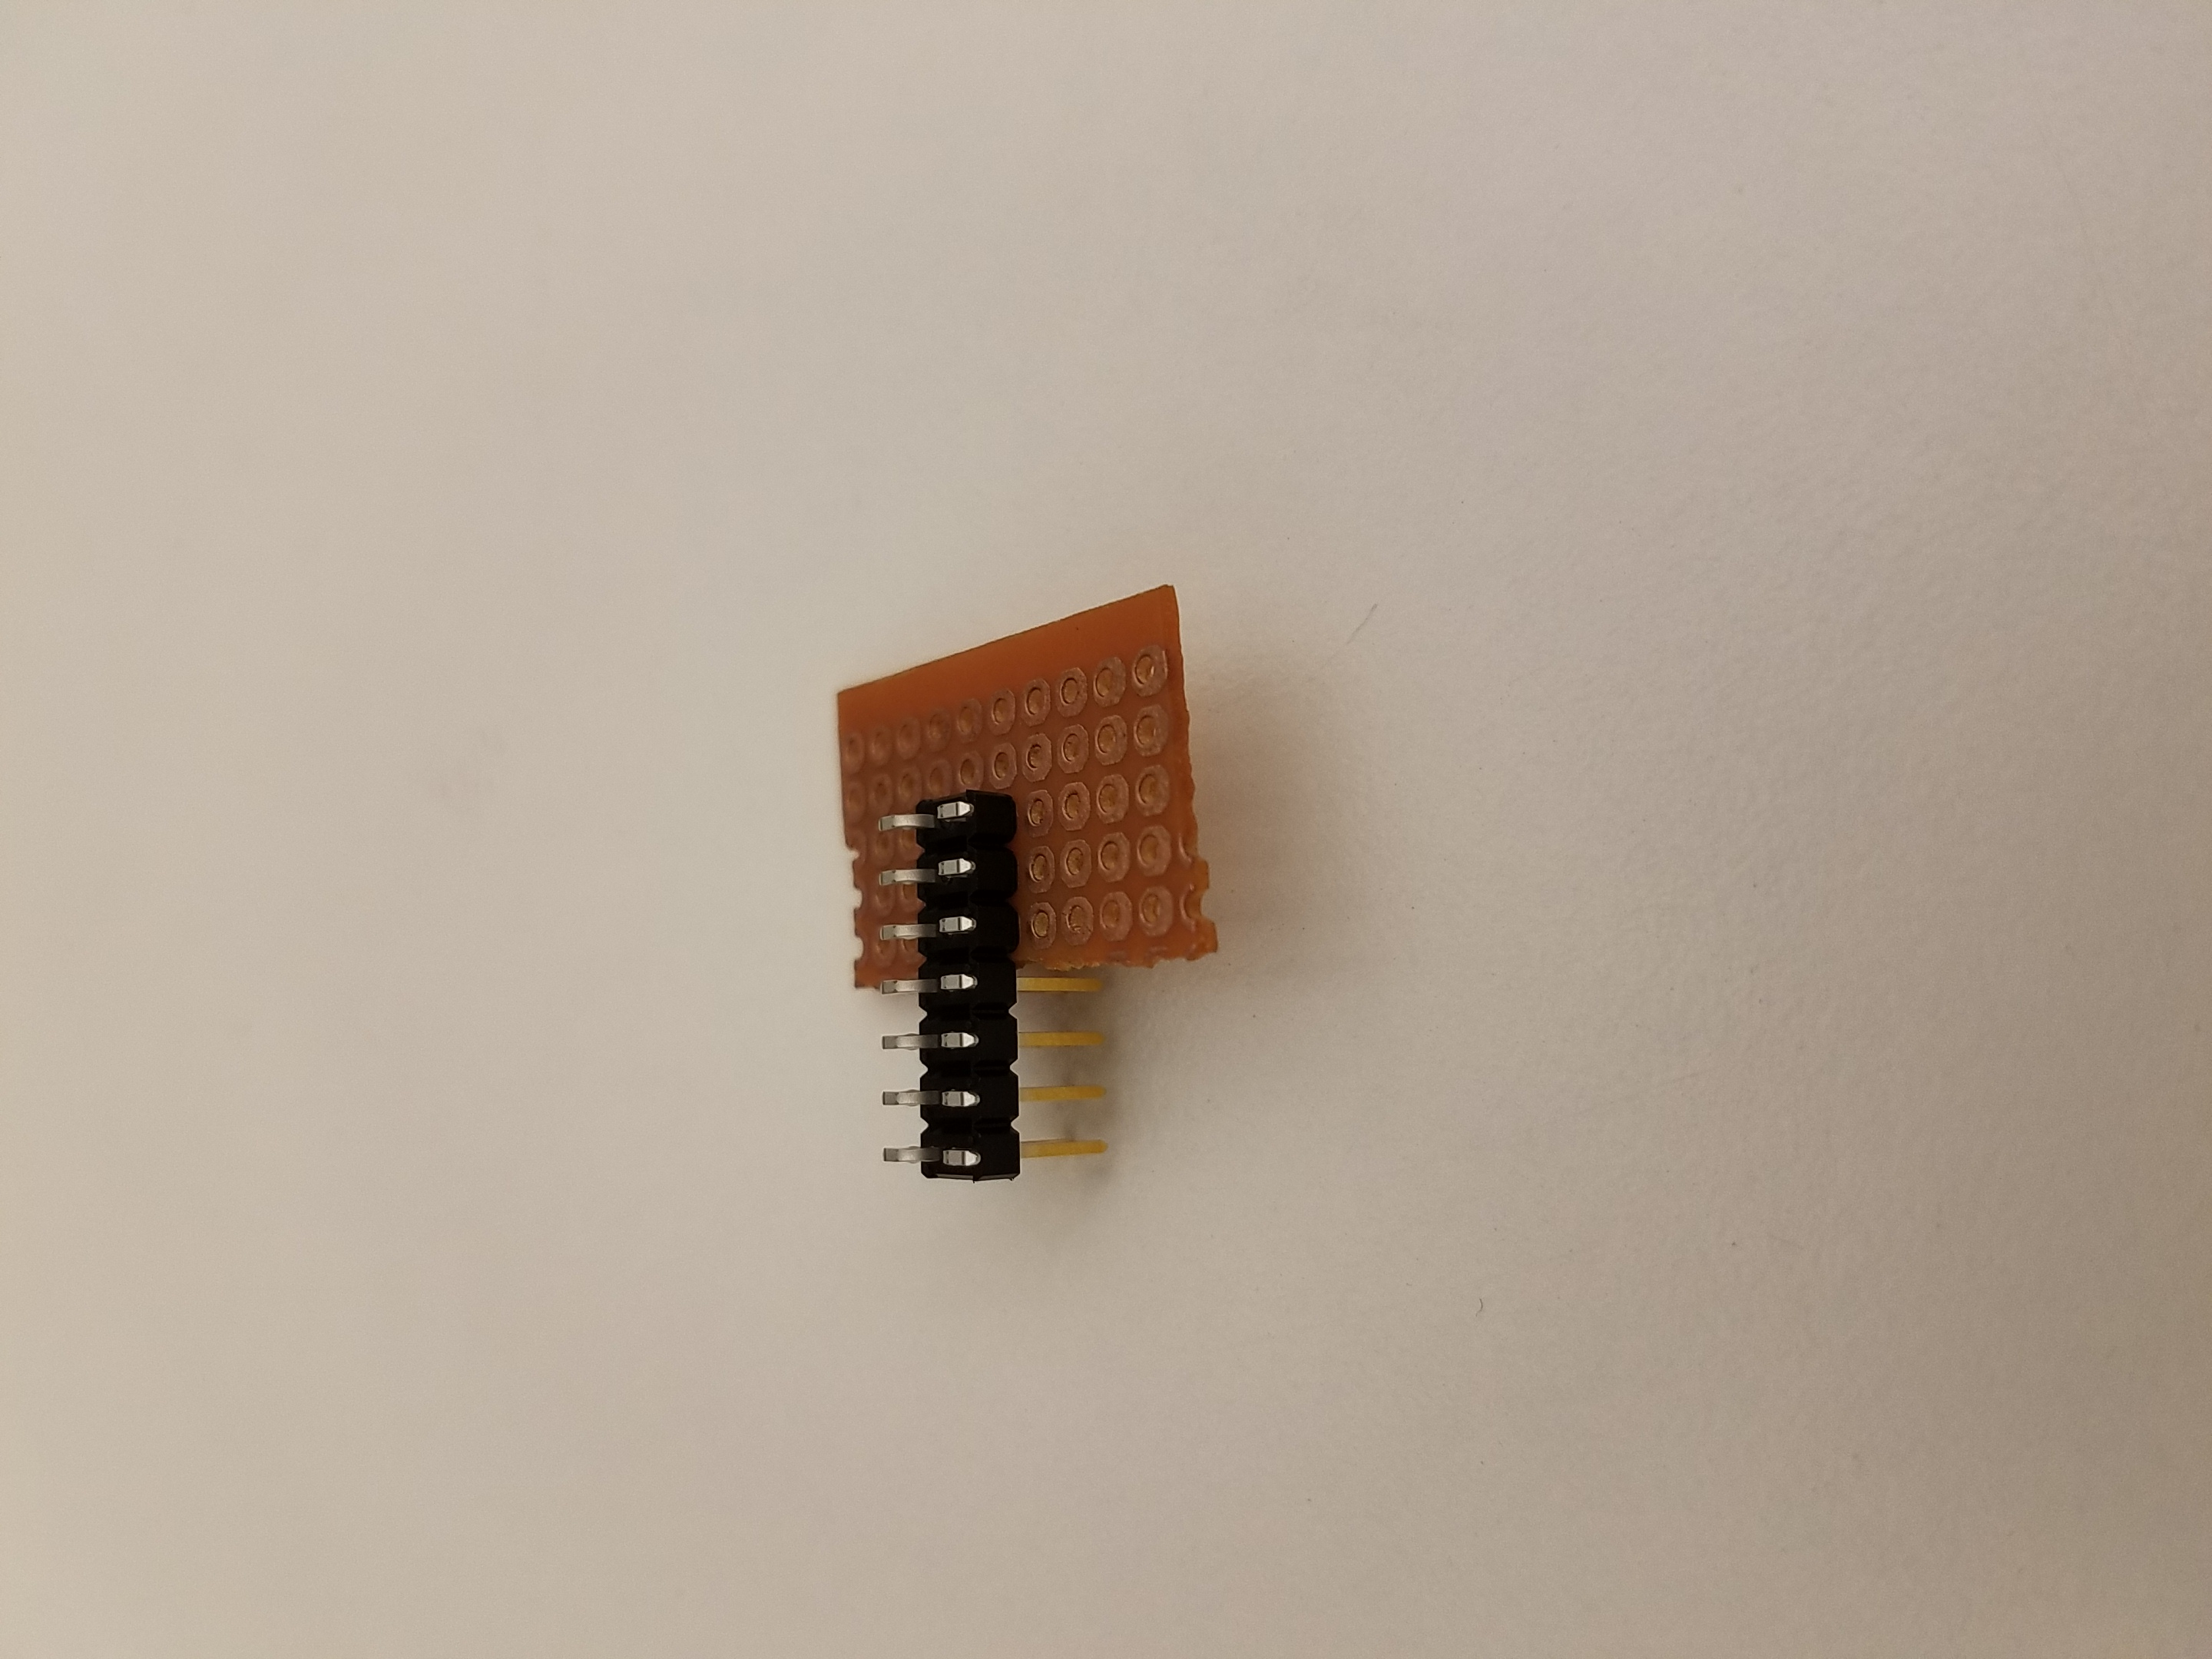
\includegraphics[trim={25cm 15cm 30cm 15cm},clip=true,width=0.45\columnwidth, keepaspectratio]{./figs/20180911_105607.jpg}}
\hfill
\subfloat[\label{fig:surfaceHeaderPerfTeensy}]{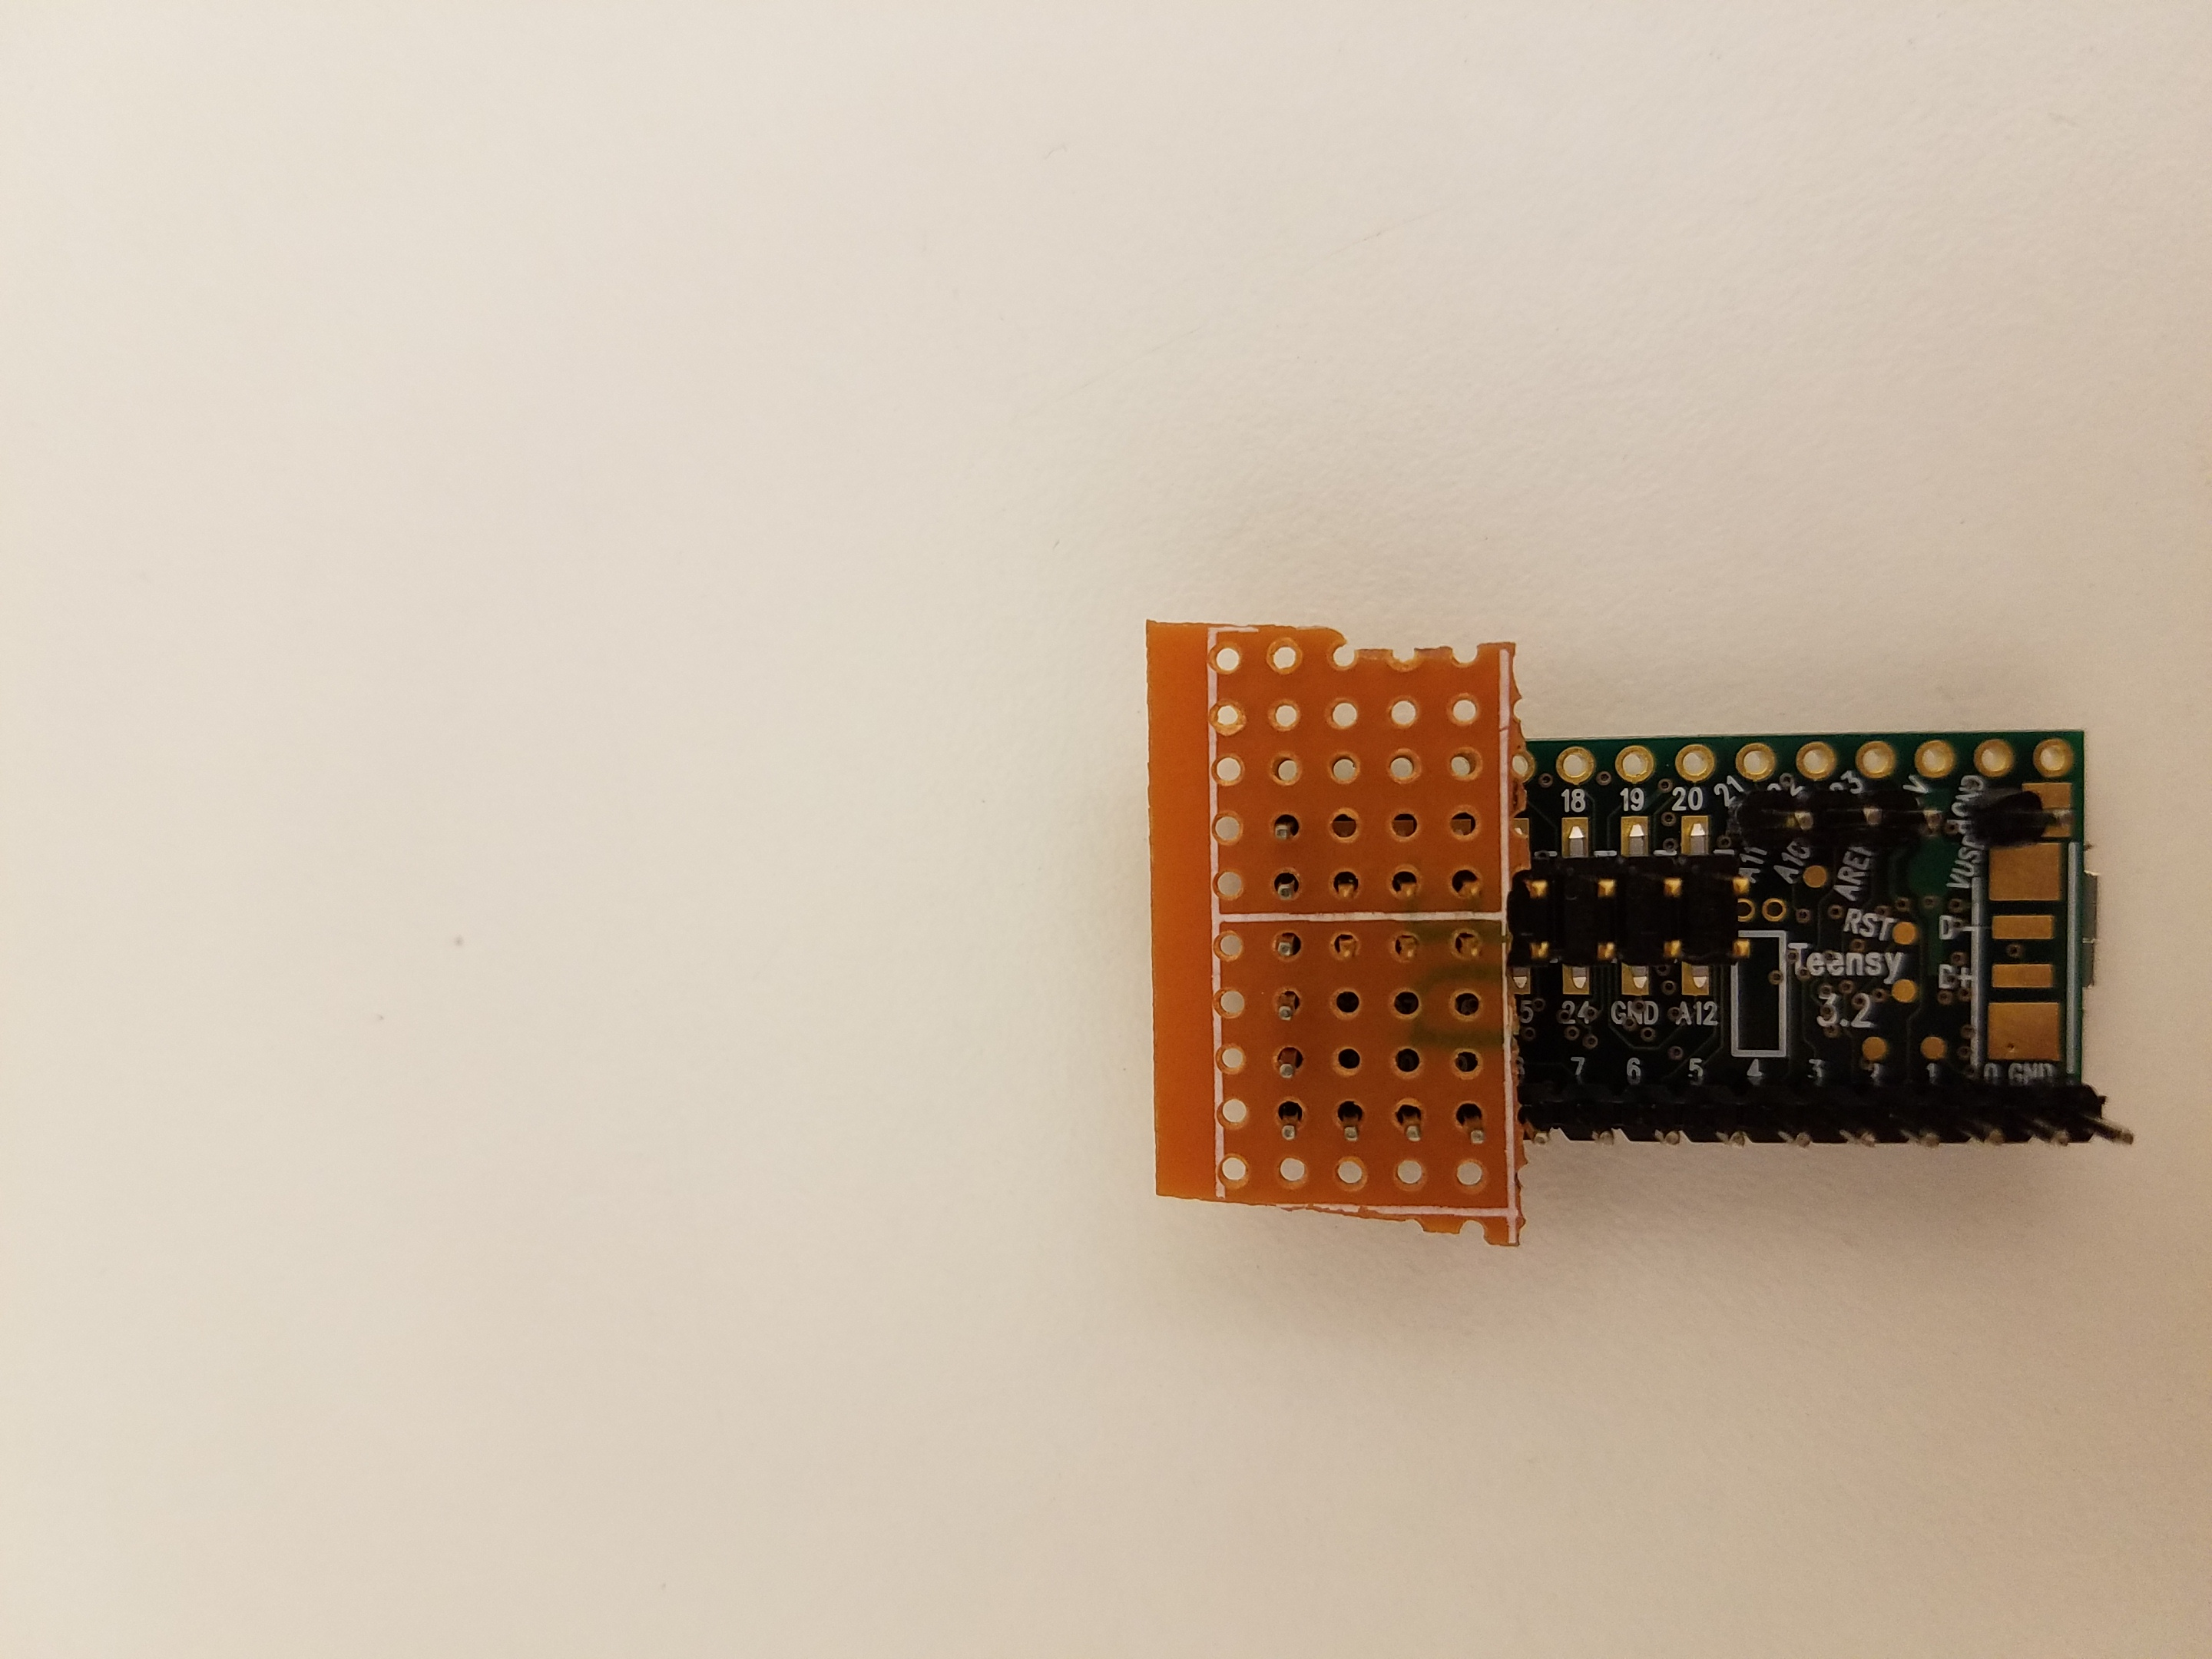
\includegraphics[trim={45cm 0 0 10cm},clip=true,width=0.445\columnwidth, keepaspectratio,angle=270,origin=br]{./figs/20180911_105641.jpg}}\\
\subfloat[\label{fig:surfaceHeaderTeensy}]{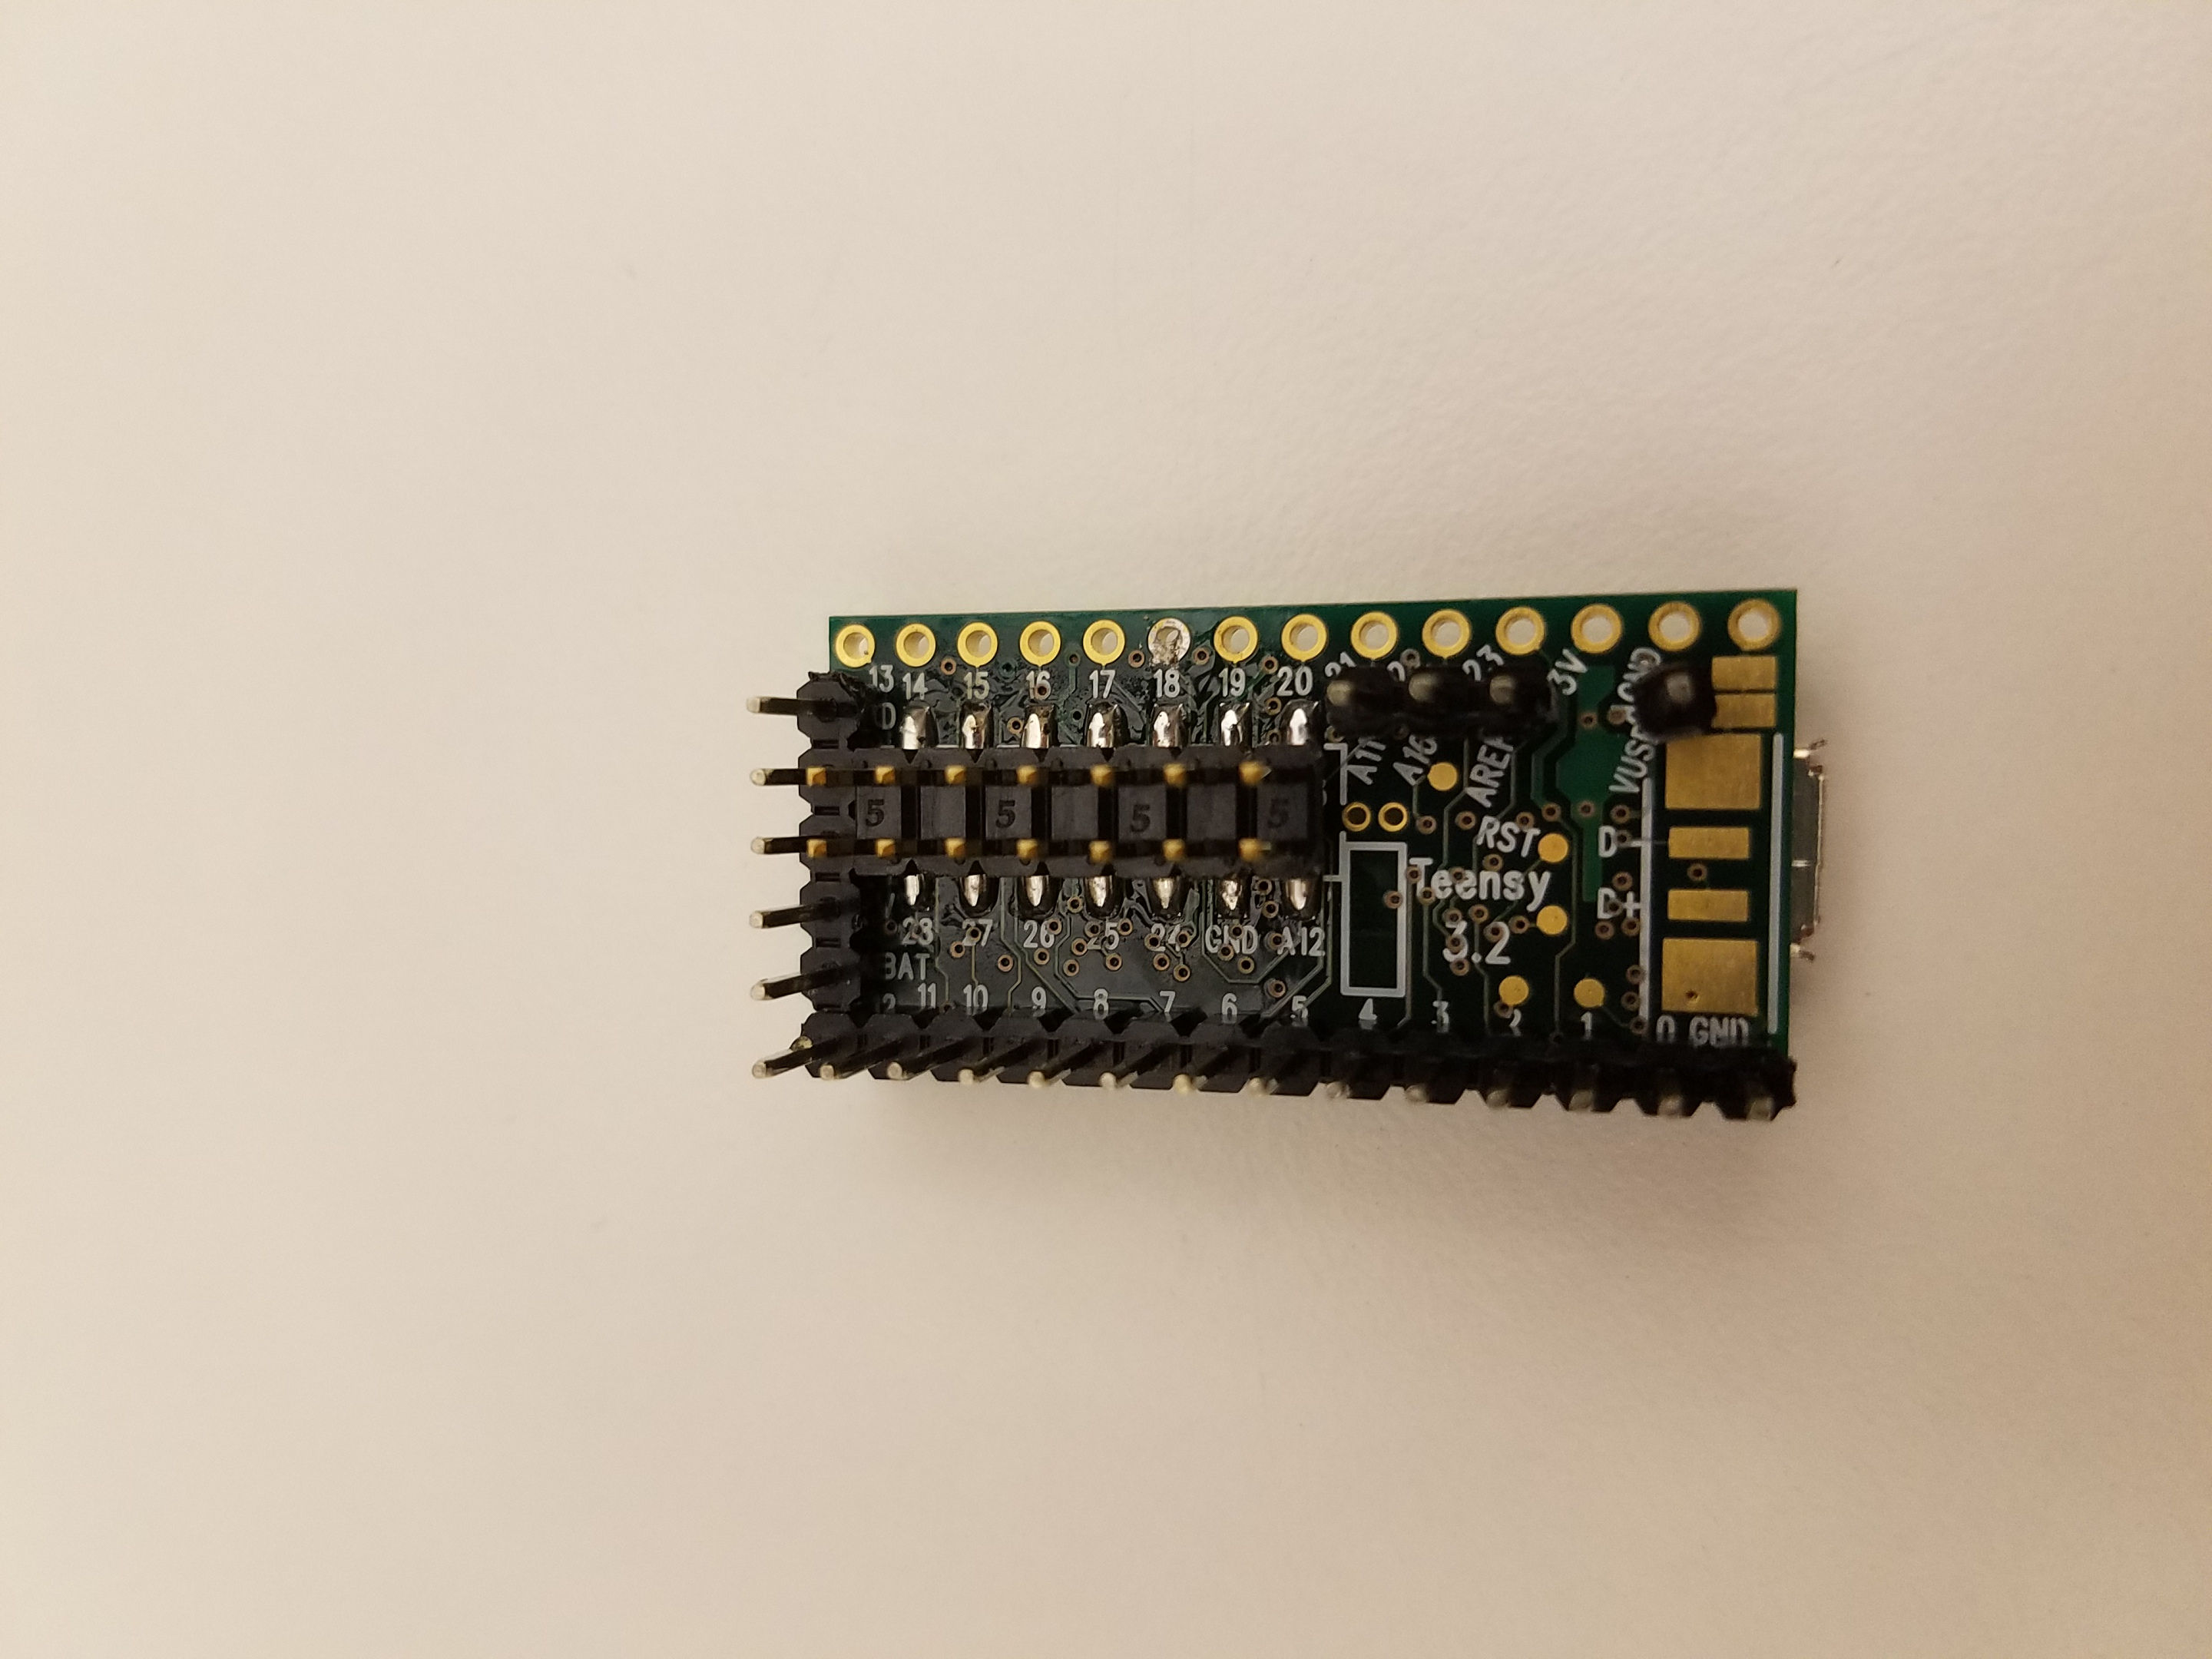
\includegraphics[trim={15cm 0 0 0},clip=true,width=0.45\columnwidth, keepaspectratio,angle=270,origin=br]{./figs/20180911_110201.jpg}}
\caption{Aligning and soldering the surface mount headers for the Teensy.}
\label{fig:teesnySurfaceHeaderPerf}
\end{figure}
%End Male headers in PCB picture

%%%Second Solder Pass Subsection (Surface Mount)
\subsubsection{Finishing Soldering the Teensy}
\label{sec:teensyFinalSolder}

To finish the Teensy, insert it back into the main GRITSBot X PCB as a guide and solder the remaining male header pins on the left side of the board. \textbf{\textcolor{red}{Again, before soldering}}, observe the proximity of the header pads to the main processor chip (big black square) connections. When soldering be very careful not to accidentally solder or bridge these connections. It is best to keep the iron and solder being applied on the outside perimeter of the boards. After making the final solder connection, you're done! The top and bottom of the finished Teensy should look like \cref{fig:teensyFinished}. The Teensy microcontroller is ready to be permanently attached to the main PCB of the GRITSBot X. Check it for bridged connections or poor solder joints. For now, take the Teensy out of the main PCB of the GRITSBot and set it aside to be attached later.

 %Teensy Materials Surface Mount Picture
\begin{figure}[h!]
\centering
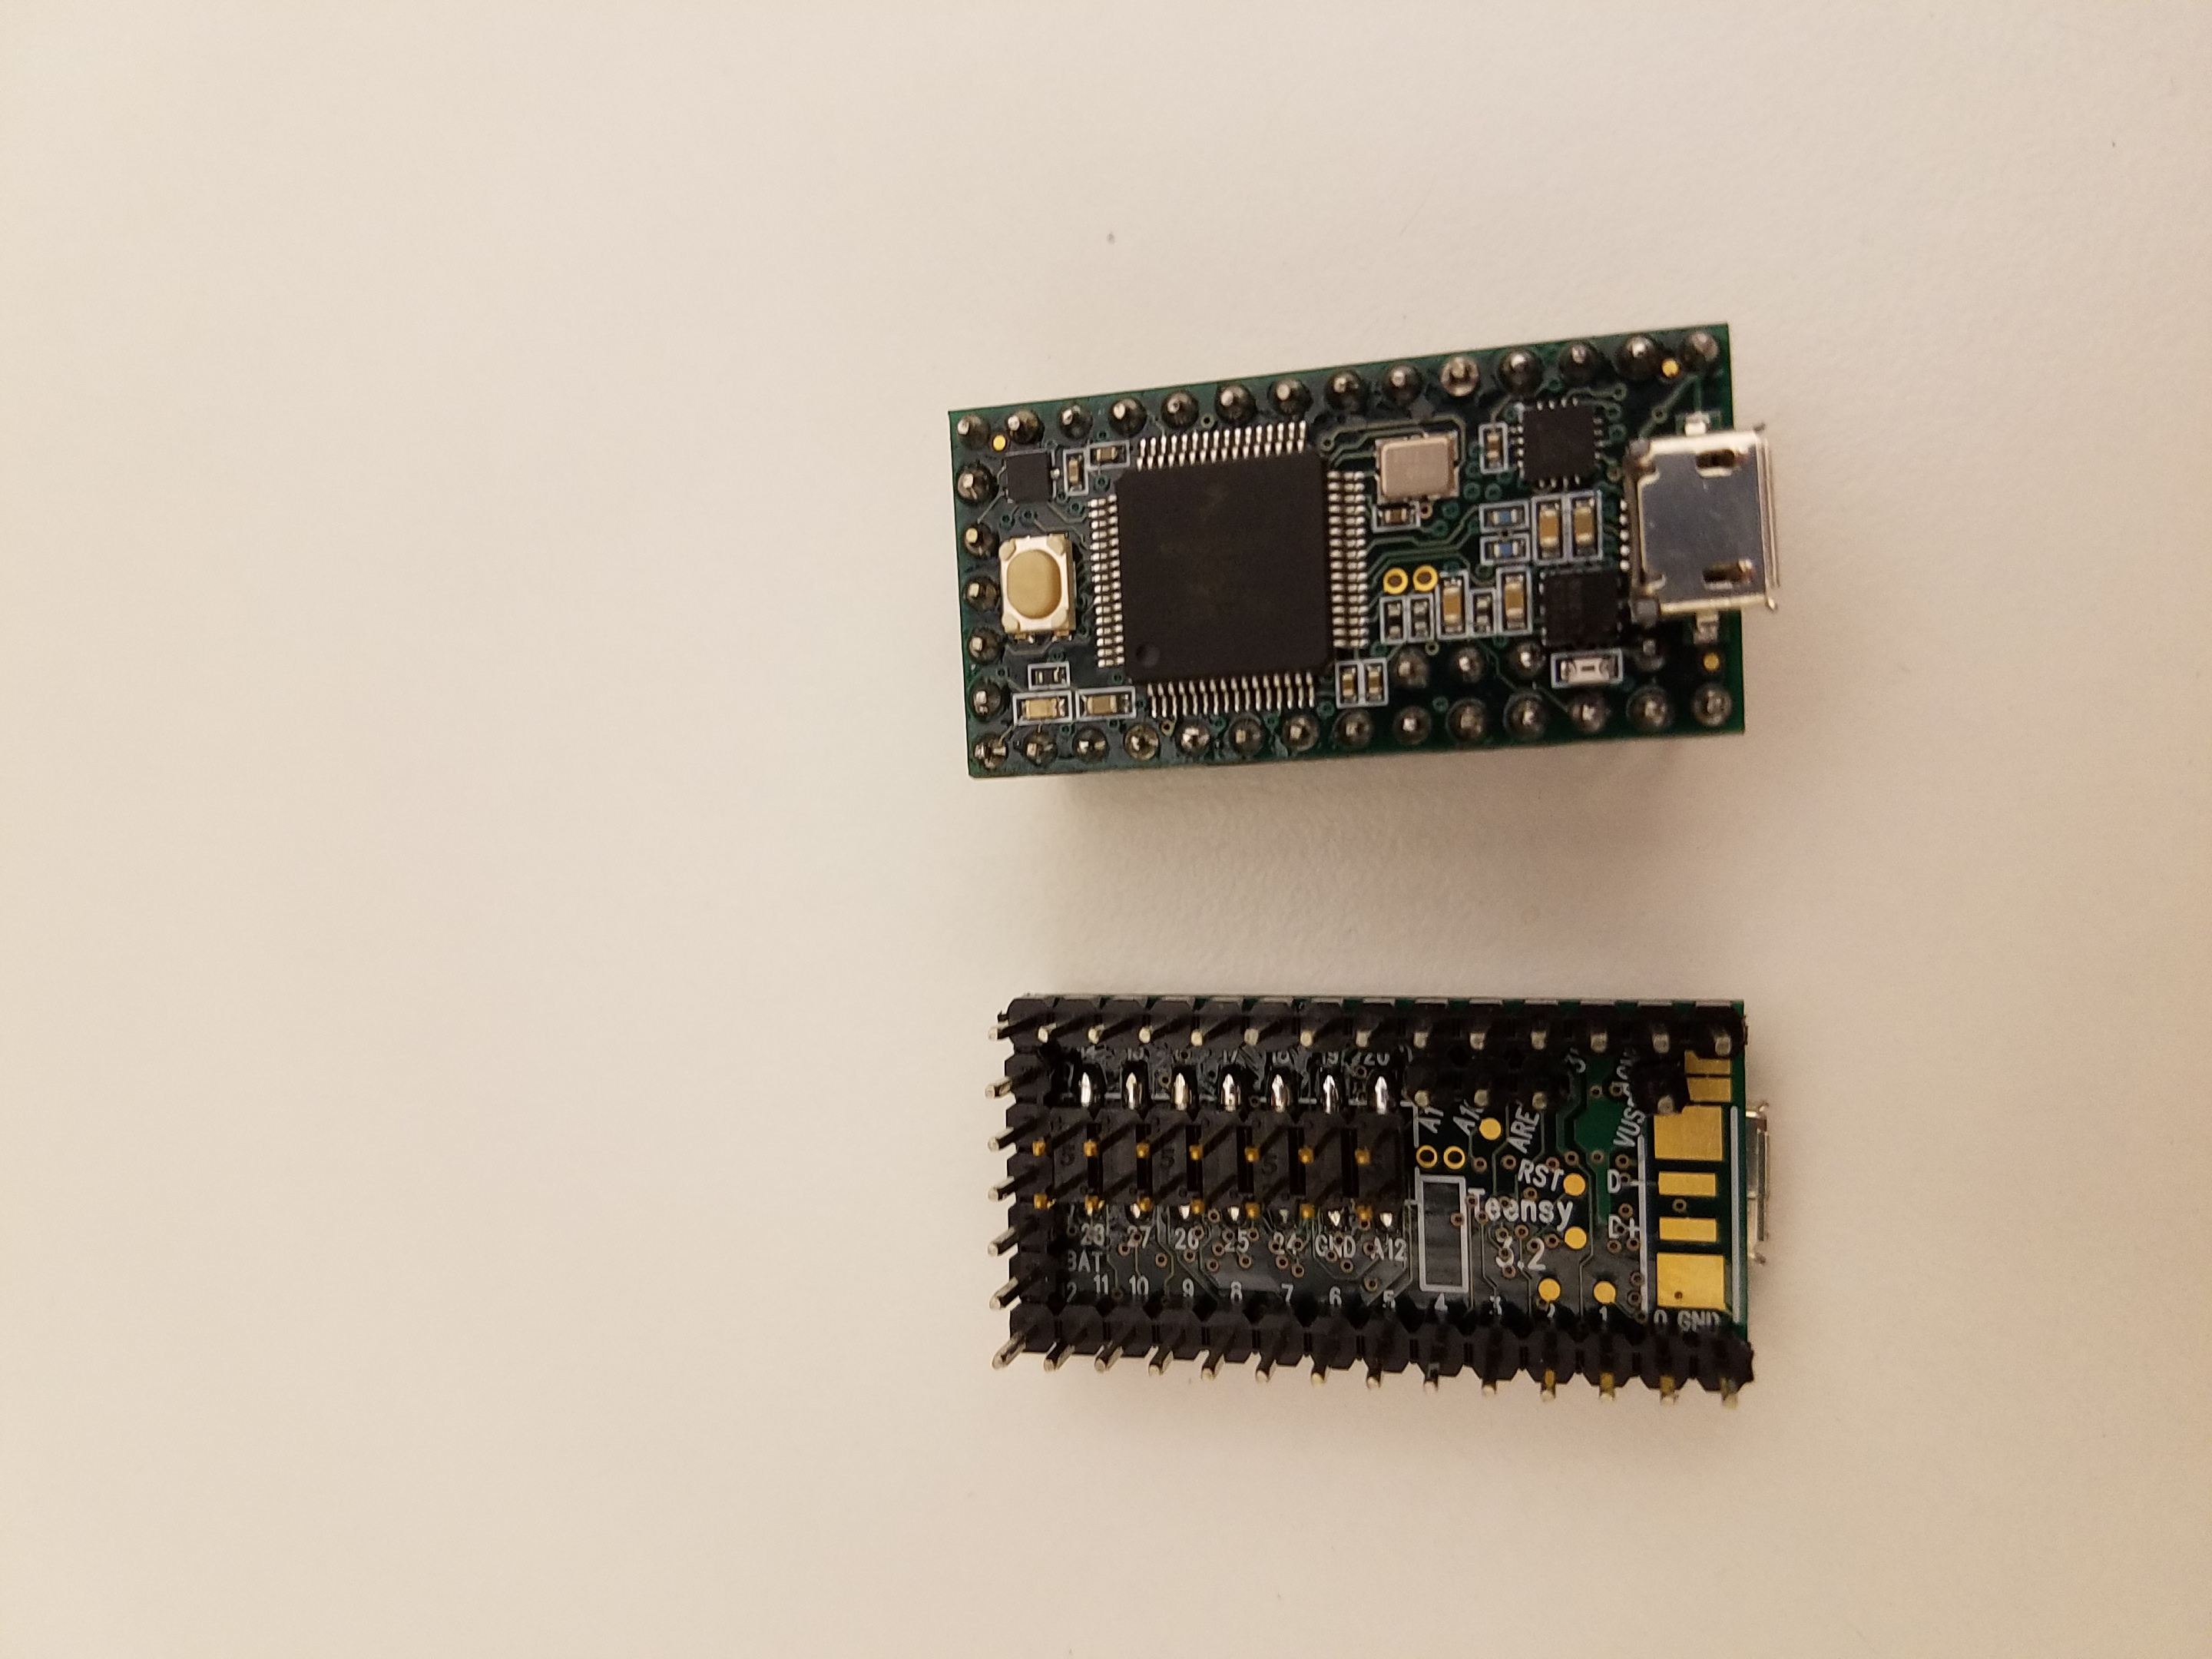
\includegraphics[trim={25cm 0 0 0},clip=true,width=0.65\columnwidth, keepaspectratio,angle=270]{./figs/20180912_111949.jpg}
\caption{The Teensy with headers attached.}
\label{fig:teensyFinished}
\end{figure}
%End Teensy Materials Surface Mount Picture  

\subsection{Pololu Carrier with Sharp GP2Y0A60SZLF Analog Distance Sensor}

 \subsubsection{Assembly Steps}
 
 \begin{enumerate}
 \item Gather the required materials (\cref{sec:sharpMaterials}).
 \item Cut the IR sensor down to size (\cref{sec:cutSharp}).
 \item Solder the right angle male header pins (\cref{sec:sharpSolder}).
 \end{enumerate}
 
  %%% Sharp Materials Subsection
 \subsubsection{Required Materials}
 \label{sec:sharpMaterials}
 
 Pololu provides the sensor attached to a custom PCB, male breakaway header pins, and right angle breakaway male header pins as seen in \cref{fig:sharpMaterials}. Only the sensor and right angle breakaway male header pins are needed for this. This means the normal breakaway header pins may be used for other projects (or for populating the VUSB pin on the Teensy).
 
 The GRITSBot X uses seven of these sensors so we require seven of these kits and soldering described below will have to be performed on each of the sensors.
 
 %Sharp Materials Picture
\begin{figure}[h!]
\centering
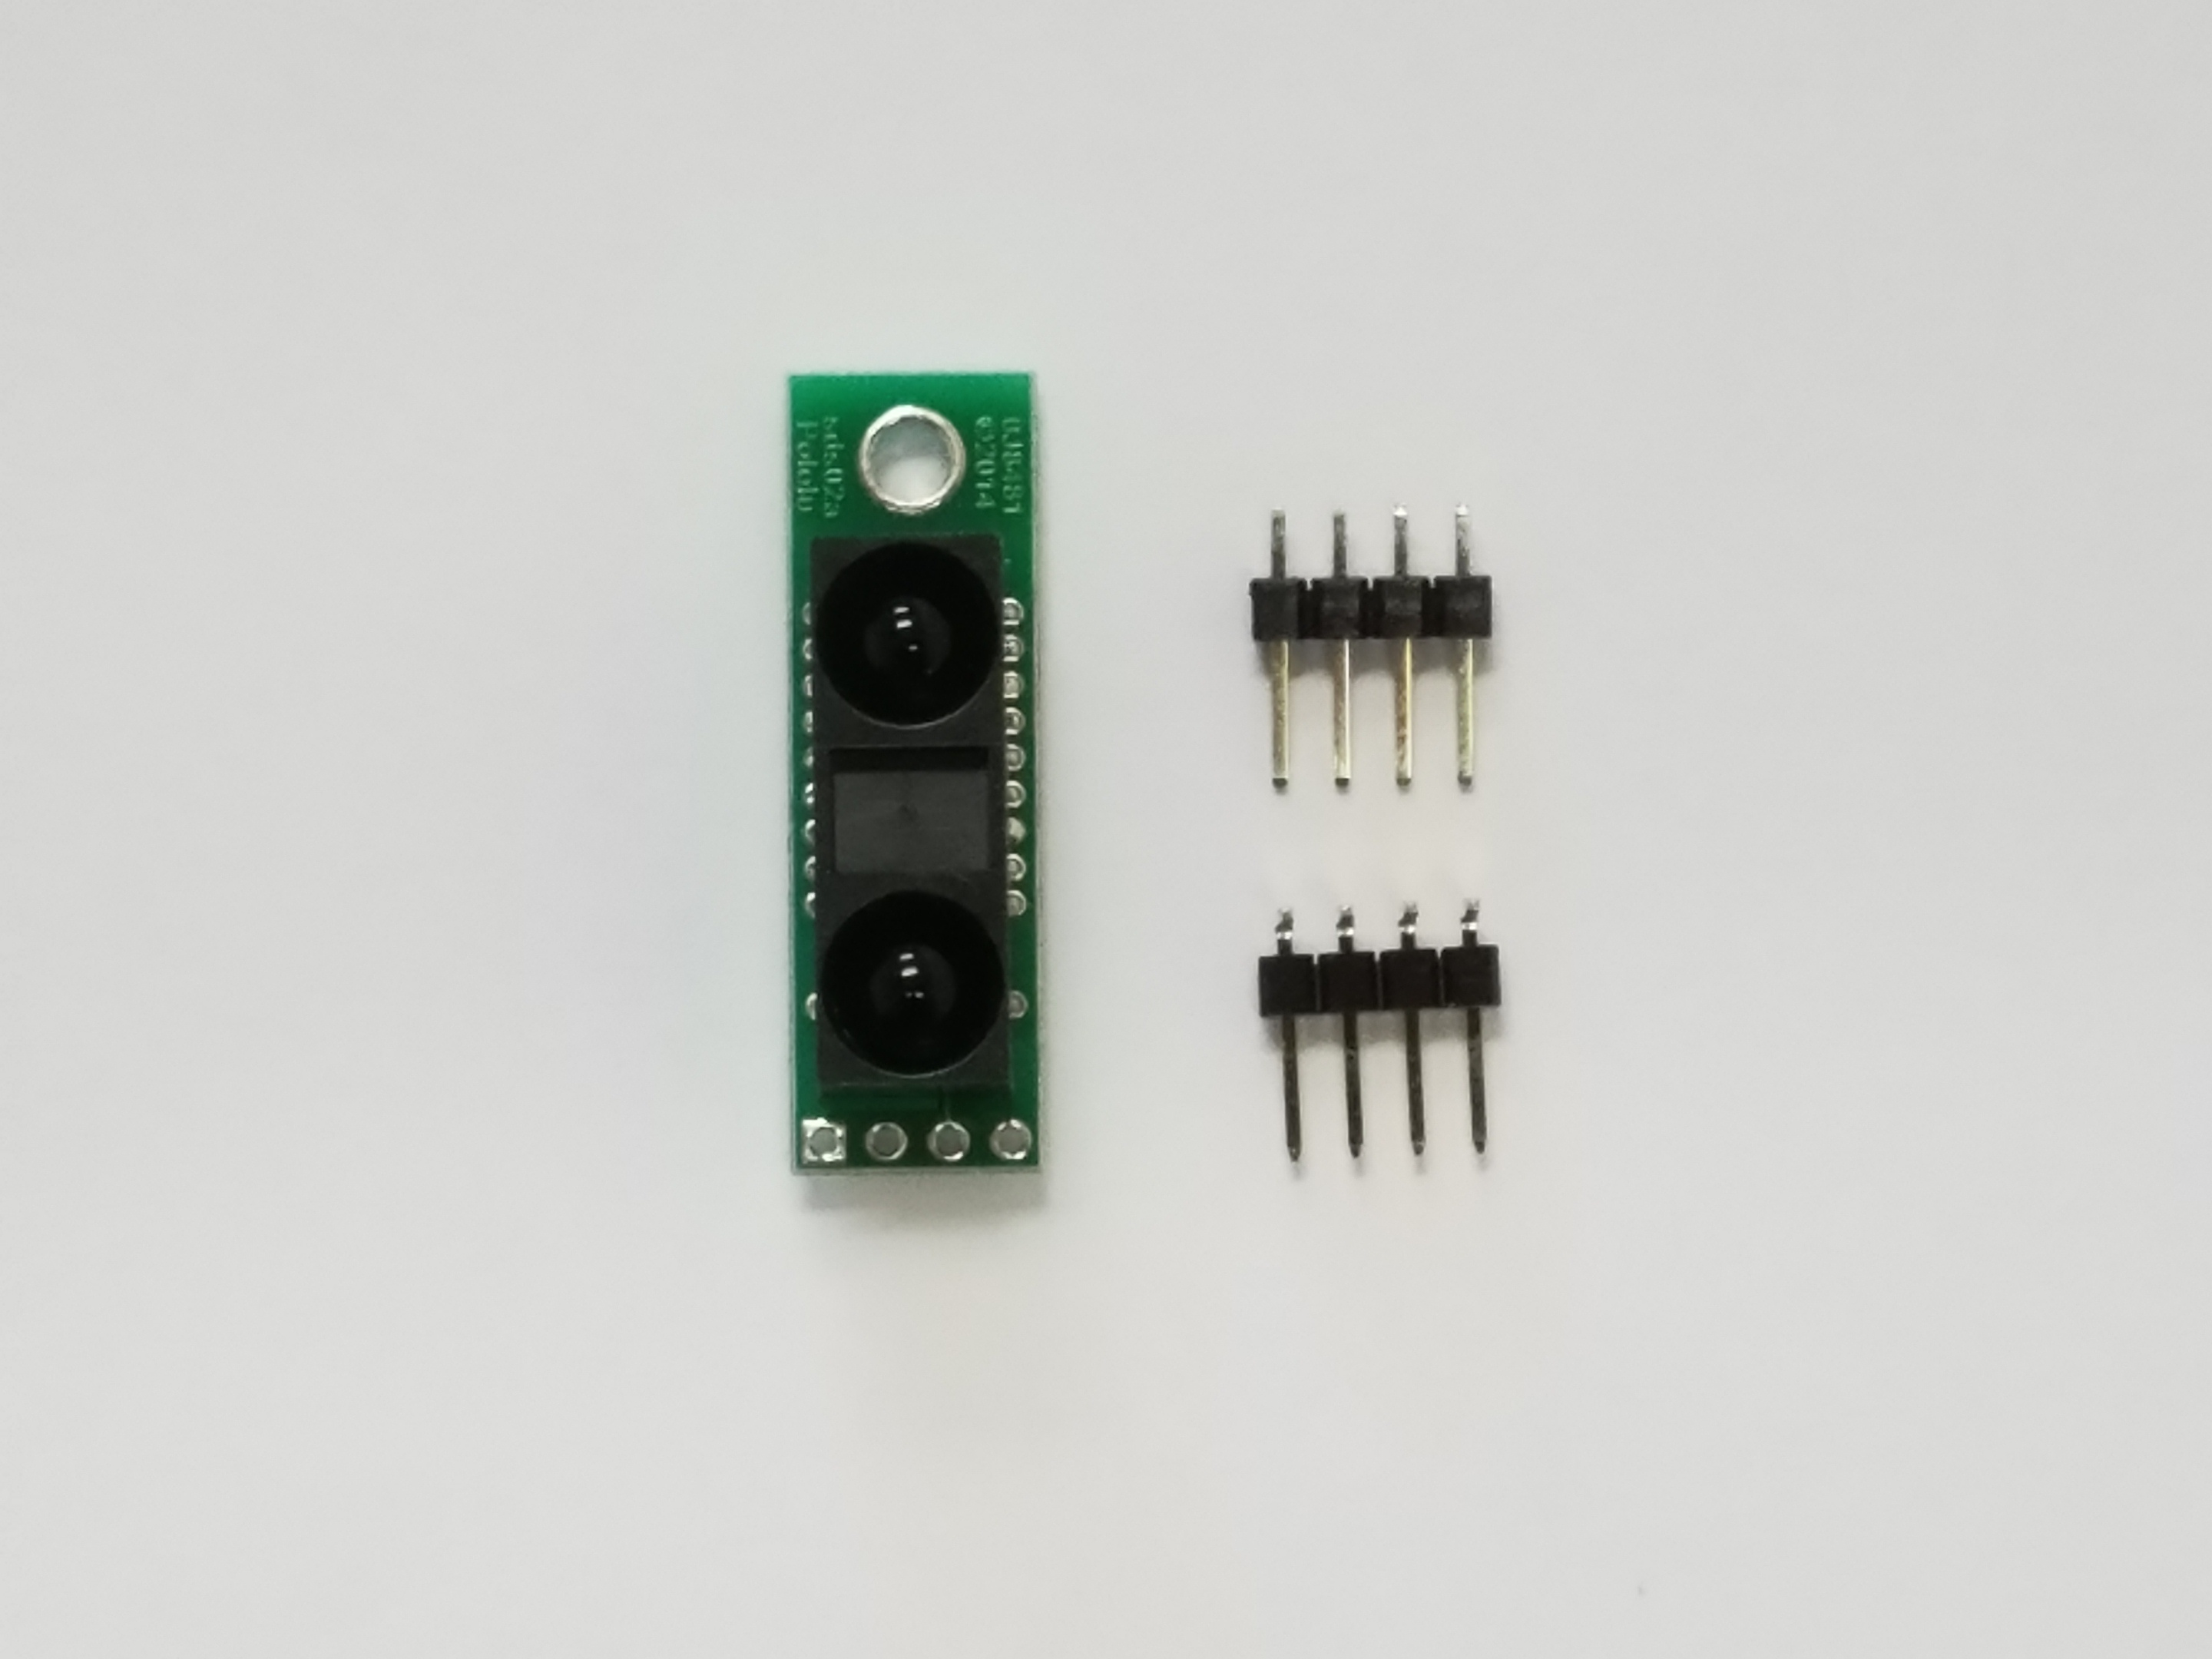
\includegraphics[width=0.65\columnwidth, keepaspectratio]{./figs/20181121_110942.jpg}
\caption{The materials required to assemble the Sharp infra-red piggyback board.}
\label{fig:sharpMaterials}
\end{figure}
%End Sharp Materials Picture  

 \subsubsection{Cutting the Pololu Carrying Board}
 \label{sec:cutSharp}
 
 The Pololu carrying board, that supports the Sharp IR sensor used on the robot, comes with a screw mounting hole that we do not use for this robot. In order to keep the robot's center of gravity low, we must cut the excess PCB used for a screw mount. The aim is to make a flat cut right below the plastic black sensor casing where the screw hole is. There are a few ways to do this. This guide will discuss three options with their drawbacks,
 
 \begin{itemize}
 \item Use a pair of scizzors to cut the boards. This is the most time efficient and safe way to do this. The drawback is that it can be hard on your hands so wear gloves or take breaks between large amounts of cuts (if you are mass producing).
 \item Use a box cutter to slice at each side and then snap the board along the weakened line. This is agin relatively safe but you have a higher chance of cutting yourself. This method is also rather time consuming.
 \item Use a dremel or other machine cutter to cut the board. This method works but is not recommended unless the above two fail. {\textcolor{red}{NOTE}}: this will create dust that is possibly hazardous so wear breath protection. You should also place the sensor into a vice or some other type of holder. Do not hold it in your hand as the dremel will most likely catch and you can BADLY hurt yourself.
 \end{itemize} 
 
  %Sharp Cut Picture
\begin{figure}[h!]
\centering
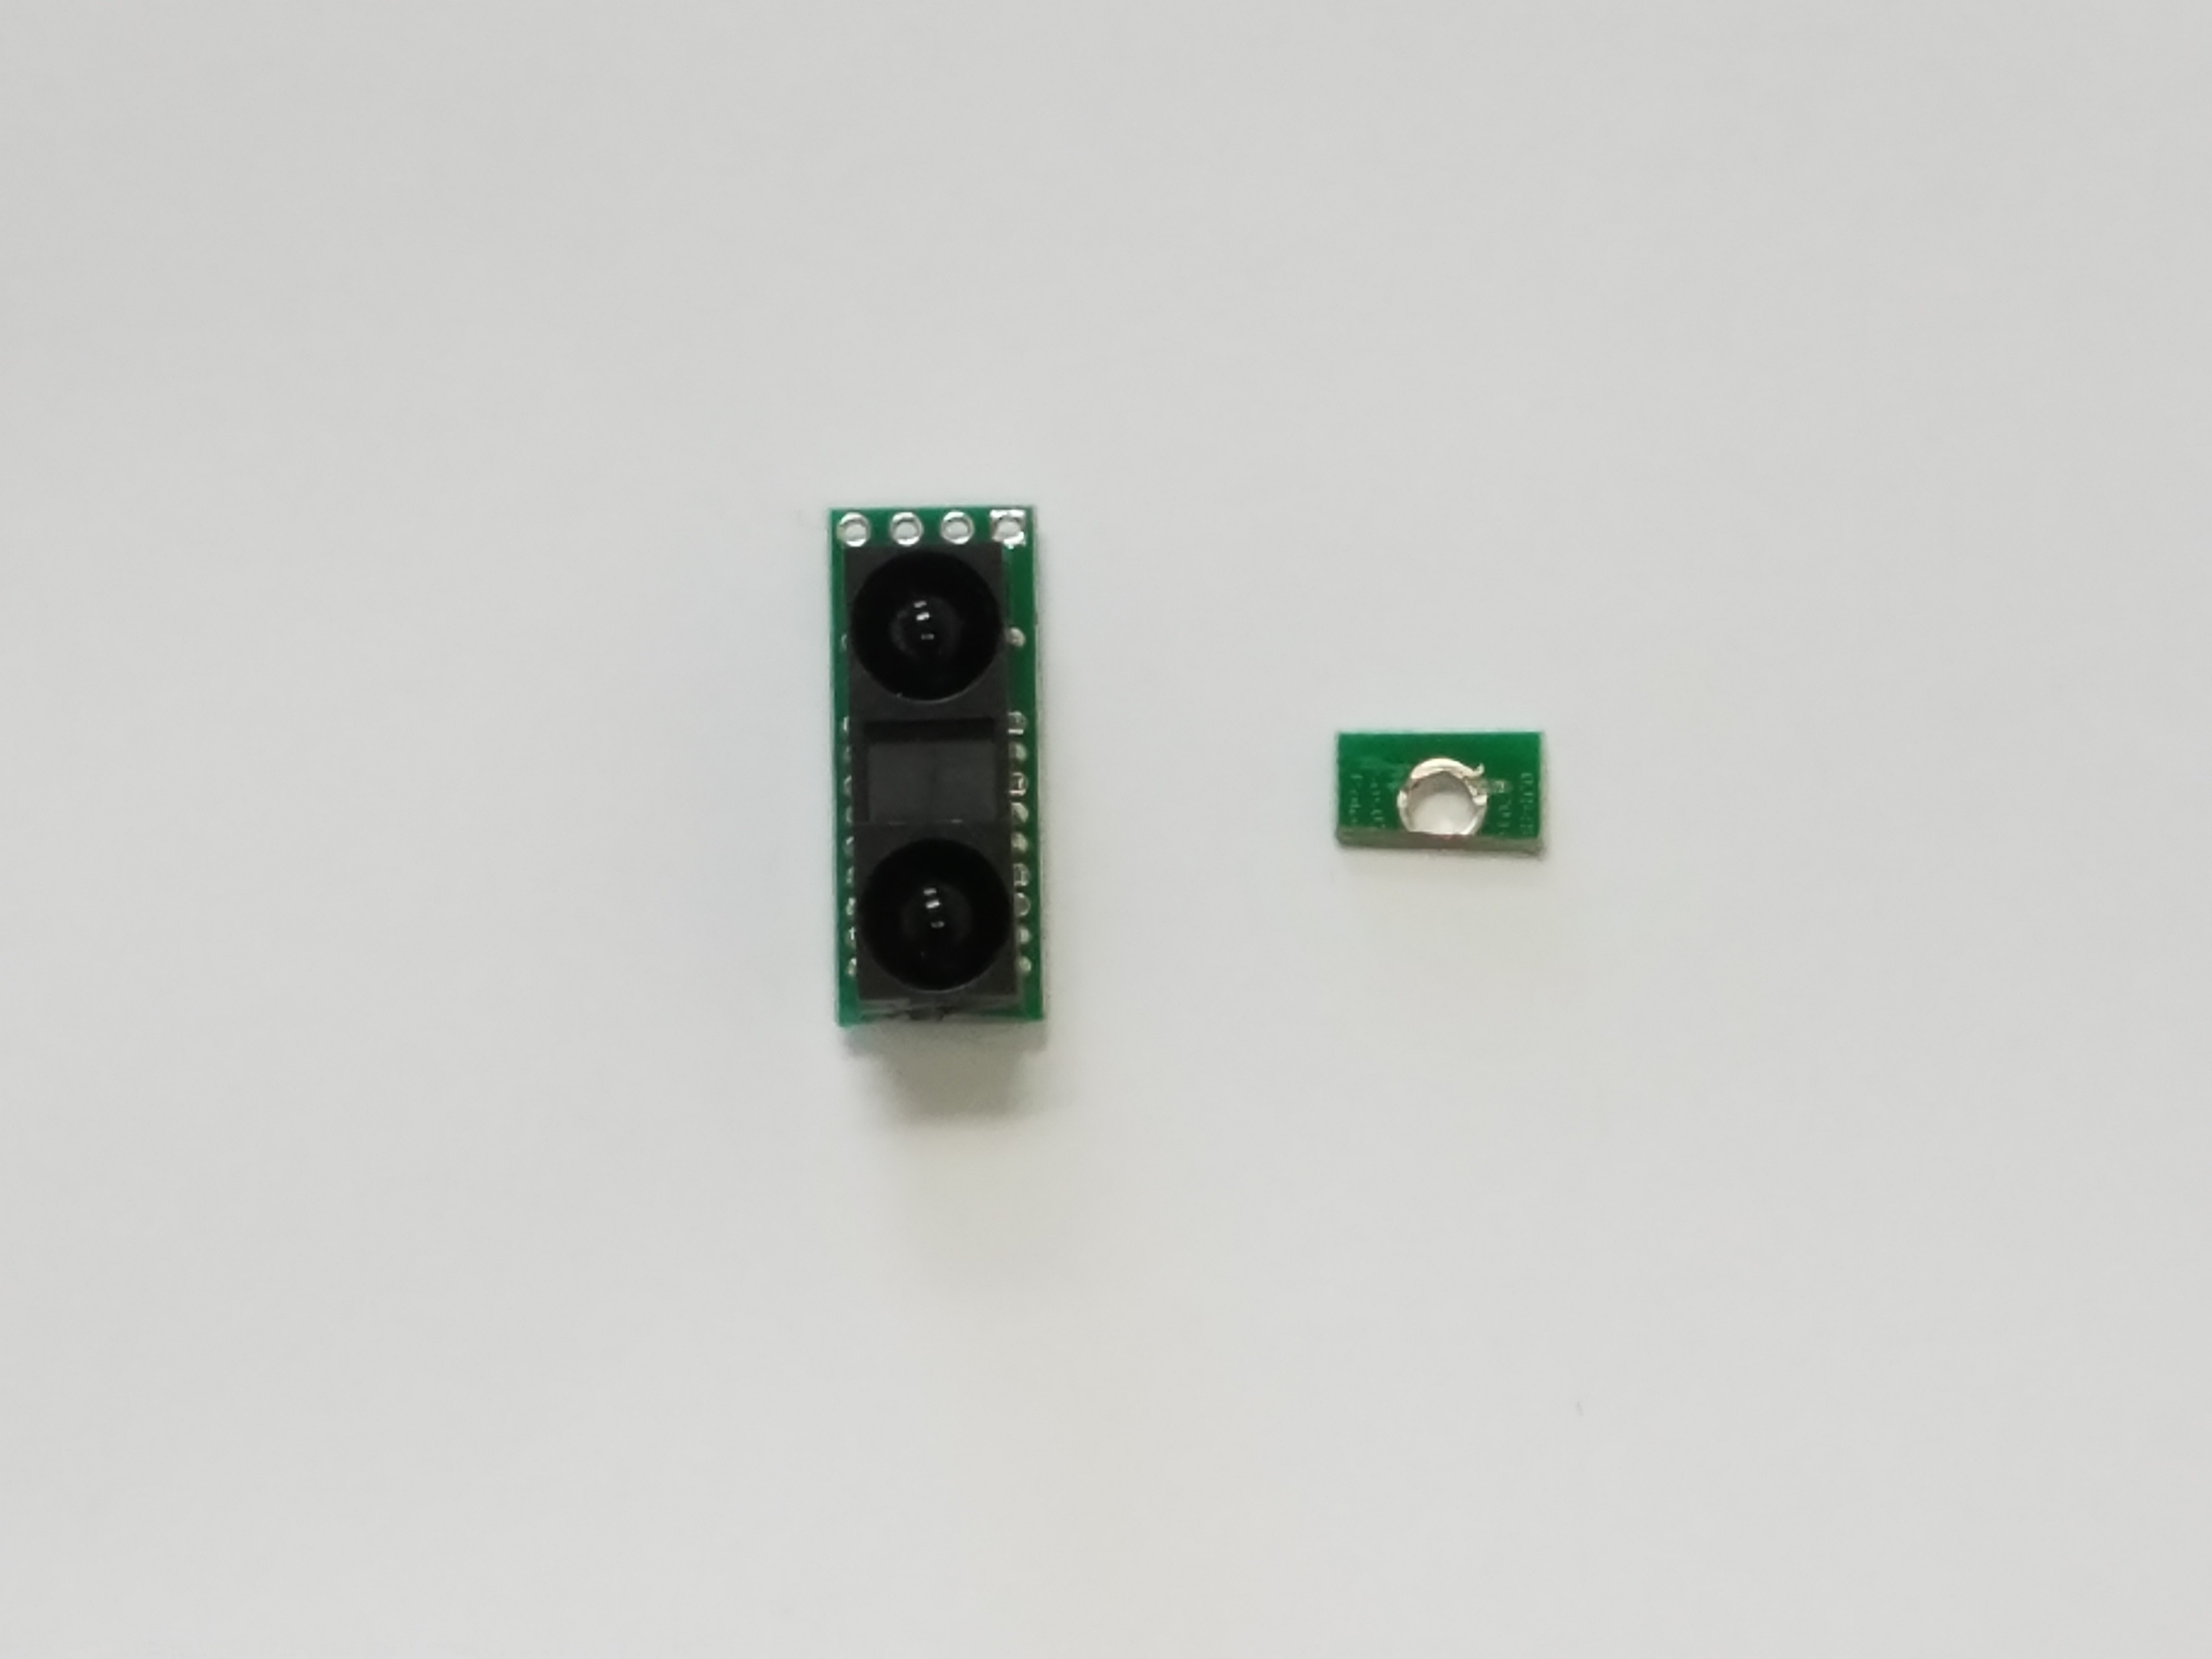
\includegraphics[trim={15cm 15cm 15cm 10cm},clip=true,width=0.65\columnwidth, keepaspectratio]{./figs/20181121_111015.jpg}
\caption{The Sharp IR sensor after being cut to size.}
\label{fig:cutSharp}
\end{figure}
%End Sharp Cut Picture

After cutting the sensor the sensor should look simlar to the one pictured in \cref{fig:cutSharp}.  
 
 %%% Sharp Soldering Subsection
 \subsubsection{Soldering the Header Pins}
 \label{sec:sharpSolder}
 
 Soldering the right angle breakaway header pins to this boards is relatively straight forward. However, it is important to make these solder joints as perpendicular to the board as possible. To do this, first insert the long straight section of the breakaway header through the back of the board such that the right angle pins are on the opposite side of the sensor (seen in \cref{fig:sharpHeaders}). Solder one pin connection. Lay the sensor face down and heat that connection while pushing the pins you are not heating (so you don't burn yourself) stright into the board such that they become perpendicular with the board. \textbf{\textcolor{red}{Careful}} not to leave the heat on this pin too long or you will melt the plastic holding it and cause misalignment of the right angle pins. If this happens the IR sensor cannot be inserted into the GRITSBot X's main PCB.
 
 After aligning the pins properly using the single solder point. Solder the rest of the pins and cut the excess with a wire cutter. The resulting sensor should look like \cref{fig:sharpFinished}.
 
%Male headers in PCB picture
\begin{figure}[h!]
\centering
\subfloat[\label{fig:sharpHeaders}]{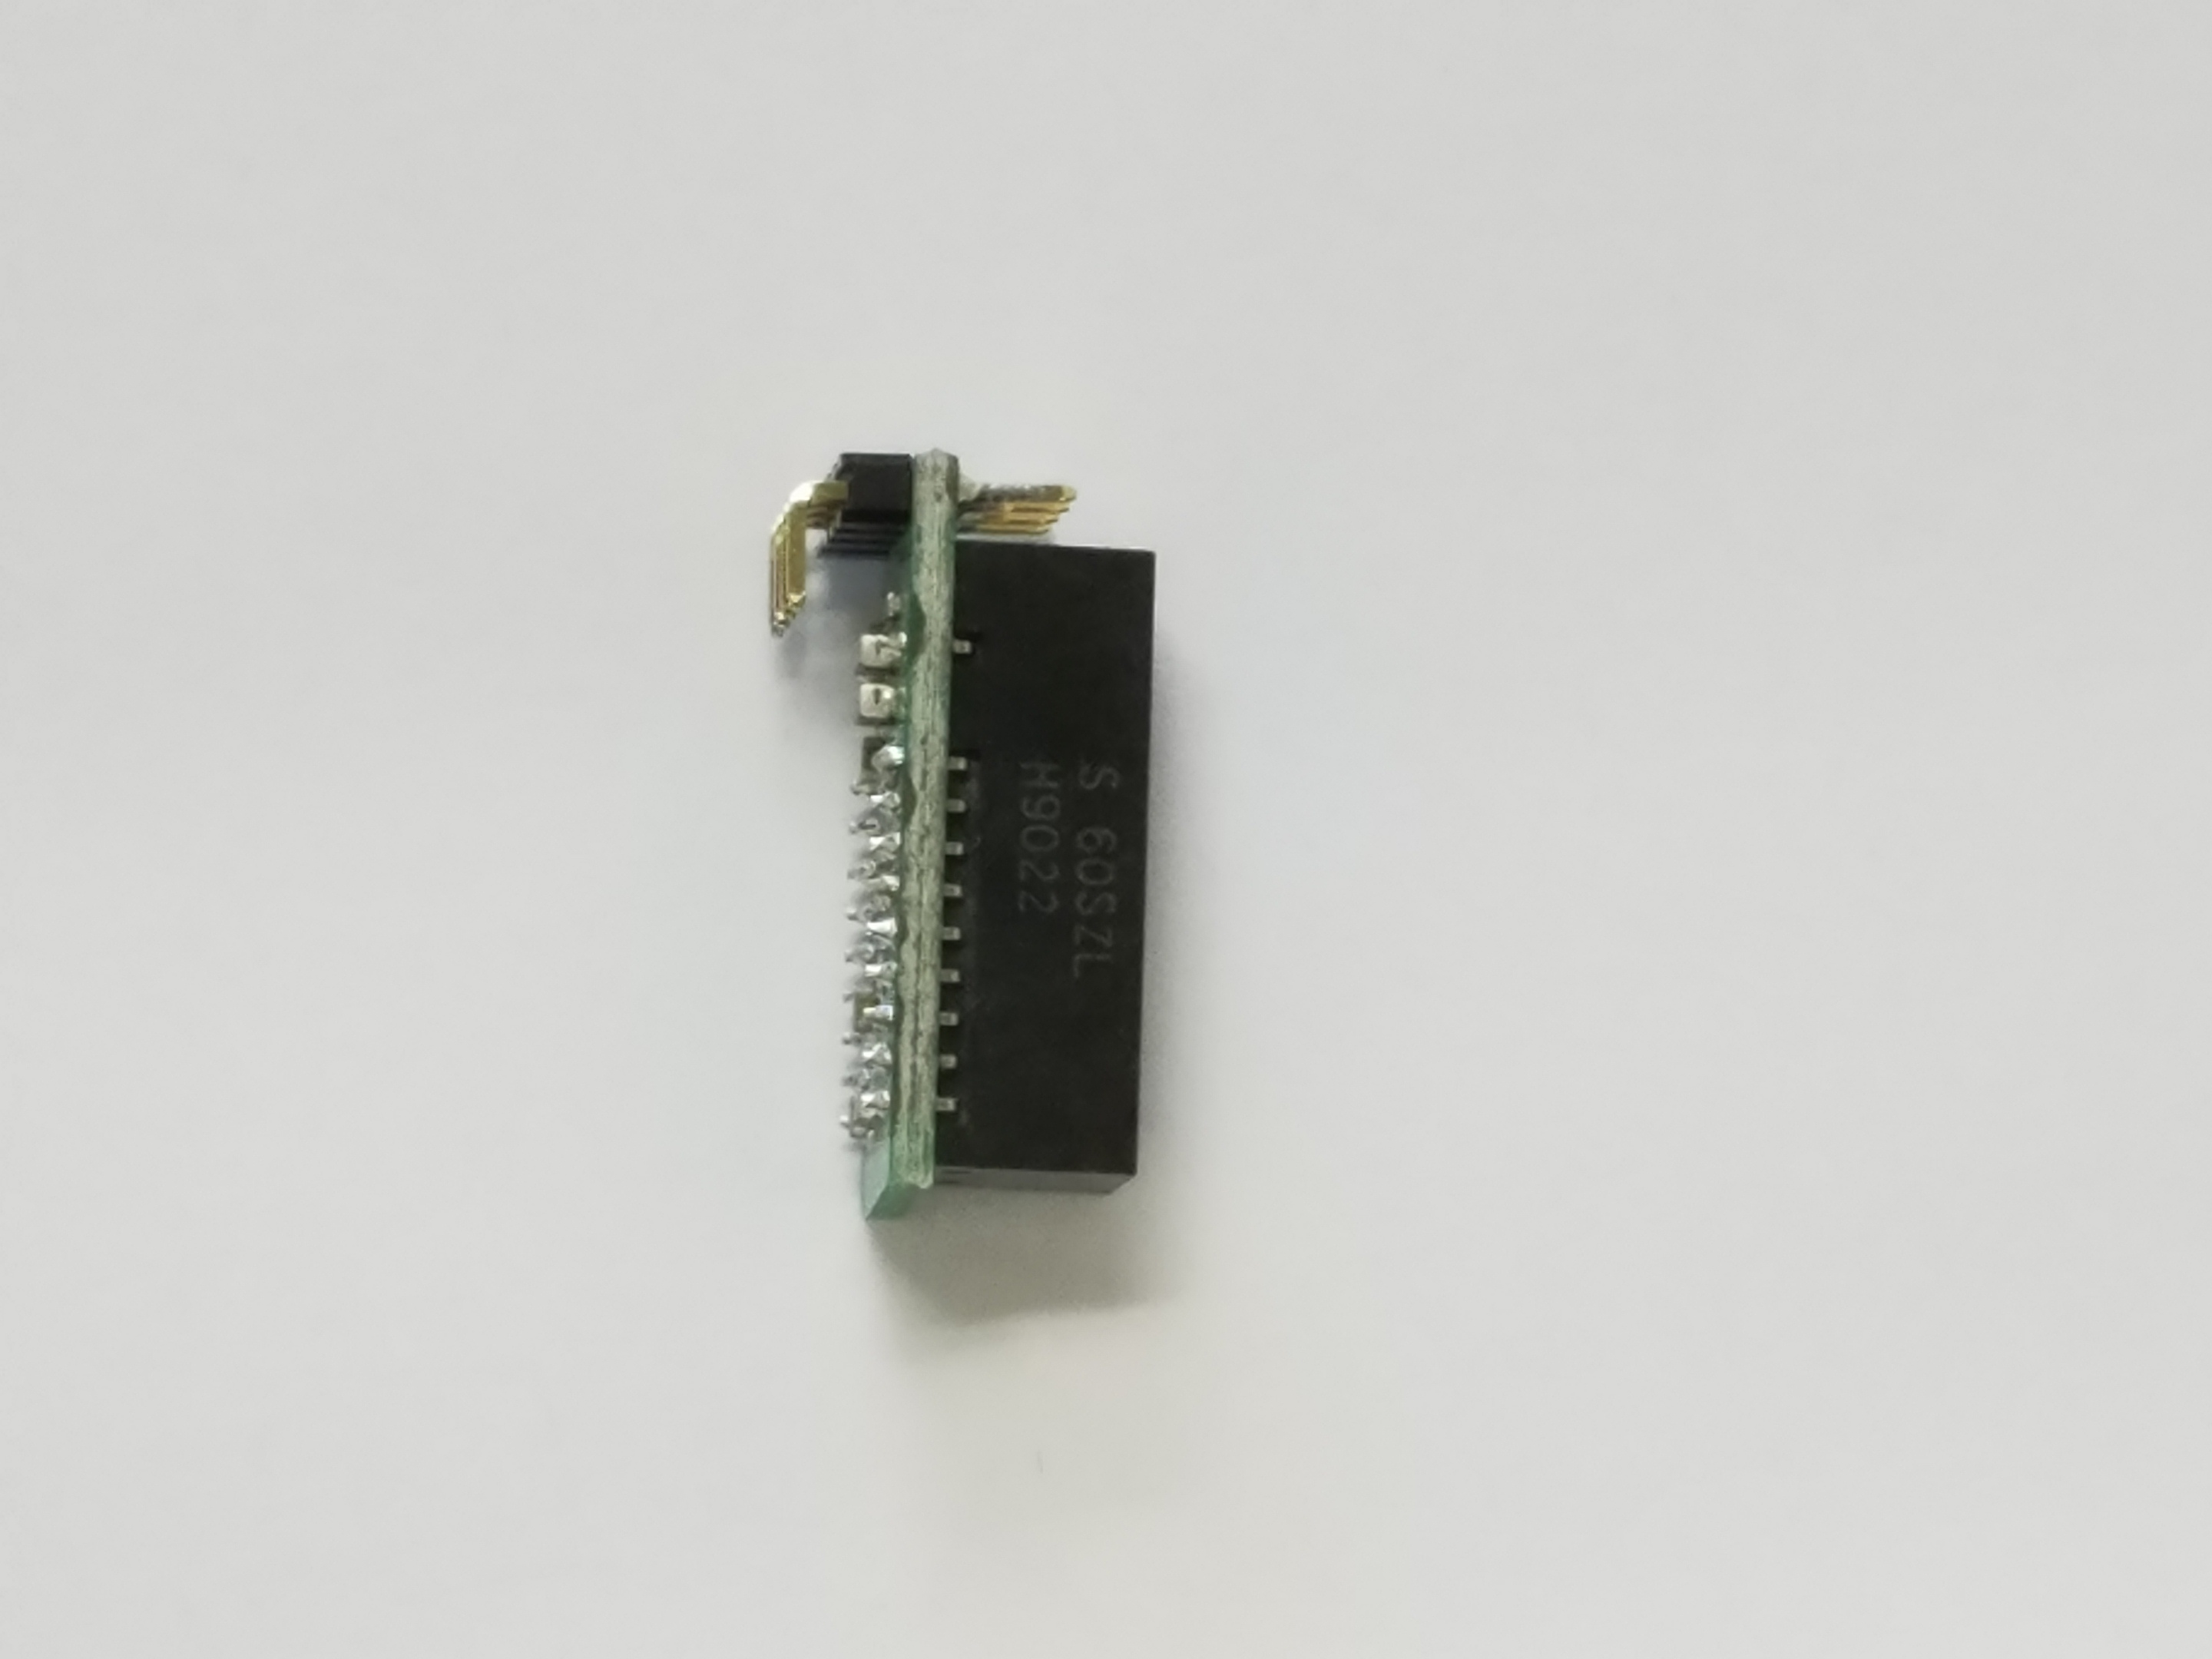
\includegraphics[width=0.45\columnwidth, keepaspectratio]{./figs/20181121_111512.jpg}}
\hfill
\subfloat[\label{fig:sharpFinished}]{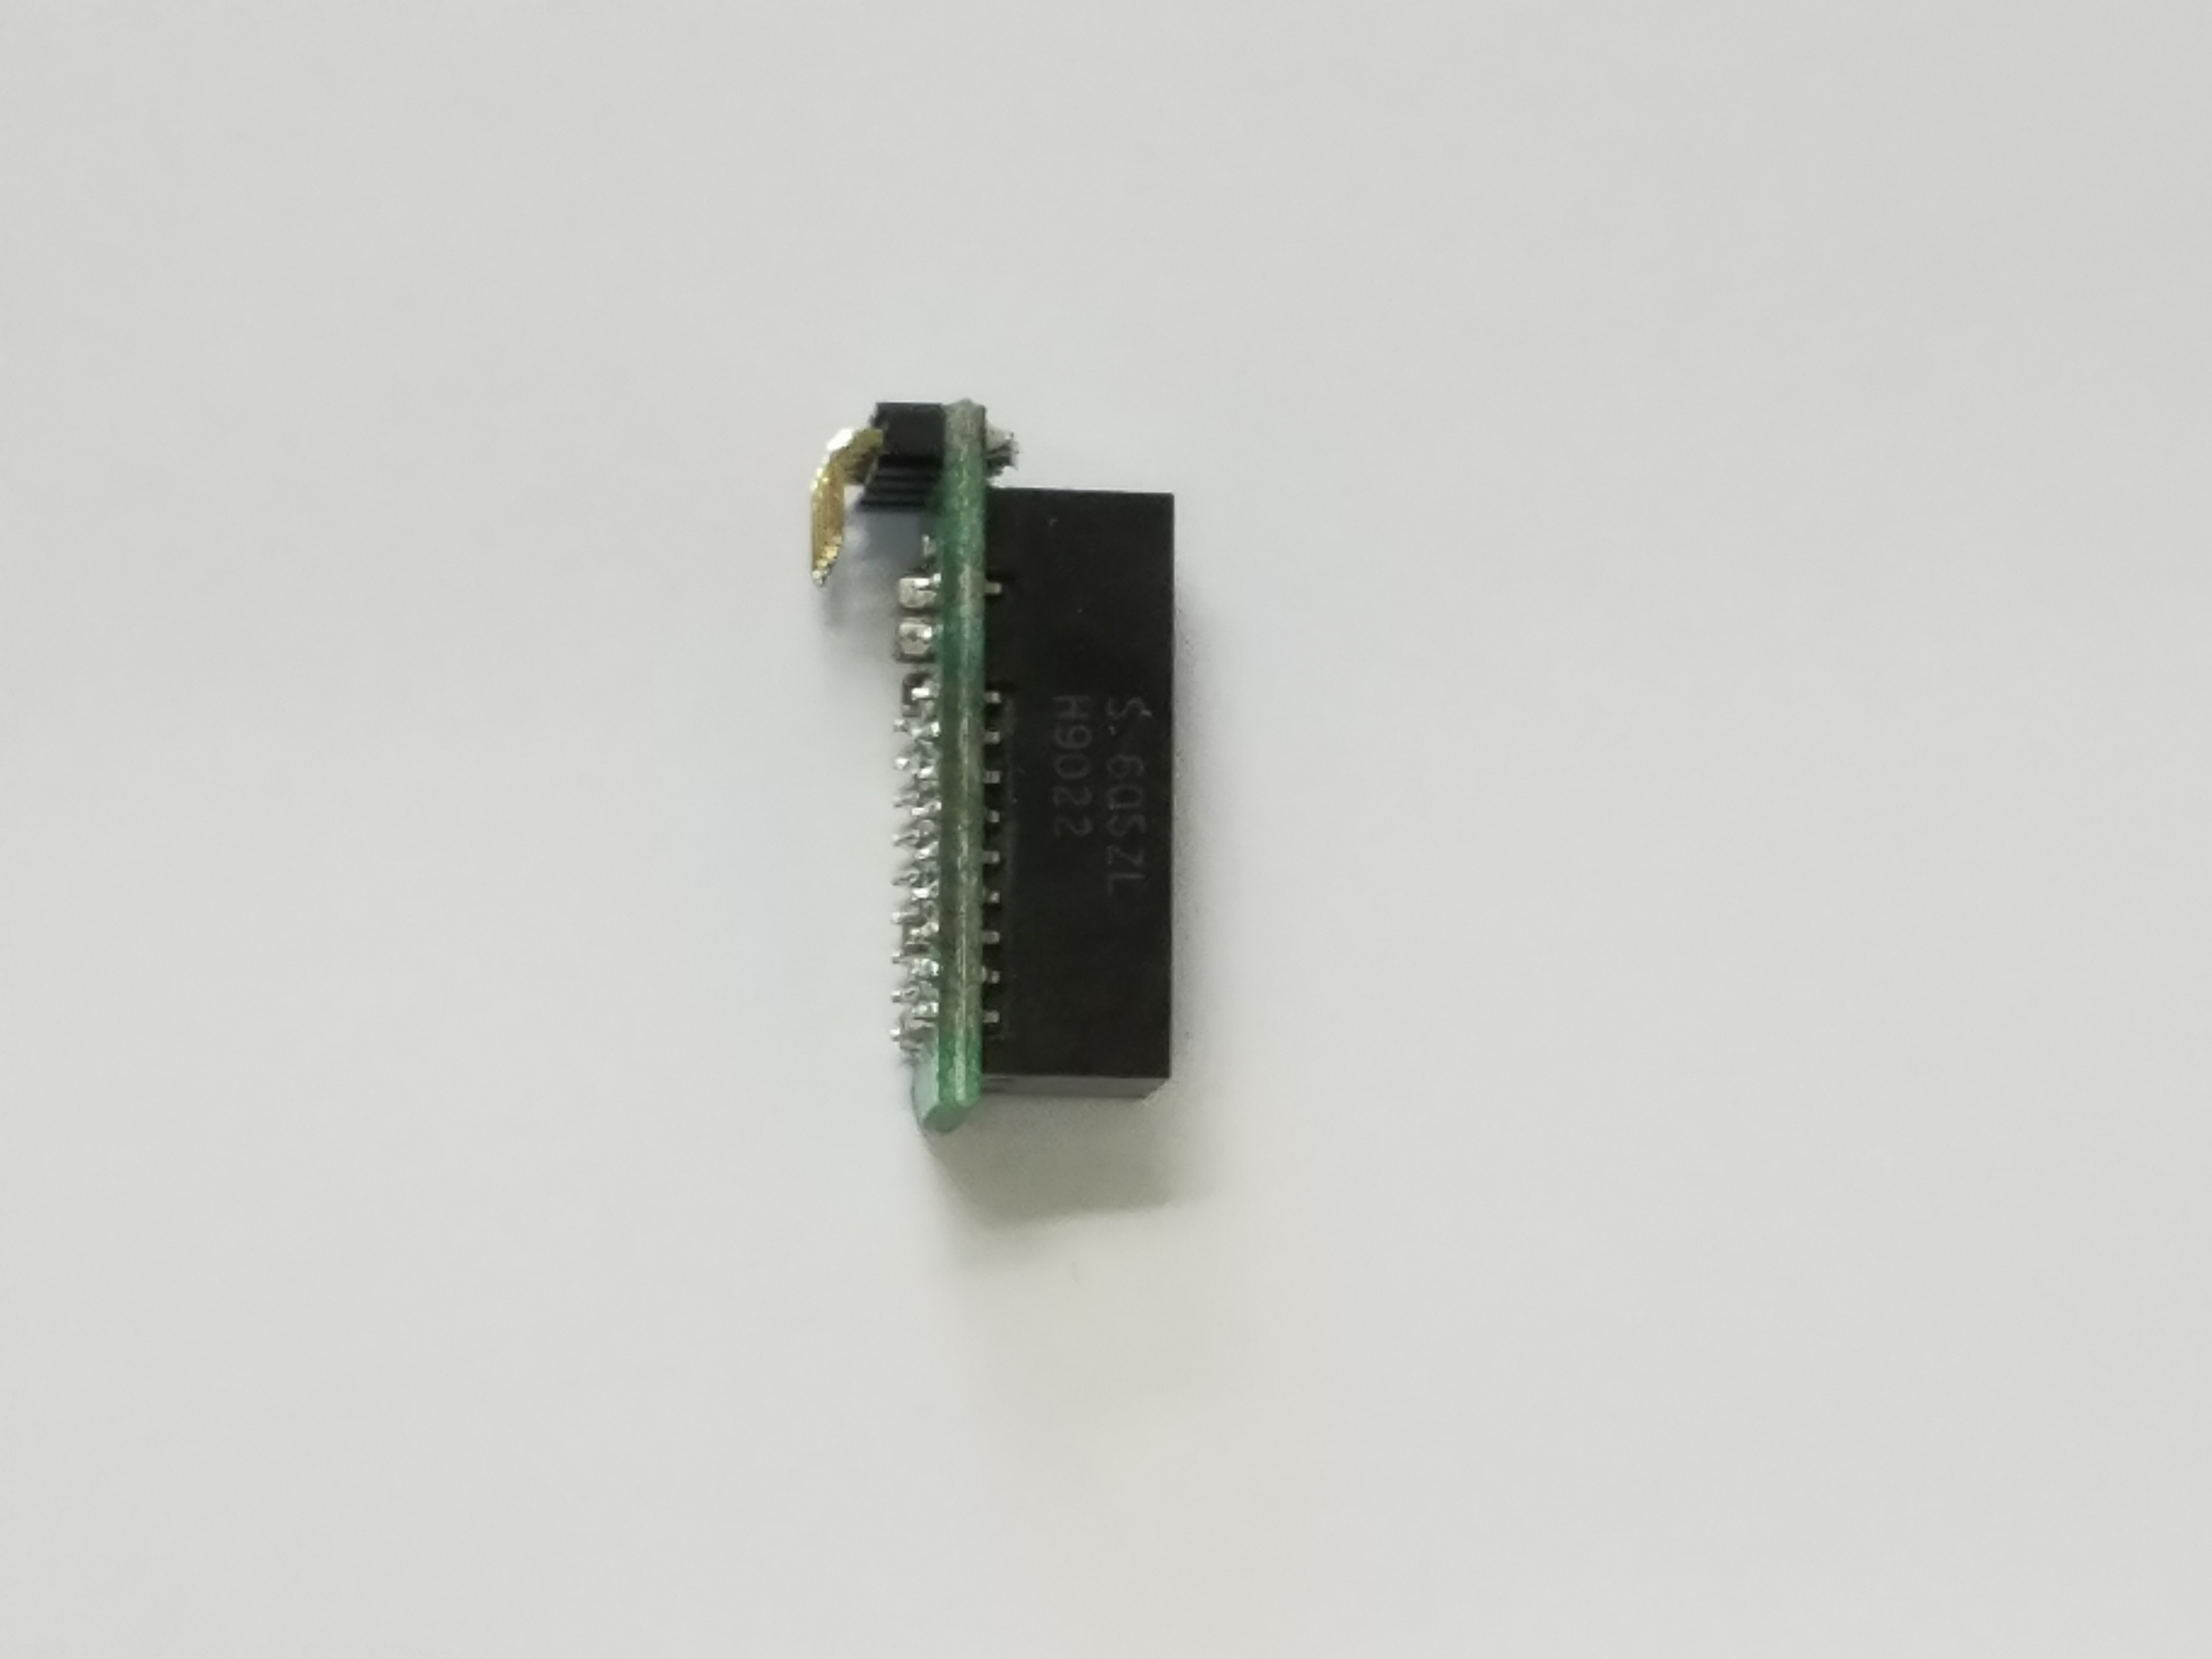
\includegraphics[width=0.445\columnwidth, keepaspectratio]{./figs/20181121_111525.jpg}}\\
\caption{Sharp infra-red distance sensor with headers properly attached.}
\label{fig:teesnySurfaceHeaderPerf}
\end{figure}
%End Male headers in PCB picture

\subsection{Populating the GRITSBot X Main PCB}
\label{sec:mainPCB}

 \subsubsection{Assembly Steps}
 
 \begin{enumerate}
 \item Gather the required materials (\cref{sec:mainPCBMaterials}).
 \item Solder the Teensy microcontroller, JST PH 2-Pin male header, and power switch (\cref{sec:solderTopComponents}).
 \item Solder the motor jumper cables (\cref{sec:solderMotorJumper}).
 \item Solder the IR sensors (\cref{sec:solderIRSensor}).
 \end{enumerate}
 
 \subsubsection{Required Materials}
 \label{sec:mainPCBMaterials}

All of the parts should now be ready to populate the main PCB of the GRITSBot X. To start we will add the Teensy 3.2, JST PH 2-Pin male header (power jumper for the Raspberry Pi), and main power switch. The materials you will need are pictured in \cref{fig:mainPCBFirstPass}.

%First Board Parts
\begin{figure}[h!]
\centering
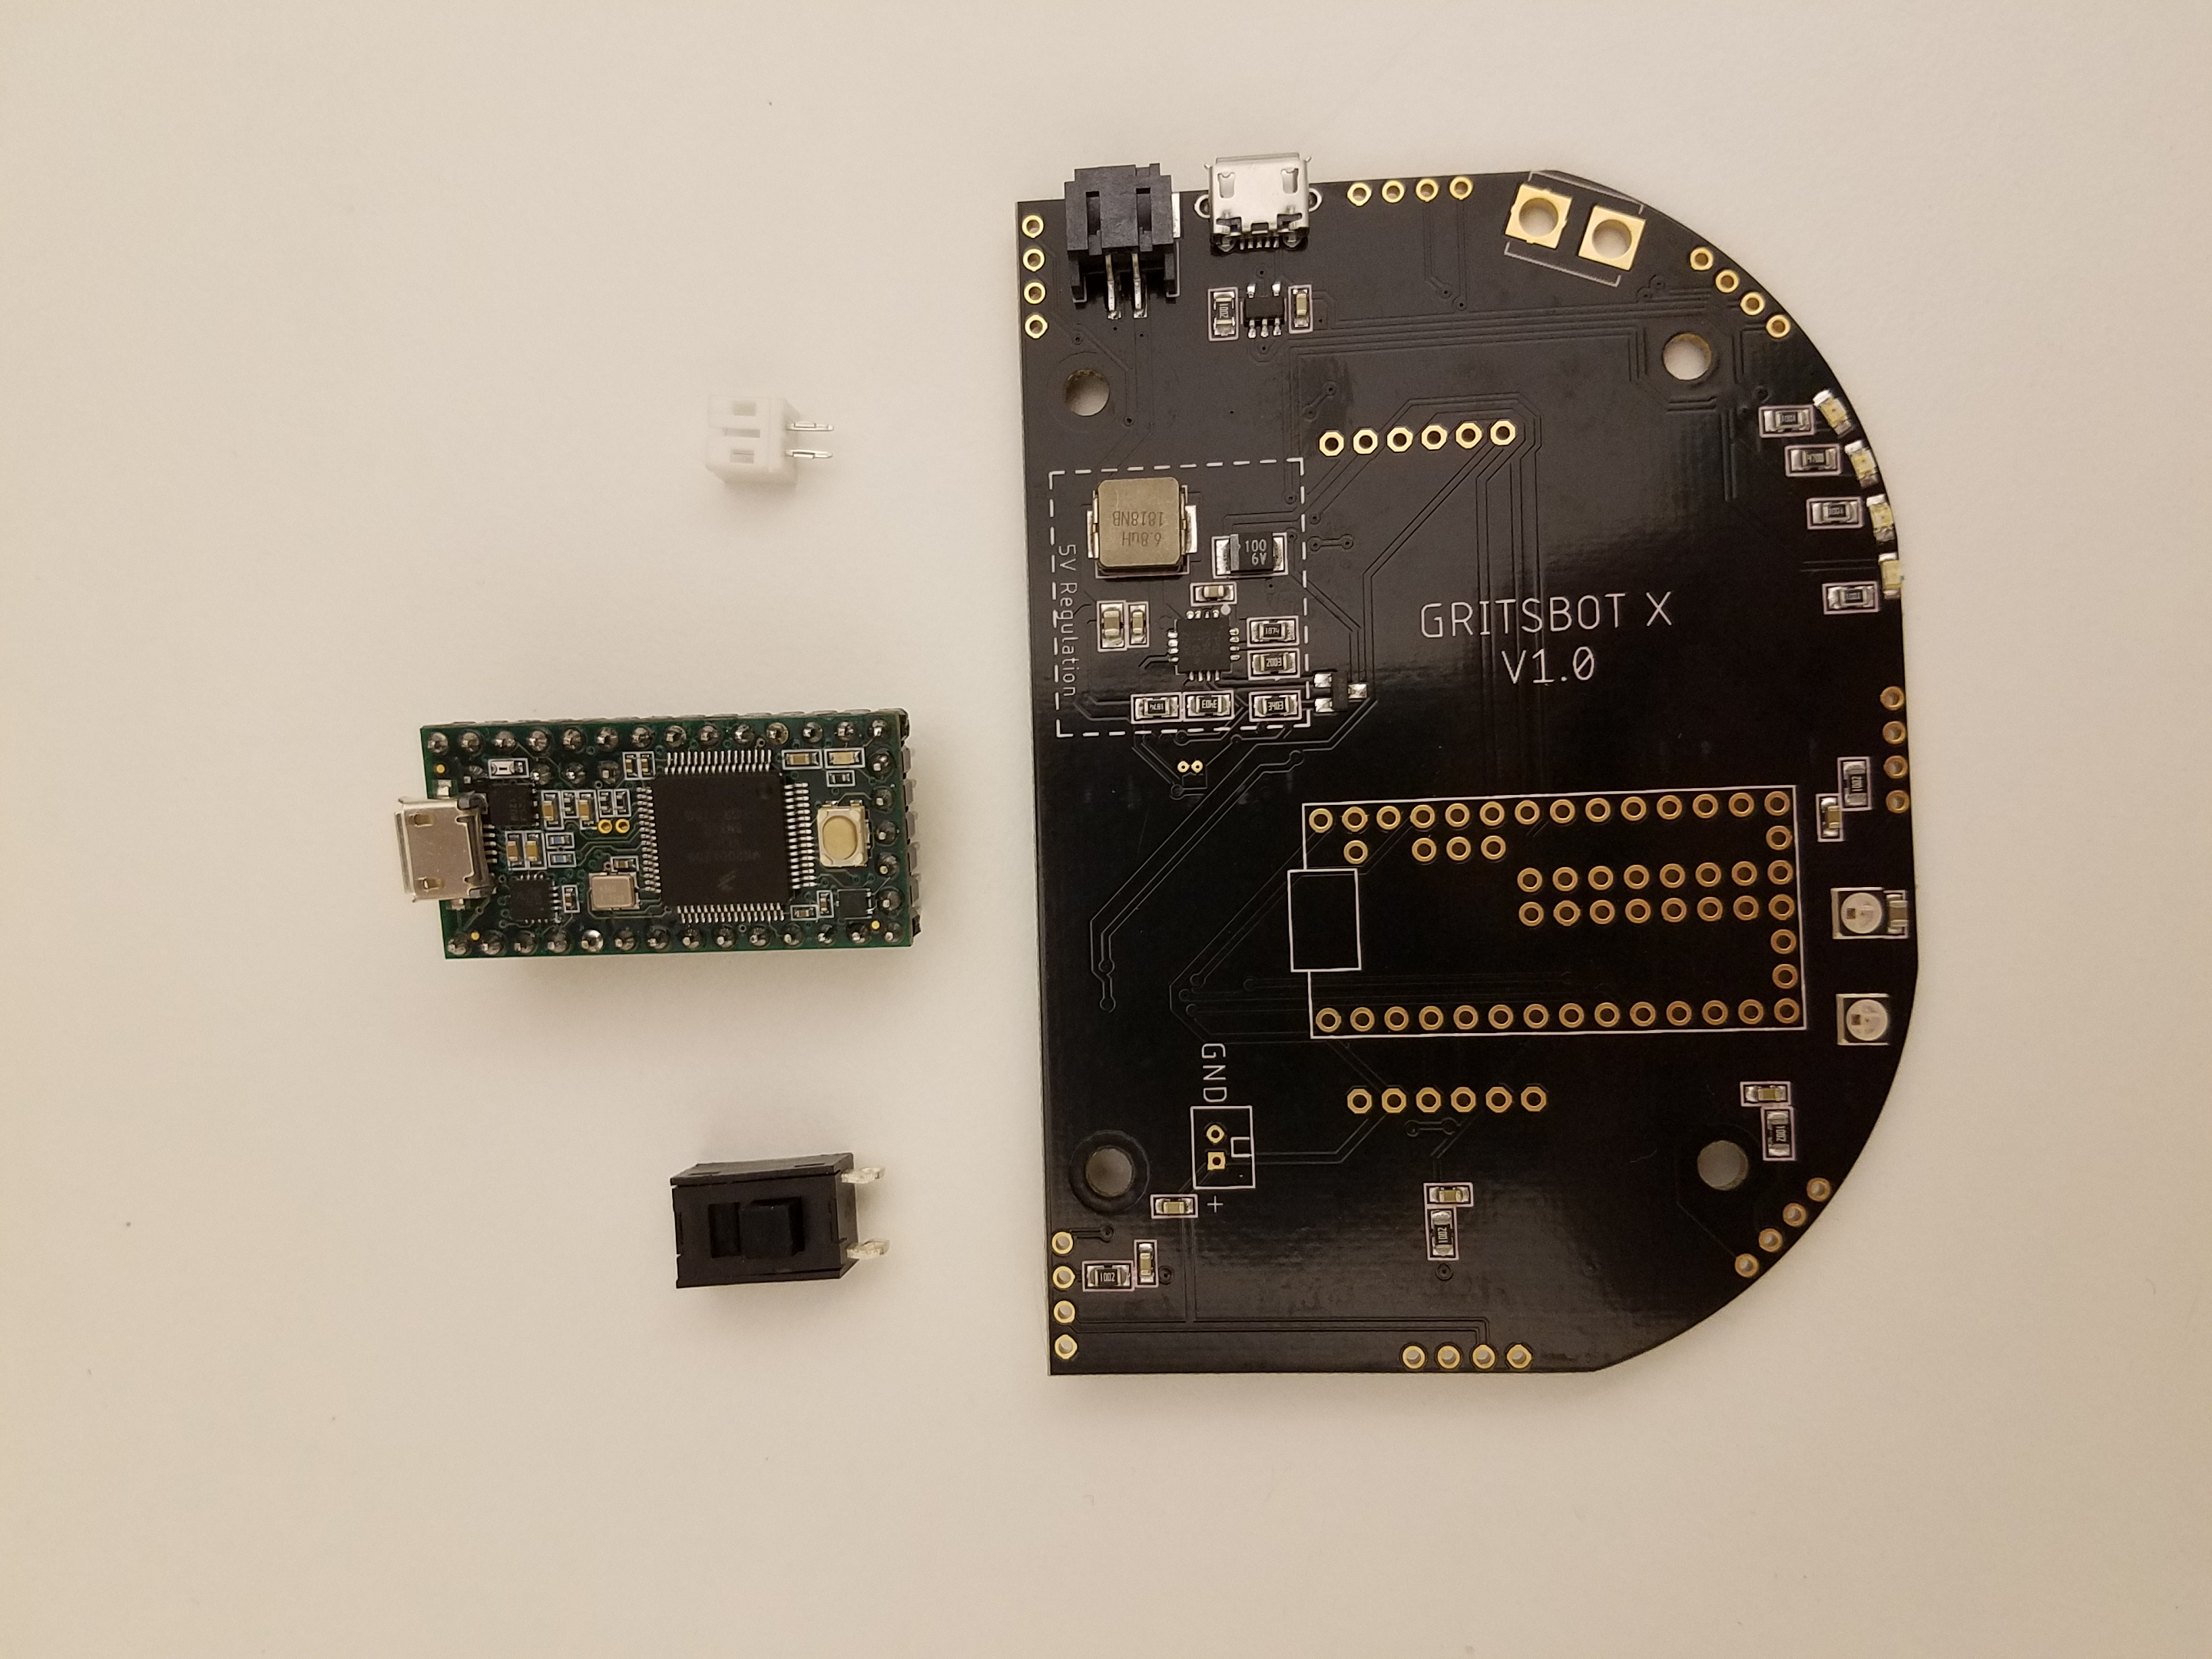
\includegraphics[width=0.65\columnwidth, keepaspectratio]{./figs/20180912_112215.jpg}
\caption{The materials for the first solder pass of the main PCB of the GRITSBot X.}
\label{fig:mainPCBFirstPass}
\end{figure}
%End First Board Parts

\subsubsection{Soldering the Top Through Hole Components}
\label{sec:solderTopComponents}

To start, first solder the Teensy into the main board (into the only spot where it fits). Make sure the Teensy is parallel with the main PCB of the GRITSBot X. To do this, lightly press the main chip of the Teensy into the main PCB. If this is not done, the connecting USB wire between the Teensy and Raspberry Pi (that will be added later) will not fit.

Next, place the ST PH 2-Pin male header (power jumper for the Raspberry Pi). It should be placed to the lower right of Teensy. The three openings on the side (meant for latching the female wire) should be facing the flat side of the board. You may have to press relatively hard as the tolerance of the drill for the main PCB may not be wide enough.

Finally, place the switch into the board (in the large holes to the left of the Teensy. Make sure the switch is facing the outside of the board and apply a large amount of solder. After finishing this, your board is ready to go minus the motors. Make sure all your solder connections are good and there are no cold joints or insufficient wetting. \cref{fig:mainPCBNoMotors} shows the top and bottom view of a completed board.

%First Populate Board
\begin{figure}[h!]
\centering
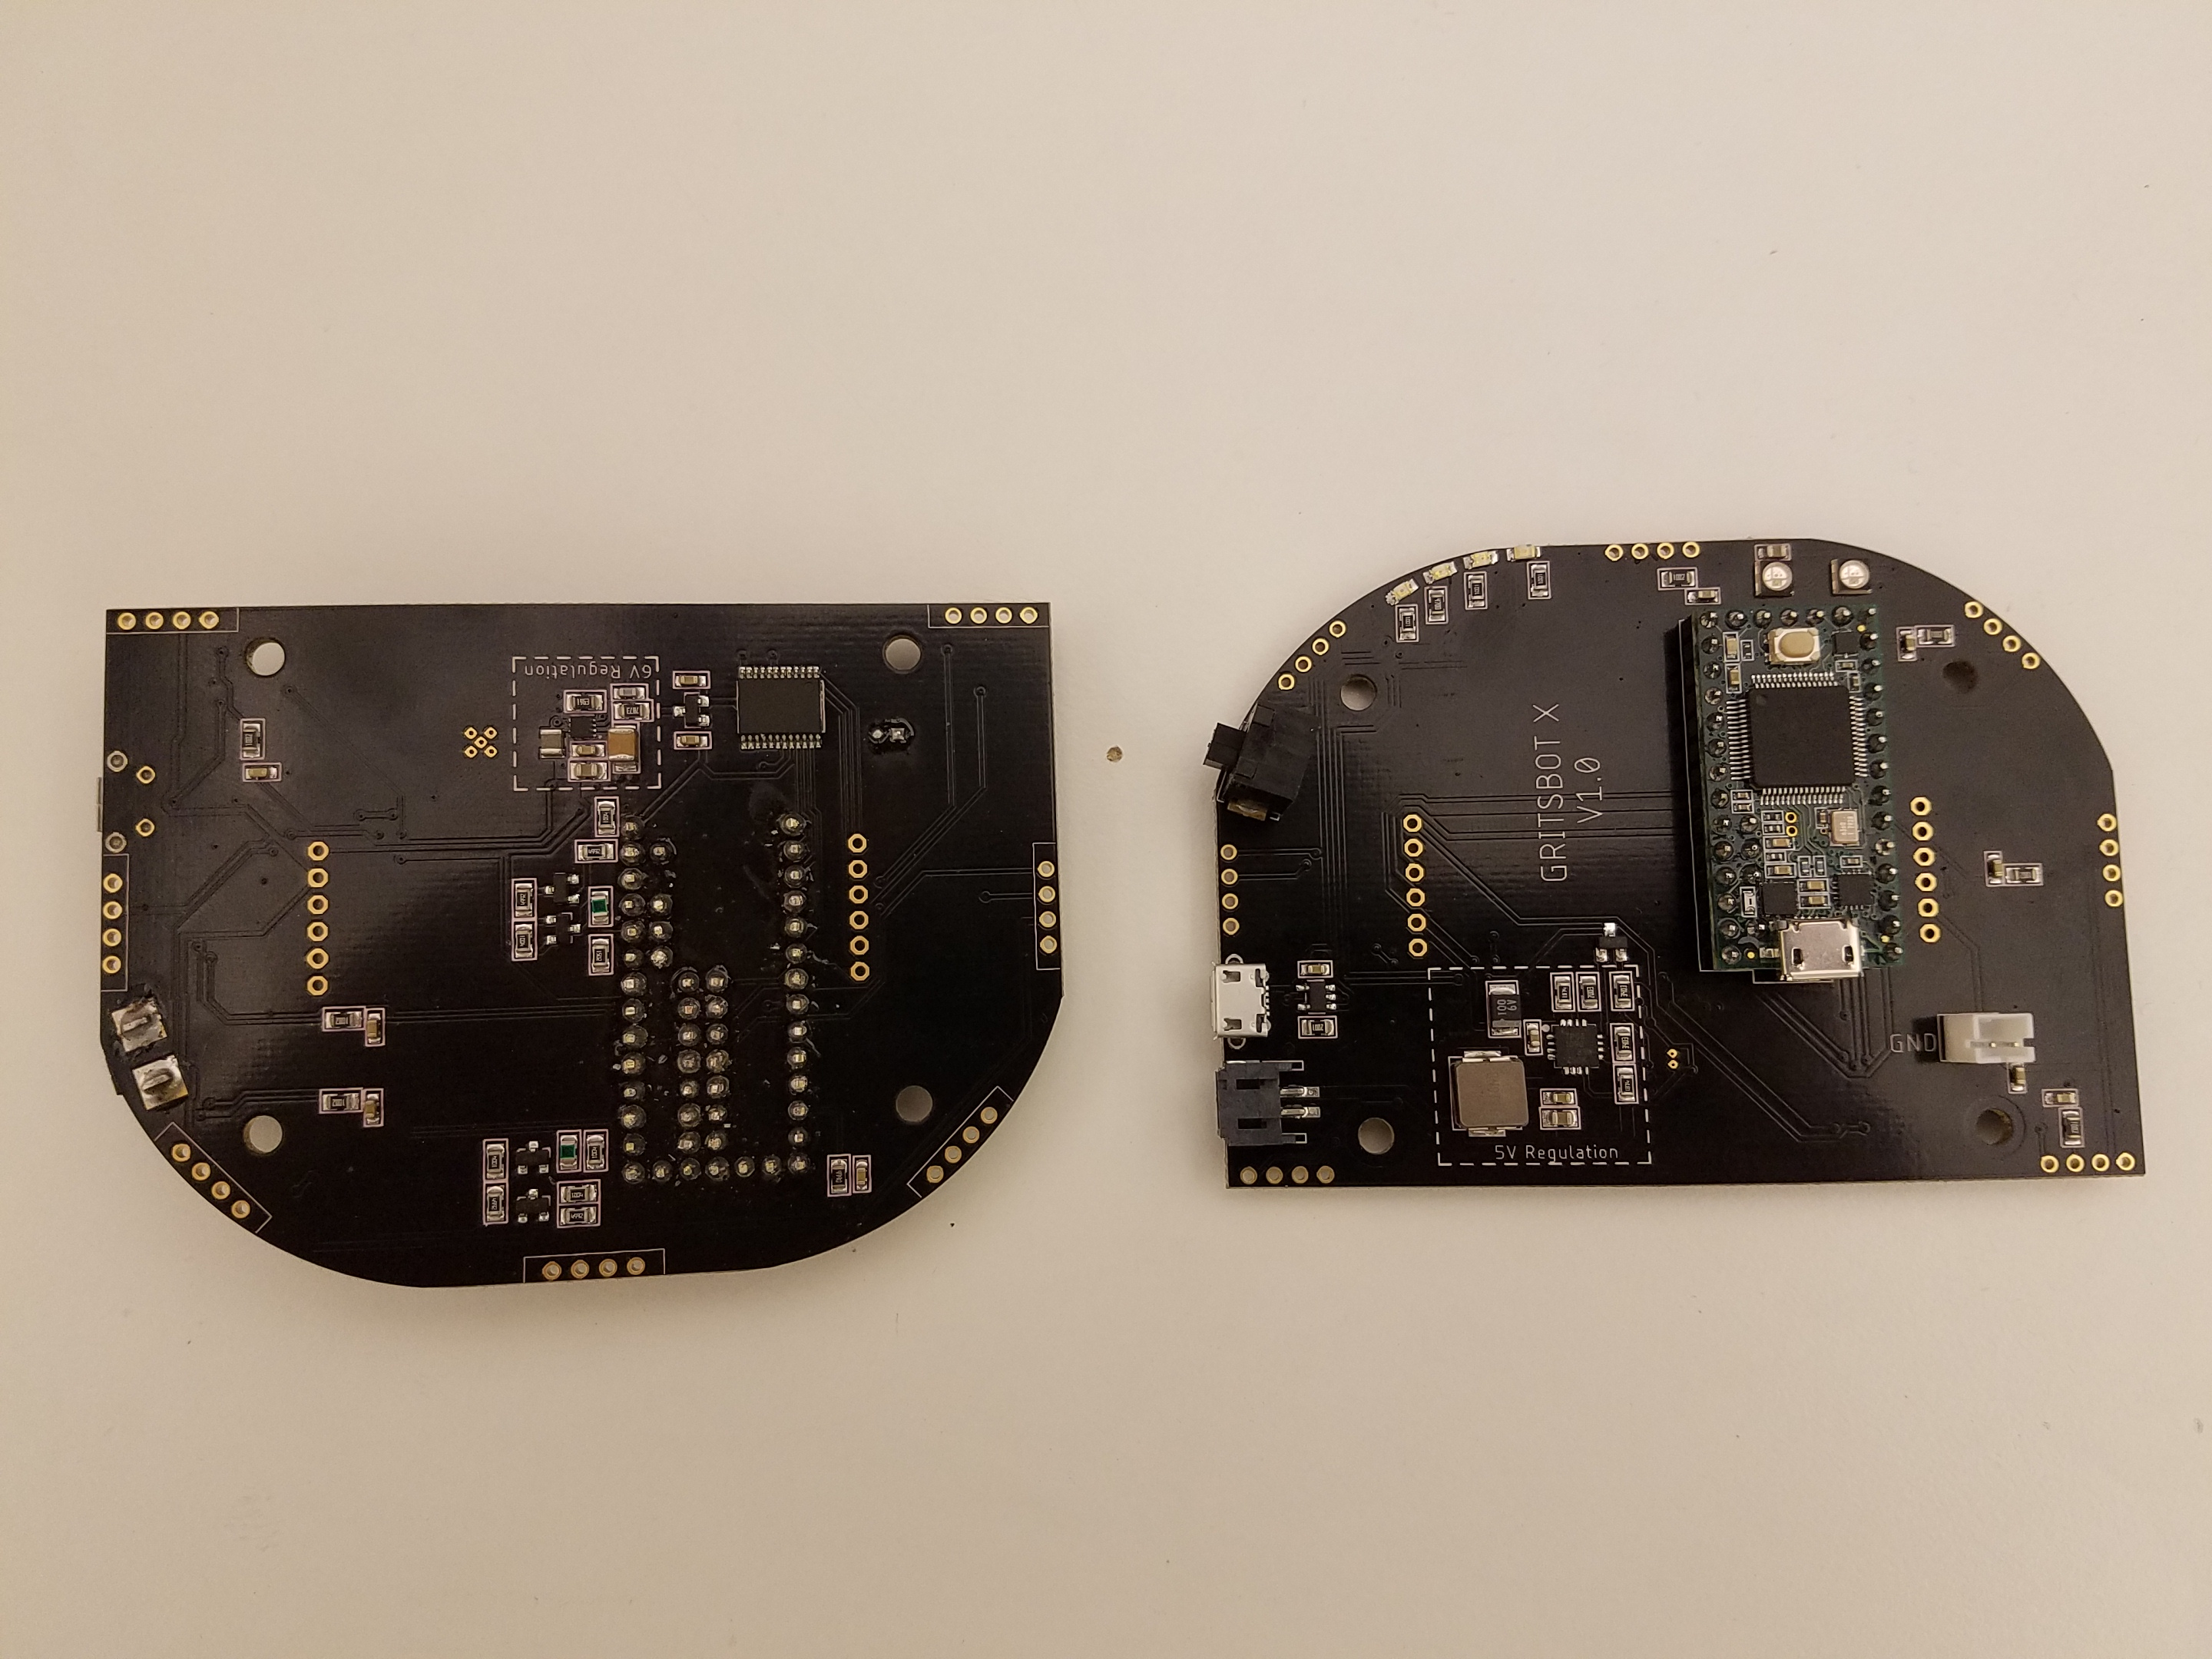
\includegraphics[width=0.65\columnwidth, keepaspectratio]{./figs/20180912_114341.jpg}
\caption{The GRITSBot X main PCB after mounting the Teesny microcontroller, JST PH 2-pin male header, and power switch.}
\label{fig:mainPCBNoMotors}
\end{figure}
%End First Populate Board

\subsubsection{Soldering the Motor and Encoder Leads}
\label{sec:solderMotorJumper}

The next parts to solder are the motor leads. This guide assumes you have purchased the micro metal gear motors with encoders attached from DFRobot. The row of six through holes correspond to the encoder attachments found on the DFRobot micro-metal gear motor. However, these pins are typically found in all quadrature shaft-encoders. From the top (curved edge) of the board to the bottom on both sides, the pins are: motor lead 1, ground, encoder output channel 1, encoder output channel 2, 5 volts, and motor lead 2. Make sure when soldering these they align with your motors correctly. This guide does not trim the motor leads shipped from DFRobot with the motors and instead coils the excess inside the robot. If you want you may cut the wire down to a smaller size but the stranded wire may be hard to keep from fraying out into a short when all six leads are attached. The wires connecting these motor leads are very small and can be tricky to attach without leaving too much excess exposed wire (which can lead to a short). A trick to make attaching these easier is to fill the through holes with solder and then heat the individual pad and insert the motor lead through the liquid solder. This allows you to slightly press and melt the insulation of the wire lead into the board which leaves no exposed metal. After attaching the motor leads, the bottom of the board should look like \cref{fig:finishedPCB}.

%Final Populate Board
\begin{figure}[h!]
\centering
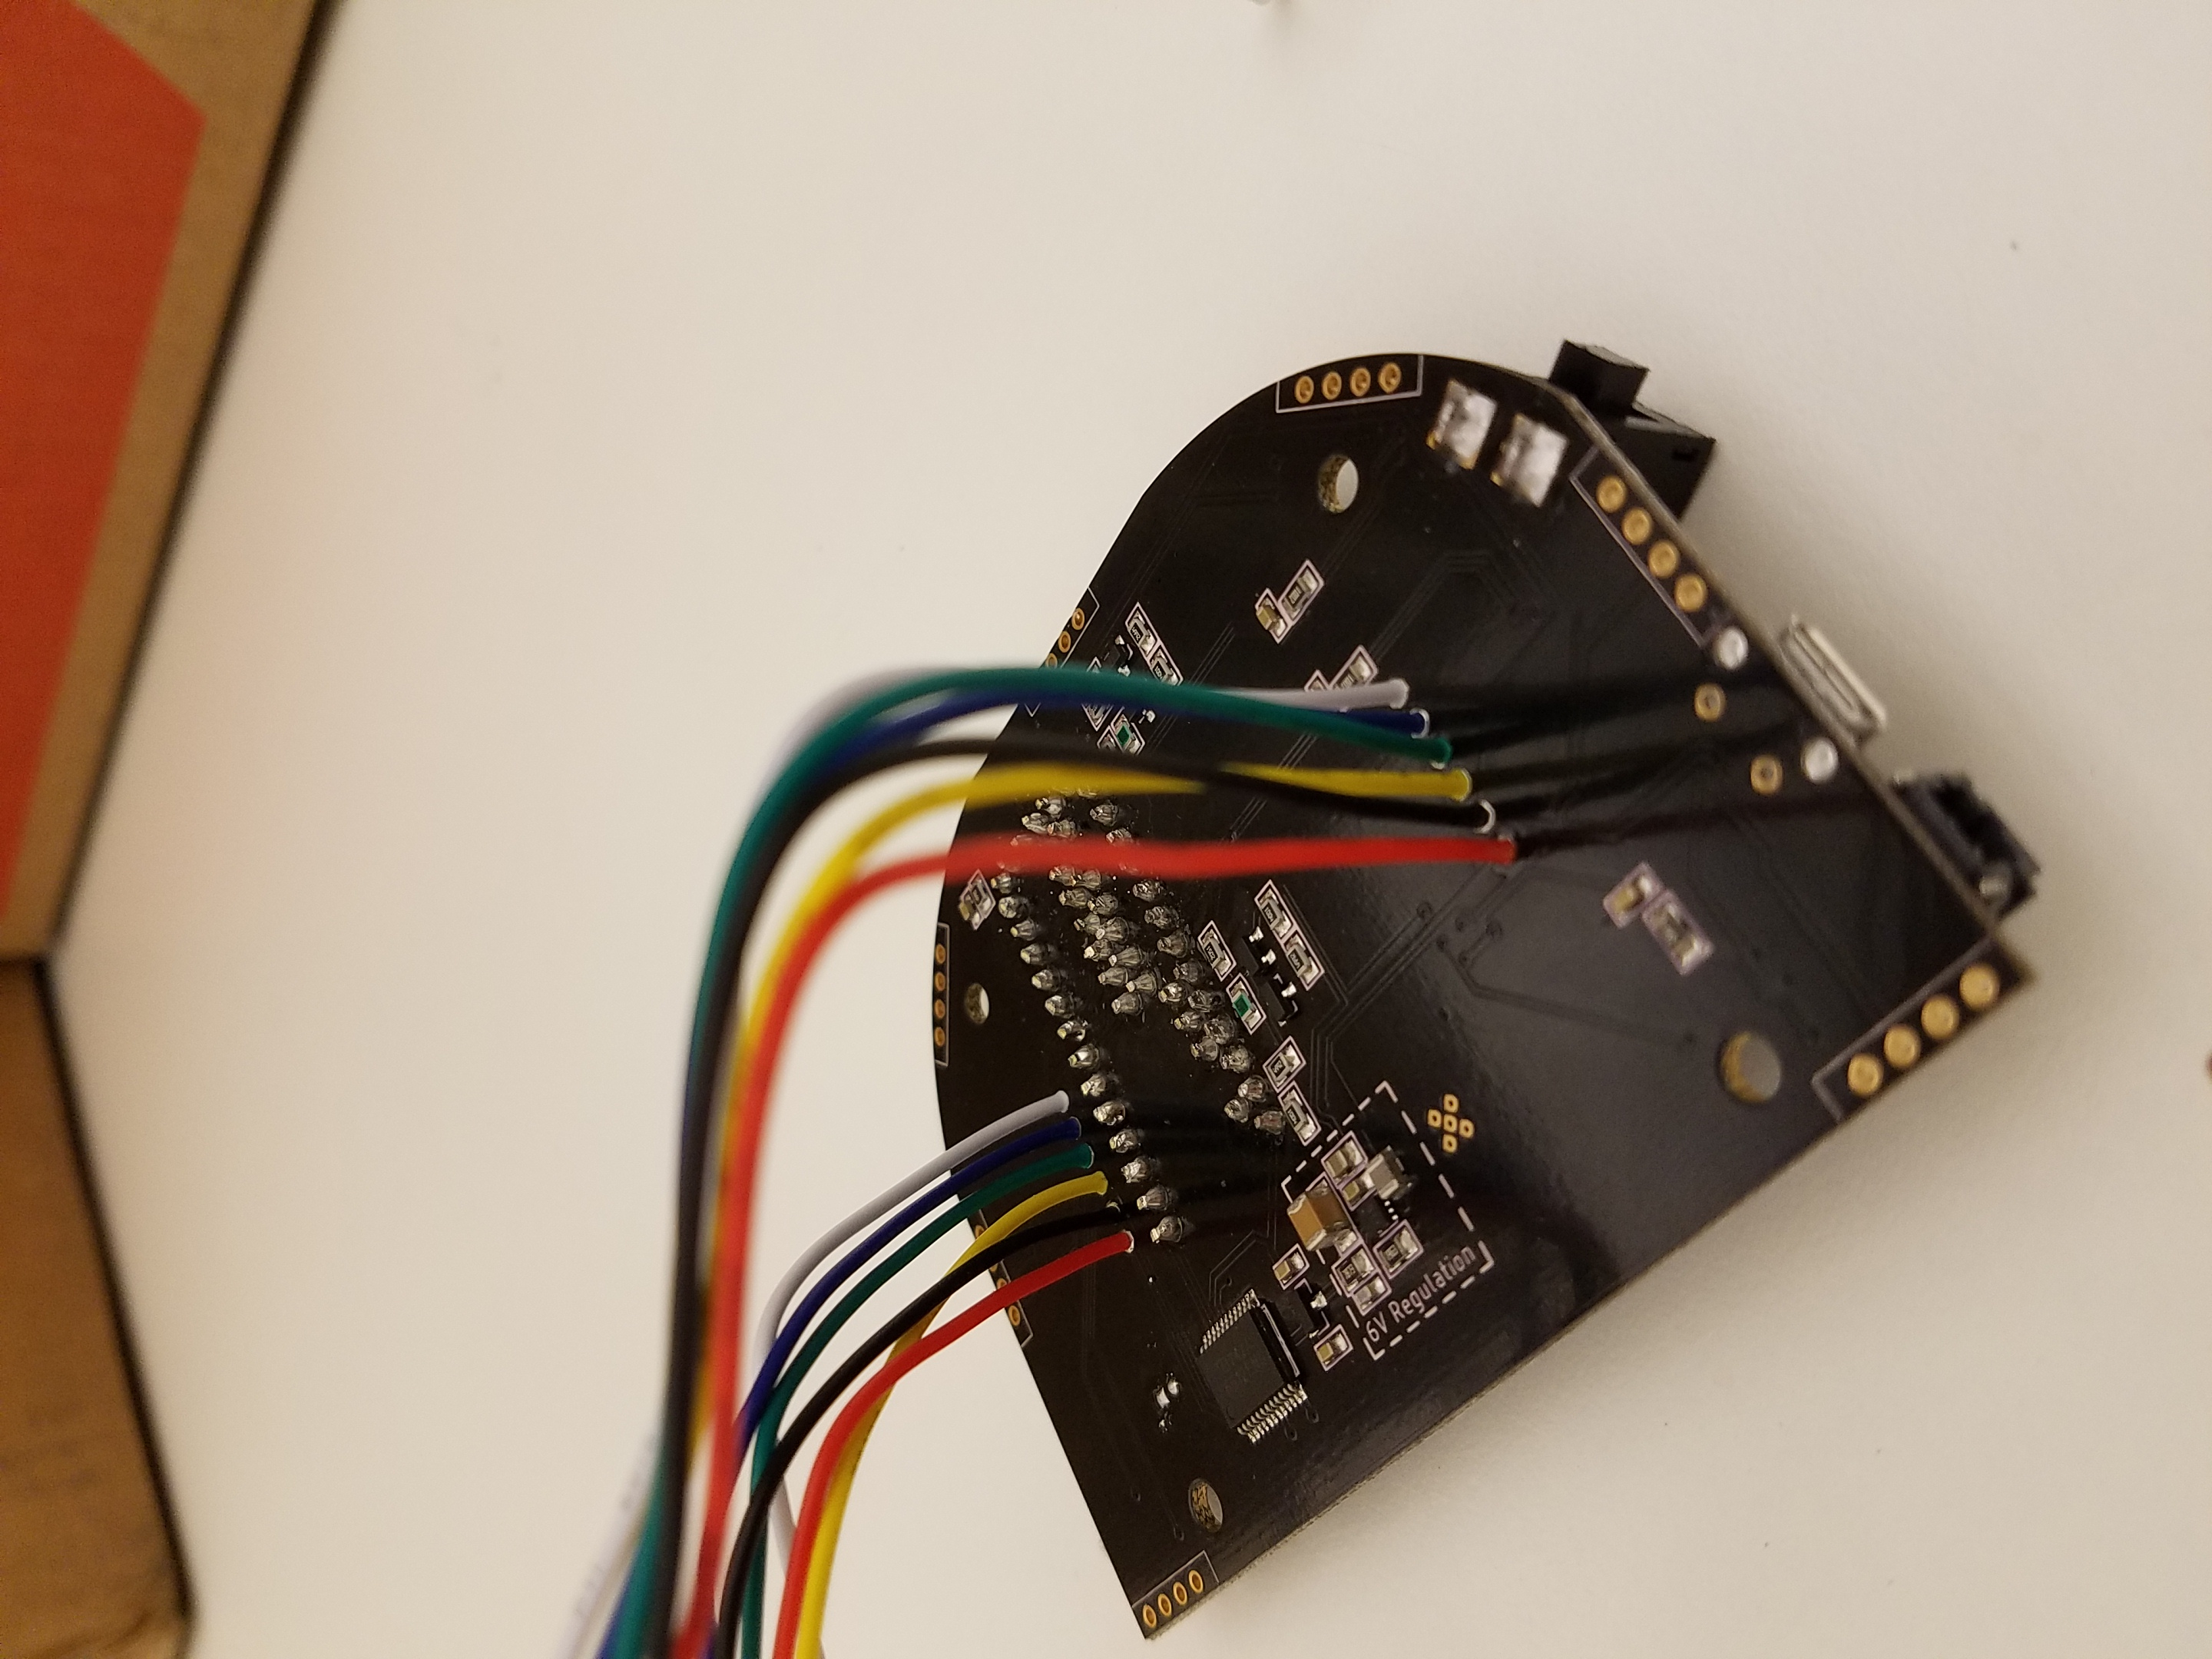
\includegraphics[width=0.65\columnwidth, keepaspectratio]{./figs/20180912_115521.jpg}
\caption{The GRITSBot X main PCB after mounting the motor leads.}
\label{fig:finishedPCB}
\end{figure}
%End Final Populate Board

\subsubsection{Soldering the IR Sensors}
\label{sec:solderIRSensor}

Finally we will attach the IR sensors around the perimeter of the main PCB. Hang the sensors on the GRITSBot X main PCB such that the sensor hangs below the board (the side with the motor cables). To solder this, it is easier to solder the the pins from the angled side first and let the capillary action pull the solder through. You will also want to solder one pin and make sure the sensor is perpendicular to the main PCB. After the sensor is perpendicular, solder the other four pins and continue to populate the other six sensor slots.

\subsection{Wire Leads to the Raspberry Pi Zero W}
\label{sec:raspberryPiLeads}
To compliment the Teensy microcontroller on the main PCB of the GRITSBot X, the robot also uses a Raspberry Pi Zero W. This board is powered through the GPIO pins of the board. To achieve this solder the JST PH 2-Pin Cable - Female Connector to pin numbers 4 and 6 where 4 is the positive lead and 6 is the ground lead. Make sure this connection is donw with the correct polarity, if it does not you will destroy the Raspberry Pi Zero W.